\documentclass[english]{article}
%DIF LATEXDIFF DIFFERENCE FILE
%DIF DEL old.tex    Wed Aug 11 10:03:33 2021
%DIF ADD main.tex   Wed Aug 11 10:21:36 2021
\usepackage{graphicx}
\usepackage{amsmath}
\usepackage{hyperref}
\usepackage{setspace}
\usepackage{apacite}
\usepackage{hyperref}
\usepackage[sort]{natbib}
\usepackage[font=small,labelfont=bf]{caption} %DIF > 
\usepackage[sort&compress, numbers, super]{natbib} %DIF > 
%DIF -------
\usepackage{pxfonts}
\usepackage[utf8]{inputenc}
\usepackage[left=1in,right=1in,top=1in,bottom=1in]{geometry}
\usepackage[left]{lineno}
\usepackage{soul}
%DIF 14a14
\usepackage[nofiglist, fighead]{endfloat} %DIF > 
%DIF -------
\linenumbers

\newcommand{\kernelshape}{S1}
\newcommand{\kernelwidth}{S2}
\newcommand{\timeheatmap}{S3}
\newcommand{\features}{S4}
\newcommand{\intact}{S5}
\newcommand{\para}{S6}
\newcommand{\word}{S7}
\newcommand{\rest}{S8}
\newcommand{\pca}{S9}

\title{High-level cognition during story listening is reflected in
  high-order dynamic correlations in neural activity patterns}

\author{Lucy L. W. Owen$^1$, Thomas H. Chang$^{1,2}$, and\
  Jeremy R. Manning\textsuperscript{$1, \dagger$}\\
  [0.1in]$^1$Department of Psychological and Brain
  Sciences,\\Dartmouth
  College, Hanover, NH\\
  $^2$Amazon.com, Seattle, WA\\
  \textsuperscript{$\dagger$}Address correspondence to
  jeremy.r.manning@dartmouth.edu}
%DIF PREAMBLE EXTENSION ADDED BY LATEXDIFF
%DIF UNDERLINE PREAMBLE %DIF PREAMBLE
\RequirePackage[normalem]{ulem} %DIF PREAMBLE
\RequirePackage{color}\definecolor{RED}{rgb}{1,0,0}\definecolor{BLUE}{rgb}{0,0,1} %DIF PREAMBLE
\providecommand{\DIFaddtex}[1]{{\protect\color{blue}\uwave{#1}}} %DIF PREAMBLE
\providecommand{\DIFdeltex}[1]{{\protect\color{red}\sout{#1}}}                      %DIF PREAMBLE
%DIF SAFE PREAMBLE %DIF PREAMBLE
\providecommand{\DIFaddbegin}{} %DIF PREAMBLE
\providecommand{\DIFaddend}{} %DIF PREAMBLE
\providecommand{\DIFdelbegin}{} %DIF PREAMBLE
\providecommand{\DIFdelend}{} %DIF PREAMBLE
\providecommand{\DIFmodbegin}{} %DIF PREAMBLE
\providecommand{\DIFmodend}{} %DIF PREAMBLE
%DIF FLOATSAFE PREAMBLE %DIF PREAMBLE
\providecommand{\DIFaddFL}[1]{\DIFadd{#1}} %DIF PREAMBLE
\providecommand{\DIFdelFL}[1]{\DIFdel{#1}} %DIF PREAMBLE
\providecommand{\DIFaddbeginFL}{} %DIF PREAMBLE
\providecommand{\DIFaddendFL}{} %DIF PREAMBLE
\providecommand{\DIFdelbeginFL}{} %DIF PREAMBLE
\providecommand{\DIFdelendFL}{} %DIF PREAMBLE
%DIF HYPERREF PREAMBLE %DIF PREAMBLE
\providecommand{\DIFadd}[1]{\texorpdfstring{\DIFaddtex{#1}}{#1}} %DIF PREAMBLE
\providecommand{\DIFdel}[1]{\texorpdfstring{\DIFdeltex{#1}}{}} %DIF PREAMBLE
\newcommand{\DIFscaledelfig}{0.5}
%DIF HIGHLIGHTGRAPHICS PREAMBLE %DIF PREAMBLE
\RequirePackage{settobox} %DIF PREAMBLE
\RequirePackage{letltxmacro} %DIF PREAMBLE
\newsavebox{\DIFdelgraphicsbox} %DIF PREAMBLE
\newlength{\DIFdelgraphicswidth} %DIF PREAMBLE
\newlength{\DIFdelgraphicsheight} %DIF PREAMBLE
% store original definition of \includegraphics %DIF PREAMBLE
\LetLtxMacro{\DIFOincludegraphics}{\includegraphics} %DIF PREAMBLE
\newcommand{\DIFaddincludegraphics}[2][]{{\color{blue}\fbox{\DIFOincludegraphics[#1]{#2}}}} %DIF PREAMBLE
\newcommand{\DIFdelincludegraphics}[2][]{% %DIF PREAMBLE
\sbox{\DIFdelgraphicsbox}{\DIFOincludegraphics[#1]{#2}}% %DIF PREAMBLE
\settoboxwidth{\DIFdelgraphicswidth}{\DIFdelgraphicsbox} %DIF PREAMBLE
\settoboxtotalheight{\DIFdelgraphicsheight}{\DIFdelgraphicsbox} %DIF PREAMBLE
\scalebox{\DIFscaledelfig}{% %DIF PREAMBLE
\parbox[b]{\DIFdelgraphicswidth}{\usebox{\DIFdelgraphicsbox}\\[-\baselineskip] \rule{\DIFdelgraphicswidth}{0em}}\llap{\resizebox{\DIFdelgraphicswidth}{\DIFdelgraphicsheight}{% %DIF PREAMBLE
\setlength{\unitlength}{\DIFdelgraphicswidth}% %DIF PREAMBLE
\begin{picture}(1,1)% %DIF PREAMBLE
\thicklines\linethickness{2pt} %DIF PREAMBLE
{\color[rgb]{1,0,0}\put(0,0){\framebox(1,1){}}}% %DIF PREAMBLE
{\color[rgb]{1,0,0}\put(0,0){\line( 1,1){1}}}% %DIF PREAMBLE
{\color[rgb]{1,0,0}\put(0,1){\line(1,-1){1}}}% %DIF PREAMBLE
\end{picture}% %DIF PREAMBLE
}\hspace*{3pt}}} %DIF PREAMBLE
} %DIF PREAMBLE
\LetLtxMacro{\DIFOaddbegin}{\DIFaddbegin} %DIF PREAMBLE
\LetLtxMacro{\DIFOaddend}{\DIFaddend} %DIF PREAMBLE
\LetLtxMacro{\DIFOdelbegin}{\DIFdelbegin} %DIF PREAMBLE
\LetLtxMacro{\DIFOdelend}{\DIFdelend} %DIF PREAMBLE
\DeclareRobustCommand{\DIFaddbegin}{\DIFOaddbegin \let\includegraphics\DIFaddincludegraphics} %DIF PREAMBLE
\DeclareRobustCommand{\DIFaddend}{\DIFOaddend \let\includegraphics\DIFOincludegraphics} %DIF PREAMBLE
\DeclareRobustCommand{\DIFdelbegin}{\DIFOdelbegin \let\includegraphics\DIFdelincludegraphics} %DIF PREAMBLE
\DeclareRobustCommand{\DIFdelend}{\DIFOaddend \let\includegraphics\DIFOincludegraphics} %DIF PREAMBLE
\LetLtxMacro{\DIFOaddbeginFL}{\DIFaddbeginFL} %DIF PREAMBLE
\LetLtxMacro{\DIFOaddendFL}{\DIFaddendFL} %DIF PREAMBLE
\LetLtxMacro{\DIFOdelbeginFL}{\DIFdelbeginFL} %DIF PREAMBLE
\LetLtxMacro{\DIFOdelendFL}{\DIFdelendFL} %DIF PREAMBLE
\DeclareRobustCommand{\DIFaddbeginFL}{\DIFOaddbeginFL \let\includegraphics\DIFaddincludegraphics} %DIF PREAMBLE
\DeclareRobustCommand{\DIFaddendFL}{\DIFOaddendFL \let\includegraphics\DIFOincludegraphics} %DIF PREAMBLE
\DeclareRobustCommand{\DIFdelbeginFL}{\DIFOdelbeginFL \let\includegraphics\DIFdelincludegraphics} %DIF PREAMBLE
\DeclareRobustCommand{\DIFdelendFL}{\DIFOaddendFL \let\includegraphics\DIFOincludegraphics} %DIF PREAMBLE
%DIF LISTINGS PREAMBLE %DIF PREAMBLE
\RequirePackage{listings} %DIF PREAMBLE
\RequirePackage{color} %DIF PREAMBLE
\lstdefinelanguage{DIFcode}{ %DIF PREAMBLE
%DIF DIFCODE_UNDERLINE %DIF PREAMBLE
  moredelim=[il][\color{red}\sout]{\%DIF\ <\ }, %DIF PREAMBLE
  moredelim=[il][\color{blue}\uwave]{\%DIF\ >\ } %DIF PREAMBLE
} %DIF PREAMBLE
\lstdefinestyle{DIFverbatimstyle}{ %DIF PREAMBLE
	language=DIFcode, %DIF PREAMBLE
	basicstyle=\ttfamily, %DIF PREAMBLE
	columns=fullflexible, %DIF PREAMBLE
	keepspaces=true %DIF PREAMBLE
} %DIF PREAMBLE
\lstnewenvironment{DIFverbatim}{\lstset{style=DIFverbatimstyle}}{} %DIF PREAMBLE
\lstnewenvironment{DIFverbatim*}{\lstset{style=DIFverbatimstyle,showspaces=true}}{} %DIF PREAMBLE
%DIF END PREAMBLE EXTENSION ADDED BY LATEXDIFF

\begin{document}
\maketitle


\begin{abstract}
  Our thoughts arise from coordinated patterns of interactions between
  brain structures that change with our ongoing experiences.
  High-order dynamic correlations in neural activity patterns reflect
  different subgraphs of the brain's functional connectome that display
  homologous lower-level dynamic correlations.  \DIFdelbegin \DIFdel{We tested }\DIFdelend \DIFaddbegin \DIFadd{Here we test }\DIFaddend the
  hypothesis that high-level cognition is reflected in high-order
  dynamic correlations in brain activity patterns.  We \DIFdelbegin \DIFdel{developed }\DIFdelend \DIFaddbegin \DIFadd{develop }\DIFaddend an
  approach to estimating high-order dynamic correlations in timeseries
  data, and we \DIFdelbegin \DIFdel{applied }\DIFdelend \DIFaddbegin \DIFadd{apply }\DIFaddend the approach to neuroimaging data collected as
  human participants either \DIFdelbegin \DIFdel{listened }\DIFdelend \DIFaddbegin \DIFadd{listen }\DIFaddend to a ten-minute story or \DIFdelbegin \DIFdel{listened
  }\DIFdelend \DIFaddbegin \DIFadd{listen
  }\DIFaddend to a temporally scrambled version of the story.  We \DIFdelbegin \DIFdel{trained
  }\DIFdelend \DIFaddbegin \DIFadd{train
  }\DIFaddend across-participant pattern classifiers to decode (in held-out data)
  when in the session each neural activity snapshot was collected.  We
  \DIFdelbegin \DIFdel{found }\DIFdelend \DIFaddbegin \DIFadd{find }\DIFaddend that classifiers trained to decode from high-order dynamic
  correlations \DIFdelbegin \DIFdel{yielded }\DIFdelend \DIFaddbegin \DIFadd{yield }\DIFaddend the best performance on data collected as
  participants listened to the (unscrambled) story.  By contrast,
  classifiers trained to decode data from scrambled versions of the
  story yielded the best performance when they were trained using
  first-order dynamic correlations or non-correlational activity
  patterns.  We suggest that as our thoughts become more complex, they
  are reflected in higher-order patterns of dynamic network
  interactions throughout the brain.
\end{abstract}

\doublespacing

\section*{Introduction}
A central goal in cognitive neuroscience is to elucidate the
\DIFdelbegin \textit{\DIFdel{neural code}}%DIFAUXCMD
\DIFdel{: }\DIFdelend \DIFaddbegin \DIFadd{neural code: i.e., }\DIFaddend the mapping between (a) mental states or
cognitive representations and (b) neural activity patterns. One means
of testing models of the neural code is to ask how accurately that
model is able to ``translate'' neural activity patterns into known (or
hypothesized) mental states or cognitive
representations~\DIFdelbegin \DIFdel{\mbox{%DIFAUXCMD
\citep[e.g.,][]{HaxbEtal01, NormEtal06b, TongPrat12,
  MitcEtal08a, KamiTong05, NishEtal11, PereEtal18, HuthEtal12,
  HuthEtal16}}\hspace{0pt}%DIFAUXCMD
}\DIFdelend \DIFaddbegin \DIFadd{\mbox{%DIFAUXCMD
\cite{HaxbEtal01, NormEtal06b, TongPrat12,
  MitcEtal08a, KamiTong05, NishEtal11, PereEtal18, HuthEtal12,
  HuthEtal16}}\hspace{0pt}%DIFAUXCMD
}\DIFaddend .  Training decoding models on different types of neural
features (Fig.~\ref{fig:patterns}a) can also help to elucidate which
specific aspects of neural activity patterns are informative about
cognition and, by extension, which types of neural activity patterns
might compose the neural code.  For example, prior work has used
region of interest analyses to estimate the anatomical locations of
specific neural representations~\DIFdelbegin \DIFdel{\mbox{%DIFAUXCMD
\citep[e.g.,][]{EtzeEtal09}}\hspace{0pt}%DIFAUXCMD
}\DIFdelend \DIFaddbegin \DIFadd{\mbox{%DIFAUXCMD
\cite{EtzeEtal09}}\hspace{0pt}%DIFAUXCMD
}\DIFaddend , or to
compare the relative contributions to the neural code of multivariate
activity patterns versus dynamic correlations between neural activity
patterns~\DIFdelbegin \DIFdel{\mbox{%DIFAUXCMD
\citep[e.g.,][]{MannEtal18, FongEtal19}}\hspace{0pt}%DIFAUXCMD
}\DIFdelend \DIFaddbegin \DIFadd{\mbox{%DIFAUXCMD
\cite{MannEtal18, FongEtal19}}\hspace{0pt}%DIFAUXCMD
}\DIFaddend .  An emerging theme
in this literature is that cognition is mediated by dynamic
interactions between brain structures~\DIFdelbegin \DIFdel{\mbox{%DIFAUXCMD
\citep{Gros88, Fris00, SporHone06, BassEtal06,
  Turk13, DemeEtal19, SoloEtal19, LuriEtal18, PretEtal17, ZouEtal19,
  MackEtal17, BresKels01, McIn00}}\hspace{0pt}%DIFAUXCMD
}\DIFdelend \DIFaddbegin \DIFadd{\mbox{%DIFAUXCMD
\cite{Gros88, Fris00, SporHone06, BassEtal06,
  Turk13, DemeEtal19, SoloEtal19, LuriEtal18, PretEtal17, ZouEtal19,
  MackEtal17, BresKels01, McIn00}}\hspace{0pt}%DIFAUXCMD
}\DIFaddend .


\begin{figure}
[tp]
  \centering
  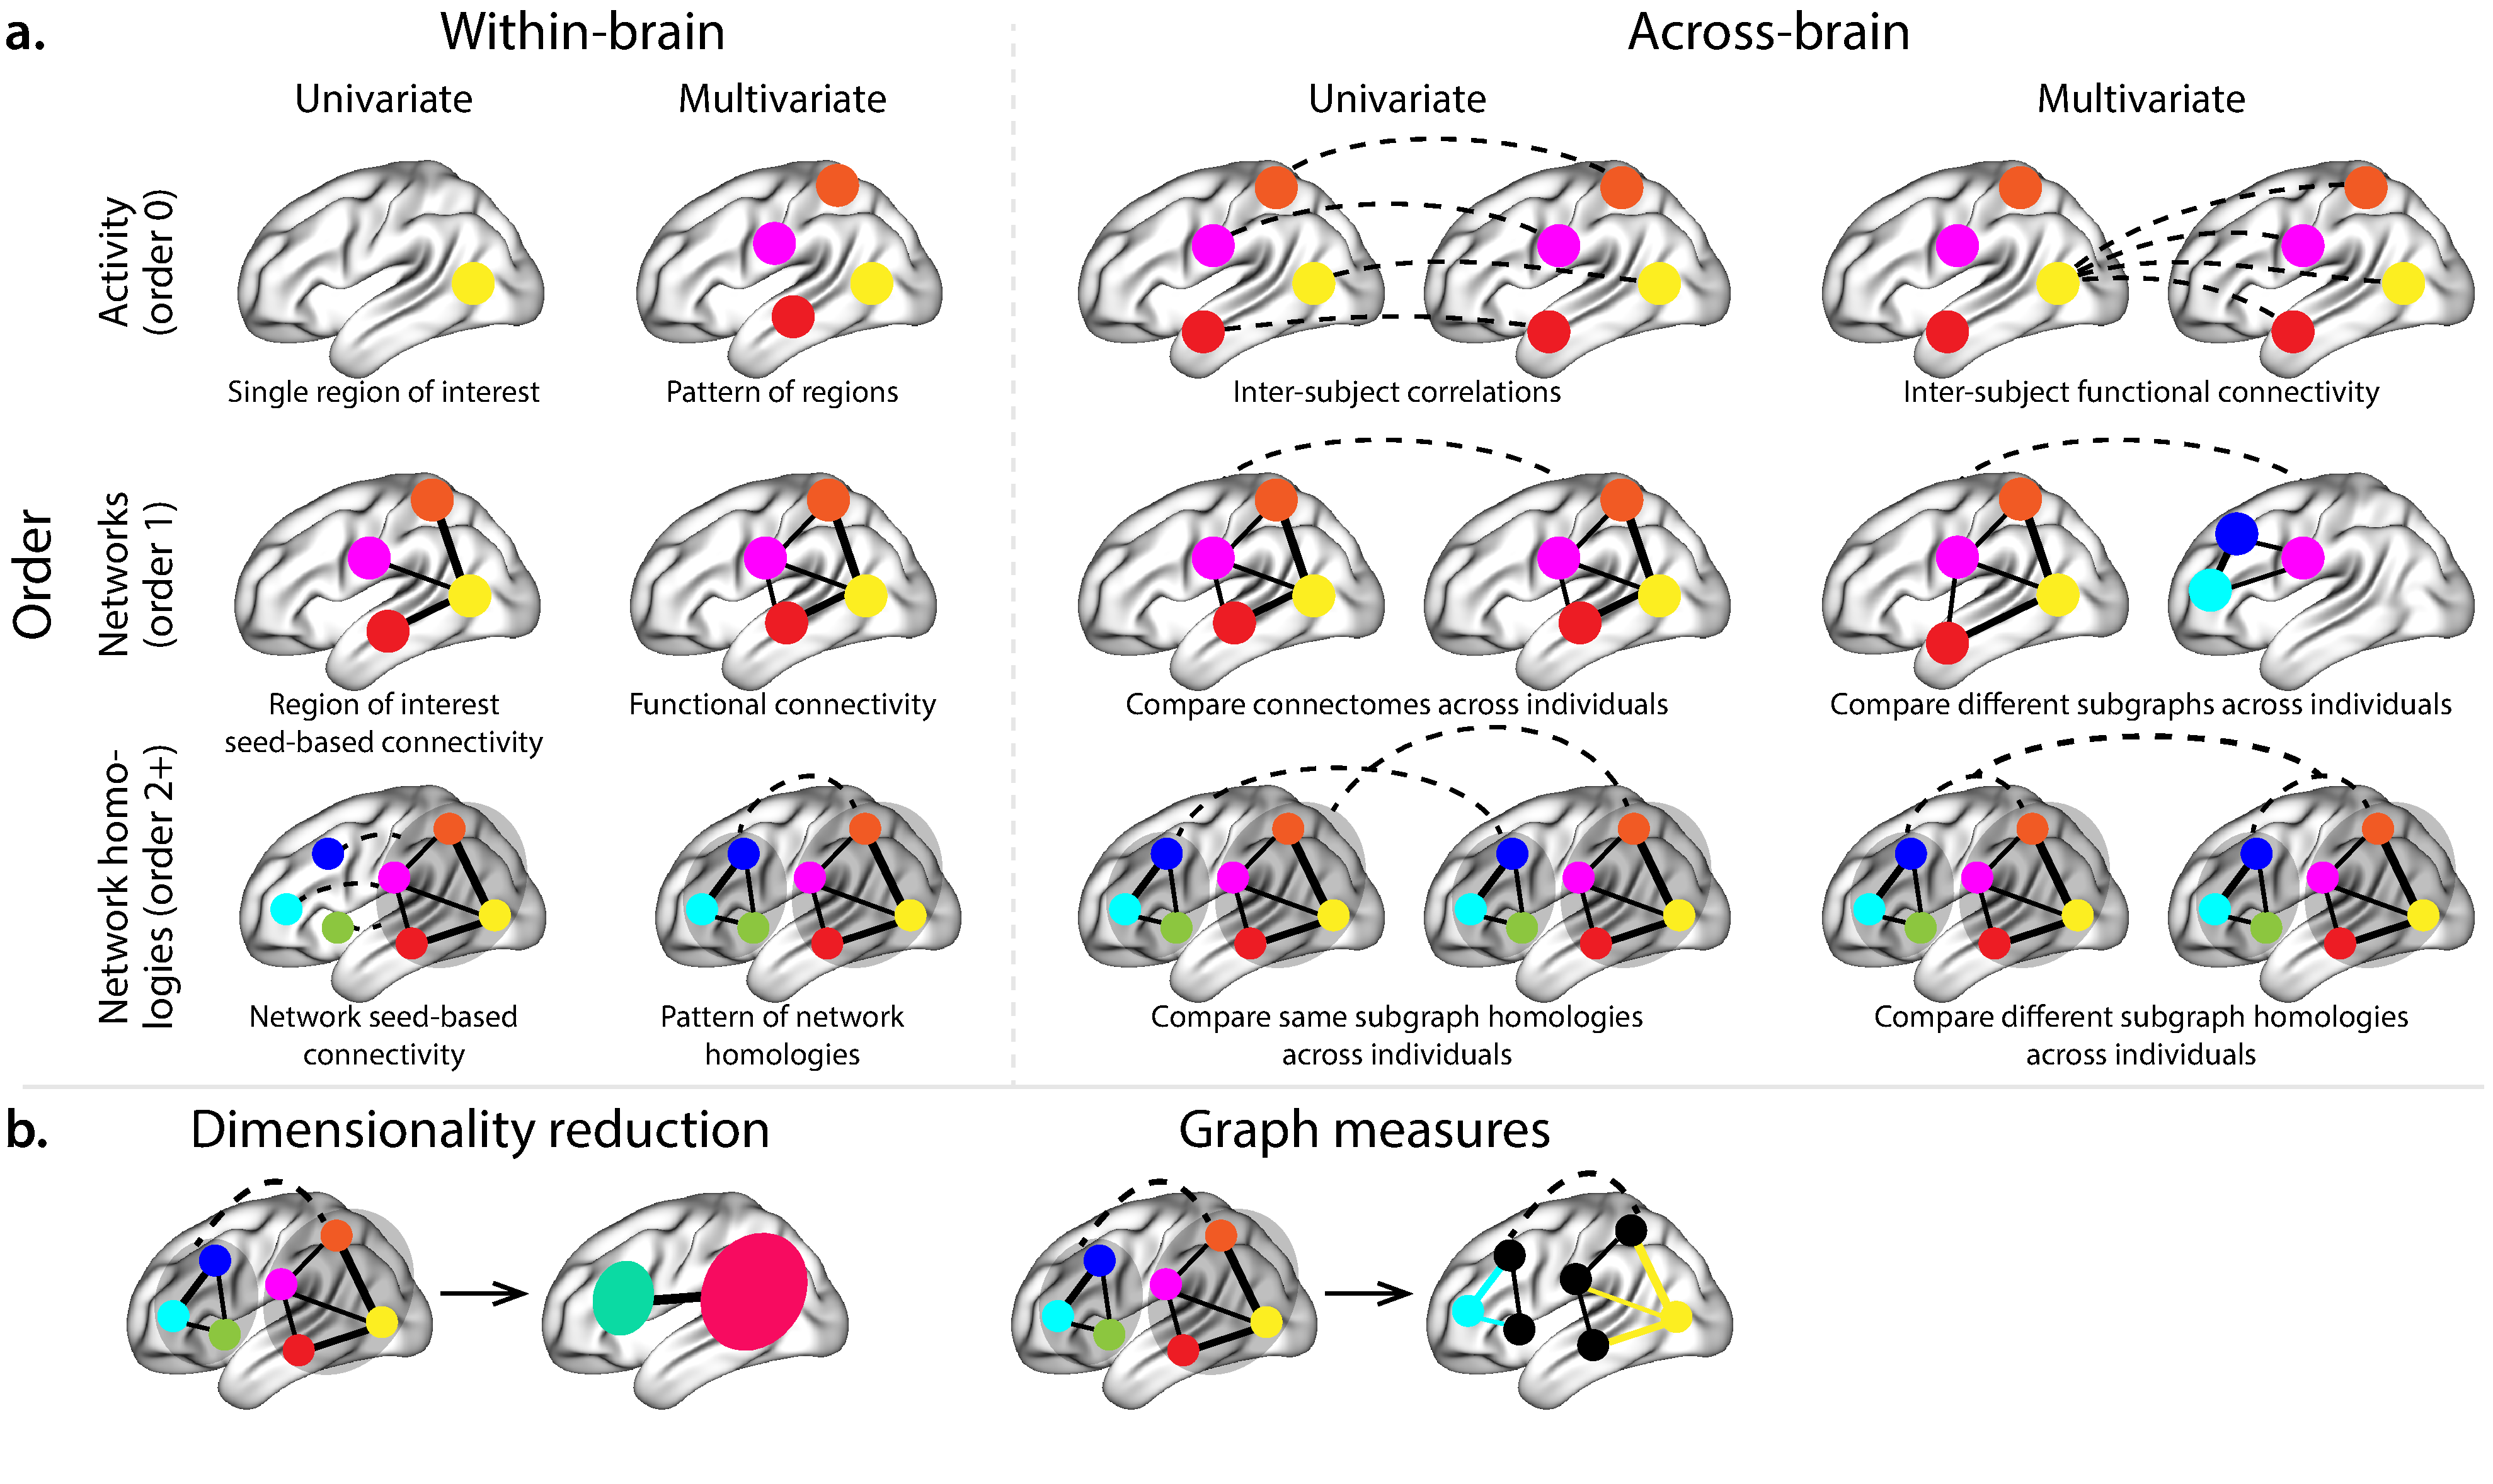
\includegraphics[width=\textwidth]{figs/patterns}
  \caption{\textbf{Neural patterns. a. A space of neural features.}
    Within-brain analyses are carried out within a single brain,
    whereas across-brain analyses compare neural patterns across two
    or more individuals' brains.  Univariate analyses characterize the
    activities of individual units (e.g., nodes, small networks,
    hierarchies of networks, etc.), whereas multivariate analyses
    characterize the patterns of activity across units.  Order 0
    patterns involve individual nodes; order 1 patterns involve
    node-node interactions; order 2 (and higher) patterns relate to
    interactions between homologous networks.  Each of these patterns
    may be static (e.g., averaging over time) or dynamic.
  \textbf{b. Summarizing neural patterns.} To efficiently compute
    with complex neural patterns, it can be useful to characterize the
    patterns using summary measures.  Dimensionality reduction
    algorithms project the patterns onto lower-dimensional spaces
    whose dimensions reflect weighted combinations or non-linear
    transformations of the dimensions in the original space.  Graph
    measures characterize each unit's participation in its associated
    network.}
  \label{fig:patterns}

\end{figure}

Studies of the neural code to date have primarily focused on
univariate or multivariate neural patterns~\DIFdelbegin \DIFdel{\mbox{%DIFAUXCMD
\citep[for review
see][]{NormEtal06b}}\hspace{0pt}%DIFAUXCMD
}\DIFdelend \DIFaddbegin \DIFadd{\mbox{%DIFAUXCMD
\cite{NormEtal06b}}\hspace{0pt}%DIFAUXCMD
}\DIFaddend , or (more recently) on patterns of dynamic
first-order correlations \DIFdelbegin \DIFdel{~\mbox{%DIFAUXCMD
\citep[i.e., interactions between pairs of
brain structures;][]{MannEtal18, FongEtal19, LuriEtal18, PretEtal17,
  ZouEtal19, DemeEtal19}}\hspace{0pt}%DIFAUXCMD
}\DIFdelend \DIFaddbegin \DIFadd{(i.e., interactions between pairs of
brain structures~\mbox{%DIFAUXCMD
\cite{MannEtal18, FongEtal19, LuriEtal18, PretEtal17,
  ZouEtal19, DemeEtal19}}\hspace{0pt}%DIFAUXCMD
)}\DIFaddend .  What might the future of this line of work
hold?  For example, is the neural code implemented through
higher-order interactions between brain structures~\DIFdelbegin \DIFdel{\mbox{%DIFAUXCMD
\citep[e.g.,
see][]{ReimEtal17}}\hspace{0pt}%DIFAUXCMD
}\DIFdelend \DIFaddbegin \DIFadd{\mbox{%DIFAUXCMD
\cite{ReimEtal17}}\hspace{0pt}%DIFAUXCMD
}\DIFaddend ?  Second-order correlations reflect
\DIFdelbegin \textit{\DIFdel{homologous}} %DIFAUXCMD
\DIFdelend \DIFaddbegin \DIFadd{homologous }\DIFaddend patterns of correlation.  In other words, if the
dynamic patterns of correlations between two regions, $A$ and $B$, are
similar to those between two other regions, $C$ and $D$, this would be
reflected in the second-order correlations between ($A$--$B$) and
($C$--$D$).  In this way, second-order correlations identify
similarities and differences between subgraphs of the brain's
connectome.  Analogously, third-order correlations reflect homologies
between second-order correlations-- i.e., homologous patterns of
homologous interactions between brain regions.  More generally,
higher-order correlations reflect homologies between patterns of
lower-order correlations.  We can then ask: which ``orders'' of
interaction are most reflective of high-level cognitive processes?

One reason one might expect to see homologous networks in a dataset is
related to the notion that network dynamics reflect ongoing neural
computations or cognitive processing~\DIFdelbegin \DIFdel{\mbox{%DIFAUXCMD
\citep[e.g.,][]{BeatEtal16}}\hspace{0pt}%DIFAUXCMD
}\DIFdelend \DIFaddbegin \DIFadd{\mbox{%DIFAUXCMD
\cite{BeatEtal16}}\hspace{0pt}%DIFAUXCMD
}\DIFaddend .  If
the nodes in two brain networks are interacting (within each network)
in similar ways then, according to our characterization of network
dynamics, we refer to the similarities between those patterns of
interaction as higher-order correlations.  When higher-order
correlations are themselves changing over time, we can also attempt to
capture and characterize those high-order dynamics.

Another central question pertains to the extent to which the neural
code is carried by activity patterns that directly reflect ongoing
cognition~\DIFdelbegin \DIFdel{\mbox{%DIFAUXCMD
\citep[e.g., following][]{HaxbEtal01, NormEtal06b}}\hspace{0pt}%DIFAUXCMD
}\DIFdelend \DIFaddbegin \DIFadd{\mbox{%DIFAUXCMD
\cite{HaxbEtal01, NormEtal06b}}\hspace{0pt}%DIFAUXCMD
}\DIFaddend , versus
the dynamic properties of the network structure itself, independent of
specific activity patterns in any given set of regions~\DIFdelbegin \DIFdel{\mbox{%DIFAUXCMD
\citep[e.g.,
following][]{BassEtal06}}\hspace{0pt}%DIFAUXCMD
}\DIFdelend \DIFaddbegin \DIFadd{\mbox{%DIFAUXCMD
\cite{BassEtal06}}\hspace{0pt}%DIFAUXCMD
}\DIFaddend .  For example, graph measures such as
centrality and degree~\DIFdelbegin \DIFdel{\mbox{%DIFAUXCMD
\citep{BullSpor09} }\hspace{0pt}%DIFAUXCMD
}\DIFdelend \DIFaddbegin \DIFadd{\mbox{%DIFAUXCMD
\cite{BullSpor09} }\hspace{0pt}%DIFAUXCMD
}\DIFaddend may be used to estimate how a
given brain structure is ``communicating'' with other structures,
independently of the specific neural representations carried by those
structures.  If one considers a brain region's position in the network
(e.g., its eigenvector centrality) as a dynamic property, one can
compare how the positions of different regions are correlated, and/or
how those patterns of correlations change over time.  We can also
compute higher-order patterns in these correlations to characterize
homologous subgraphs in the connectome that display similar changes in
their constituent brain structures' interactions with the rest of the
brain.

To gain insights into the above aspects of the neural code, we
developed a computational framework for estimating dynamic high-order
correlations in timeseries data. This framework provides an important
advance, in that it enables us to examine patterns of higher-order
correlations that are computationally intractable to estimate via
conventional methods.  Given a multivariate timeseries, our framework
provides timepoint-by-timepoint estimates of the first-order
correlations, second-order correlations, and so on.  Our approach
combines a kernel-based method for computing dynamic correlations in
timeseries data with a dimensionality reduction step
(Fig.~\ref{fig:patterns}b) that projects the resulting dynamic
correlations into a low-dimensional space.  We explored two
dimensionality reduction approaches: principle components
analysis~\DIFdelbegin \DIFdel{\mbox{%DIFAUXCMD
\citep[PCA;][]{Pear01}}\hspace{0pt}%DIFAUXCMD
}\DIFdelend \DIFaddbegin \DIFadd{\mbox{%DIFAUXCMD
\cite{Pear01} }\hspace{0pt}%DIFAUXCMD
(PCA)}\DIFaddend , which preserves an approximately
invertible transformation back to the original data~\DIFdelbegin \DIFdel{\mbox{%DIFAUXCMD
\citep[e.g., this
follows related approaches taken by][]{McInJirs19, TokeSomm19,
  GonzEtal19}}\hspace{0pt}%DIFAUXCMD
; }\DIFdelend \DIFaddbegin \DIFadd{\mbox{%DIFAUXCMD
\cite{McInJirs19, TokeSomm19,
  GonzEtal19}}\hspace{0pt}%DIFAUXCMD
, }\DIFaddend and a second non-invertible algorithm for computing
dynamic patterns in eigenvector centrality~\DIFdelbegin \DIFdel{\mbox{%DIFAUXCMD
\citep{Land95}}\hspace{0pt}%DIFAUXCMD
}\DIFdelend \DIFaddbegin \DIFadd{\mbox{%DIFAUXCMD
\cite{Land95}}\hspace{0pt}%DIFAUXCMD
}\DIFaddend .  This
latter approach characterizes correlations between each feature
dimension's relative \DIFdelbegin \textit{\DIFdel{position}} %DIFAUXCMD
\DIFdelend \DIFaddbegin \DIFadd{position }\DIFaddend in the network (at each moment
in time) in favor of the specific activity histories of different
features~\DIFdelbegin \DIFdel{\mbox{%DIFAUXCMD
\citep[also see][]{BetzEtal19, SizeEtal18, ReimEtal17}}\hspace{0pt}%DIFAUXCMD
}\DIFdelend \DIFaddbegin \DIFadd{\mbox{%DIFAUXCMD
\cite{BetzEtal19, SizeEtal18, ReimEtal17}}\hspace{0pt}%DIFAUXCMD
}\DIFaddend .

We validated our approach using synthetic data where the underlying
correlations were known.  We then applied our framework to a
neuroimaging dataset collected as participants listened to either an
audio recording of a ten-minute story, listened to a temporally
scrambled version of the story, or underwent a resting state
scan~\DIFdelbegin \DIFdel{\mbox{%DIFAUXCMD
\citep{SimoEtal16}}\hspace{0pt}%DIFAUXCMD
}\DIFdelend \DIFaddbegin \DIFadd{\mbox{%DIFAUXCMD
\cite{SimoEtal16}}\hspace{0pt}%DIFAUXCMD
}\DIFaddend .  Temporal scrambling has been used in a
growing number of studies, largely by Uri Hasson's group, to identify
brain regions that are sensitive to higher-order and longer-timescale
information (e.g., cross-sensory integration, rich narrative meaning,
complex situations, etc.) versus regions that are primarily sensitive
to low-order (e.g., sensory) information.  For example,
\cite{HassEtal08} argues that when brain areas are sensitive to fine
versus coarse temporal scrambling, this indicates that they are
``higher order'' in the sense that they process contextual information
pertaining to further-away timepoints.  By contrast, low-level
regions, such as primary sensory cortices, do not meaningfully change
their responses (after correcting for presentation order) even when
the stimulus is scrambled at fine timescales.

We used a subset of the story listening and rest data to train
across-participant classifiers to decode listening times (of groups of
participants) using a blend of neural features (comprising neural
activity patterns, as well as different orders of dynamic correlations
between those patterns that were inferred using our computational
framework).  We found that both the PCA-based and eigenvector
centrality-based approaches yielded neural patterns that could be used
to decode accurately (i.e., well above chance).  Both approaches also
yielded the best decoding accuracy for data collected during (intact)
story listening when high-order (PCA: second-order; eigenvector
centrality: fourth-order) dynamic correlation patterns were included
as features.  When we trained classifiers on the scrambled stories or
resting state data, only (relatively) lower-order dynamic patterns
were informative to the decoders.  Taken together, our results
indicate that high-level cognition is supported by high-order dynamic
patterns of communication between brain structures.




\section*{Results}
We sought to understand whether high-level cognition is reflected in
dynamic patterns of high-order correlations.  To that end, we
developed a computational framework for estimating the dynamics of
stimulus-driven high-order correlations in multivariate timeseries
data (see \DIFdelbegin \textit{\DIFdel{Dynamic inter-subject functional connectivity
  (DISFC)}} %DIFAUXCMD
\DIFdel{and }\textit{\DIFdel{Dynamic higher-order correlations}}%DIFAUXCMD
\DIFdelend \DIFaddbegin \DIFadd{Dynamic inter-subject functional connectivity
  (DISFC) and Dynamic higher-order correlations}\DIFaddend ).  We
evaluated the efficacy of this framework at recovering known patterns
in several synthetic datasets (see \DIFdelbegin \textit{\DIFdel{Synthetic data: simulating
  dynamic first-order correlations}} %DIFAUXCMD
\DIFdel{and }\textit{\DIFdel{Synthetic data:
  simulating dynamic higher-order correlations}}%DIFAUXCMD
\DIFdelend \DIFaddbegin \DIFadd{Synthetic data: simulating
  dynamic first-order correlations and Synthetic data:
  simulating dynamic higher-order correlations}\DIFaddend ).  We then
applied the framework to a public fMRI dataset collected as
participants listened to an auditorily presented story, listened to a
temporally scrambled version of the story, or underwent a resting
state scan (see \DIFdelbegin \textit{\DIFdel{Functional neuroimaging data collected during
  story listening}}%DIFAUXCMD
\DIFdelend \DIFaddbegin \DIFadd{Functional neuroimaging data collected during
  story listening}\DIFaddend ).  We used the relative decoding accuracies of
classifiers trained on different sets of neural features to estimate
which types of features reflected ongoing cognitive processing.


\subsection*{Recovering known dynamic \DIFaddbegin \DIFadd{first-order }\DIFaddend correlations\DIFdelbegin \DIFdel{from synthetic
  data}\DIFdelend }
\DIFdelbegin \subsubsection*{\DIFdel{Recovering dynamic first-order correlations}}
%DIFAUXCMD
\DIFdelend We generated synthetic datasets that differed in how the underlying first-order
correlations changed over time.  For each dataset, we applied
Equation~\ref{eqn:timecorr} with a variety of kernel shapes and
widths.  We assessed how well the true underlying correlations at each
timepoint matched the recovered correlations
(Fig.~\ref{fig:synthetic}).  For every kernel and dataset we tested,
our approach recovered the correlation dynamics we embedded into the
data.  However, the quality of these recoveries varied across
different synthetic datasets in a kernel-dependent way.



\begin{figure}
[tp]
  \centering
  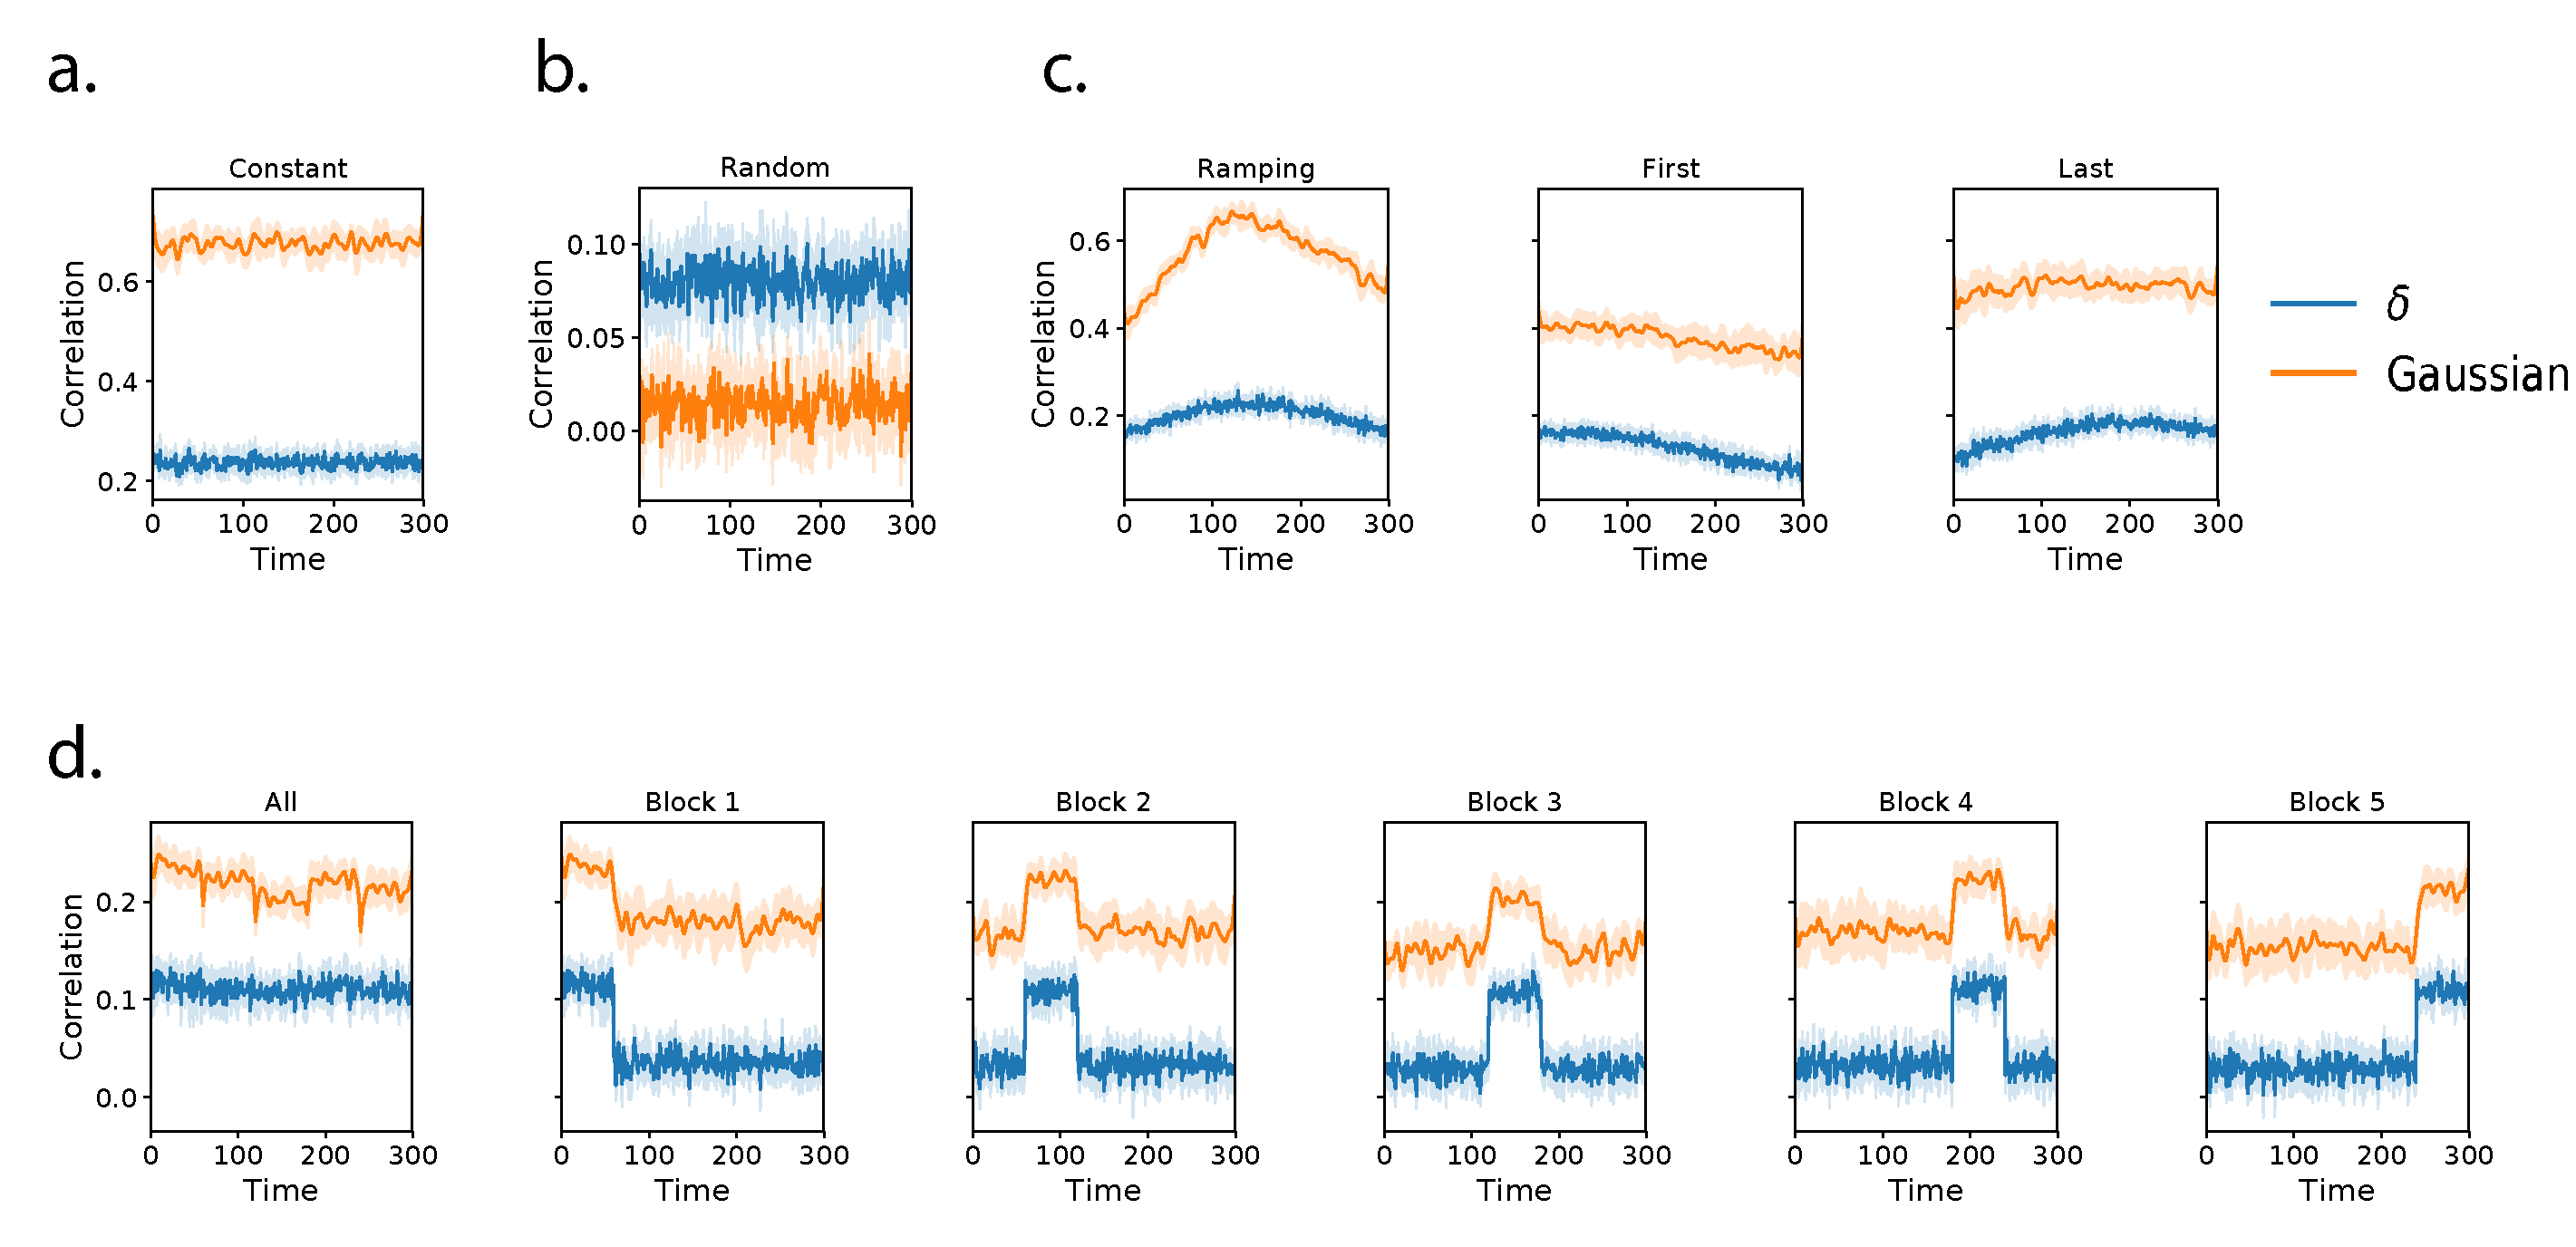
\includegraphics[width=\textwidth]{figs/synthetic_data}
  \caption{\textbf{Recovering known dynamic first-order correlations
       from synthetic data.} Each panel displays the average
    correlations between the vectorized upper triangles of the
    recovered correlation matrix at each timepoint and either the true
    underlying correlation at each timepoint or a reference
    correlation matrix.  (The averages are taken across 100 different
    randomly generated synthetic datasets of each given category, each
    with $K = 50$ features and $T = 300$ timepoints.)
    Error ribbons denote 95\% confidence intervals \DIFaddbeginFL \DIFaddFL{of the mean }\DIFaddendFL (taken across
    datasets). Different colors denote different kernel shapes, and
    the shading within each color family denotes the kernel width
    parameter.  For a complete description of each synthetic dataset,
    see \DIFdelbeginFL \textit{\DIFdelFL{Synthetic data: simulating dynamic first-order
      correlations}}%DIFAUXCMD
\DIFdelendFL \DIFaddbeginFL \DIFaddFL{Synthetic data: simulating dynamic first-order
      correlations}\DIFaddendFL . \textbf{a. Constant correlations.}  These
    datasets have a stable (unchanging) underlying correlation matrix.
  \textbf{b. Random correlations.}  These datasets are generated
    using a new independently drawn correlation matrix at each new
    timepoint. \textbf{c. Ramping correlations.} These datasets are
    generated by smoothly varying the underlying correlations between
    the randomly drawn correlation matrices at the first and last
    timepoints.  The left panel displays the correlations between the
    recovered dynamic correlations and the underlying ground truth
    correlations.  The middle panel compares the recovered
    correlations with the \DIFdelbeginFL \textit{\DIFdelFL{first}} %DIFAUXCMD
\DIFdelendFL \DIFaddbeginFL \DIFaddFL{first }\DIFaddendFL timepoint's correlation
    matrix.  The right panel compares the recovered correlations with
    the \DIFdelbeginFL \textit{\DIFdelFL{last}} %DIFAUXCMD
\DIFdelendFL \DIFaddbeginFL \DIFaddFL{last }\DIFaddendFL timepoint's correlation matrix.
  \textbf{d. Event-based correlations.} These datasets are each
    generated using five randomly drawn correlation matrices that each
    remain stable for a fifth of the total timecourse.  The left panel
    displays the correlations between the recovered dynamic
    correlations and the underlying ground truth correlations.  The
    right panels compare the recovered correlations with the
    correlation matrices unique to each event.  The vertical lines
    denote event boundaries. \DIFaddbeginFL \DIFaddFL{Source data are provided as a Source Data file.}\DIFaddendFL }
  \label{fig:synthetic}

\end{figure}

In general, wide monotonic kernel shapes (Laplace, Gaussian), and
wider kernels (within a shape), performed best when the correlations
varied gradually from moment-to-moment (Figs.~\ref{fig:synthetic}a, c,
and d).  In the extreme, as the rate of change in correlations
approaches 0 (Fig.~\ref{fig:synthetic}a), an infinitely wide kernel
would exactly recover the Pearson's correlation (e.g., compare
Eqns.~\ref{eqn:corr} and \ref{eqn:timecorr}).

When the correlation dynamics were unstructured in time
(Fig.~\ref{fig:synthetic}b), a Dirac $\delta$ kernel (infinitely
narrow) performed best.  This is because, when every timepoint's
correlations are independent \DIFdelbegin \DIFdel{from }\DIFdelend \DIFaddbegin \DIFadd{of }\DIFaddend the correlations at every other
timepoint, averaging data over time dilutes the available signal.
Following a similar pattern, holding kernel shape fixed, narrower
kernel parameters better recovered randomly varying correlations.

\DIFdelbegin \subsubsection*{\DIFdel{Recovering dynamic higher-order correlations}}
%DIFAUXCMD
\DIFdelend \DIFaddbegin \subsection*{\DIFadd{Recovering known dynamic higher-order correlations}}
\DIFaddend Following our approach to evaluating our ability to recover known
dynamic first-order correlations from synthetic data, we generated an
analogous second set of synthetic datasets that we designed to exhibit
known dynamic first-order \DIFdelbegin \textit{\DIFdel{and}} %DIFAUXCMD
\DIFdelend \DIFaddbegin \DIFadd{and }\DIFaddend second-order correlations (see
\DIFdelbegin \textit{\DIFdel{Synthetic data: simulating dynamic higher-order
  correlations}}%DIFAUXCMD
\DIFdelend \DIFaddbegin \DIFadd{Synthetic data: simulating dynamic higher-order
  correlations}\DIFaddend ).  We generated a total of 400 datasets \DIFaddbegin \DIFadd{(100 datasets
for each category) }\DIFaddend that varied in
how the first-order and second-order correlations changed over time.
We then repeatedly applied Equation~\ref{eqn:timecorr} using the
overall best-performing kernel from our first-order tests (a Laplace
kernel with a width of 20; Fig.~\ref{fig:synthetic}) to assess how
closely the recovered dynamic correlations matched the dynamic
correlations we had embedded into the datasets.

Overall, we found that we could reliably recover both first-order and
second-order correlations from the synthetic data
(Fig.~\ref{fig:higher_order_sims}).  When the correlations were stable
for longer intervals, or changed gradually (constant, ramping, and
event datasets), recovery performance was relatively high, and we were
better able to recover dynamic first-order correlations than
second-order correlations.  This is because errors in our \DIFdelbegin \textit{\DIFdel{estimation}}
%DIFAUXCMD
\DIFdelend \DIFaddbegin \DIFadd{estimation
}\DIFaddend procedure at lower orders necessarily propagate to higher orders
(since lower-order correlations are used to estimate higher-order
correlations).  Conversely, when the correlations were particularly
\DIFdelbegin \textit{\DIFdel{un}}%DIFAUXCMD
\DIFdel{stable }\DIFdelend \DIFaddbegin \DIFadd{unstable }\DIFaddend (random datasets), we better recovered second-order
correlations.  This is because noise in our \DIFdelbegin \textit{\DIFdel{data generation}}
%DIFAUXCMD
\DIFdelend \DIFaddbegin \DIFadd{data generation
}\DIFaddend procedure propagates from higher orders to lower orders (see
\DIFdelbegin \textit{\DIFdel{Synthetic data: simulating dynamic high-order correlations}}%DIFAUXCMD
\DIFdelend \DIFaddbegin \DIFadd{Synthetic data: simulating dynamic high-order correlations}\DIFaddend ).


\begin{figure}
[tp]
  \centering
  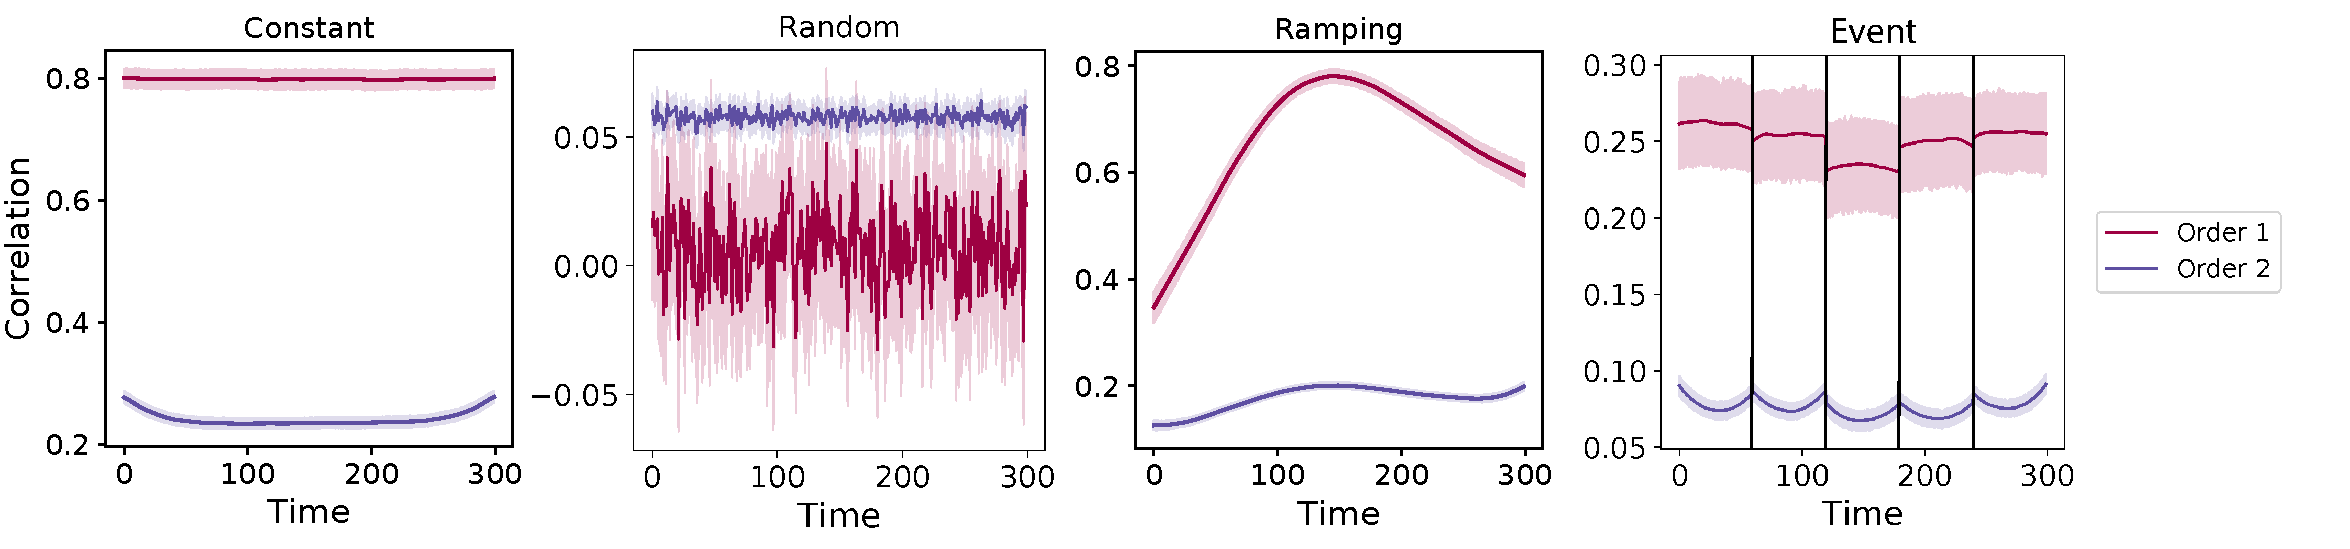
\includegraphics[width=\textwidth]{figs/higher_order_sims}
  \caption{\textbf{Recovery of simulated first-order and second-order dynamic correlations.} Each panel displays the average correlations
    between the vectorized upper triangles of the recovered
    first-order and second-order correlation matrices and the true
    (simulated) first-order and second order correlation matrices at each
    timepoint and for each synthetic dataset.  (The averages are taken across 100 different
    randomly generated synthetic datasets of each given category, each
    with $K = 10$ features and $T = 300$ timepoints.)
    Error ribbons denote 95\% confidence intervals \DIFaddbeginFL \DIFaddFL{of the mean }\DIFaddendFL (taken across
    datasets).  For a complete description of each synthetic dataset,
    see \DIFdelbeginFL \textit{\DIFdelFL{Synthetic data: simulating dynamic higher-order
      correlations}}%DIFAUXCMD
\DIFdelendFL \DIFaddbeginFL \DIFaddFL{Synthetic data: simulating dynamic higher-order
      correlations}\DIFaddendFL .  All estimates represented in this figure were
    computed using a Laplace kernel
    (width~$=20$).  \textbf{Constant.} These datasets
    have stable (unchanging) underlying second-order correlation
    matrices. \textbf{Random.} These datasets are
    generated using a new independently drawn second-order correlation
    matrix at each timepoint. \textbf{Ramping.}
    These datasets are generated by smoothly varying the underlying
    second-order correlations between the randomly drawn correlation
    matrices at the first and last timepoints. \textbf{Event.}  These datasets are each generated using five
    randomly drawn second-order correlation matrices that each remain
    stable for a fifth of the total timecourse.  The
    vertical lines denote event boundaries.  Note that the ``dips''
    and ``ramps'' at the boundaries of sharp transitions (e.g., the
    beginning and ends of the ``constant'' and ``ramping'' datasets,
    and at the event boundaries of the ``event'' datasets) are
    finite-sample effects that reflect the reduced numbers of samples
    that may be used to accurately estimate correlations at sharp
    boundaries. \DIFaddbeginFL \DIFaddFL{Source data are provided as a Source Data file.}\DIFaddendFL }
  \label{fig:higher_order_sims}

\end{figure}


We also examined the impact of the data duration (Fig.~\timeheatmap)
and complexity (number of zero-order features; Fig.~\features) on our
ability to accurately recover ground truth first-order and
second-order dynamic correlations.  In general, we found that our approach
better recovers ground truth dynamic correlations from longer duration
timeseries data.  We also found that our approach tends to best recover data generated
using fewer zero-order features (i.e., lower complexity), although
this tendency was not strictly monotonic.  Further, because our data
generation procedure requires $\mathcal{O}(K^{4})$ memory to generate
a second-order timeseries with $K$ zero-order features, we were not
able to fully explore how the number of zero-order features affects
recovery accuracy as the number of features gets larger (e.g., as it
approaches the number of features present in the fMRI data we examine
below).  Although we were not able to formally test this to our
satisfaction, we expect that accurately estimating dynamic high-order
correlations would require data with many more zero-order features
than we were able to simulate.  Our reasoning is that
high-order correlations necessarily involve larger numbers of
lower-order features, so achieving adequate ``resolution'' high-order
timeseries might require many low-order features.

Taken together, our explorations using synthetic data indicated that
we are able to partially, but not perfectly, recover ground truth
dynamic first-order and second-order correlations.  This suggests that
our modeling approach provides a meaningful (if noisy) estimate of
high-order correlations.  We next turned to analyses of human fMRI data
to examine whether the recovered dynamics might reflect the dynamics
of human cognition during a naturalistic story-listening task.

\subsection*{Cognitively relevant dynamic high-order correlations in
  fMRI data}
We used across-participant temporal decoders to identify cognitively
relevant neural patterns in fMRI data (see \DIFdelbegin \textit{\DIFdel{Forward inference
  and decoding accuracy}}%DIFAUXCMD
\DIFdelend \DIFaddbegin \DIFadd{Forward inference
  and decoding accuracy}\DIFaddend ).  The dataset we examined~\DIFdelbegin \DIFdel{\mbox{%DIFAUXCMD
\citep[collected
by][]{SimoEtal16} }\hspace{0pt}%DIFAUXCMD
}\DIFdelend \DIFaddbegin \DIFadd{\mbox{%DIFAUXCMD
\cite{SimoEtal16} }\hspace{0pt}%DIFAUXCMD
}\DIFaddend comprised four experimental conditions that exposed
participants to stimuli that varied systematically in how cognitively
engaging they were.  The \DIFdelbegin \textit{\DIFdel{intact}} %DIFAUXCMD
\DIFdel{experimental condition }\DIFdelend \DIFaddbegin \DIFadd{intact experimental condition (intact) }\DIFaddend had
participants listen to an audio recording of a 10-minute story.  The
\DIFdelbegin \textit{\DIFdel{paragraph}}%DIFAUXCMD
\DIFdel{-scrambled experimental condition }\DIFdelend \DIFaddbegin \DIFadd{paragraph-scrambled experimental condition (paragraph) }\DIFaddend had participants
listen to a temporally scrambled version of the story, where the
paragraphs occurred out of order (but where the same total set of
paragraphs were presented over the full listening interval).  All
participants in this condition experienced the scrambled paragraphs in
the same order.  The \DIFdelbegin \textit{\DIFdel{word}}%DIFAUXCMD
\DIFdel{-scrambled experimental condition }\DIFdelend \DIFaddbegin \DIFadd{word-scrambled experimental condition (word)
}\DIFaddend had participants listen to a temporally scrambled version of the story
where the words in the story occurred in a random order.  All
participants in the word condition experienced the scrambled words in
the same order.  Finally, in a \DIFdelbegin \textit{\DIFdel{rest}} %DIFAUXCMD
\DIFdel{experimental condition }\DIFdelend \DIFaddbegin \DIFadd{rest experimental condition (rest)}\DIFaddend ,
participants lay in the scanner with no overt stimulus, with their
eyes open (blinking as needed).  This public dataset provided a convenient
means of testing our hypothesis that different levels of cognitive
processing and engagement are reflected in different orders of brain
activity dynamics.


\begin{figure}
[tp]
  \centering
  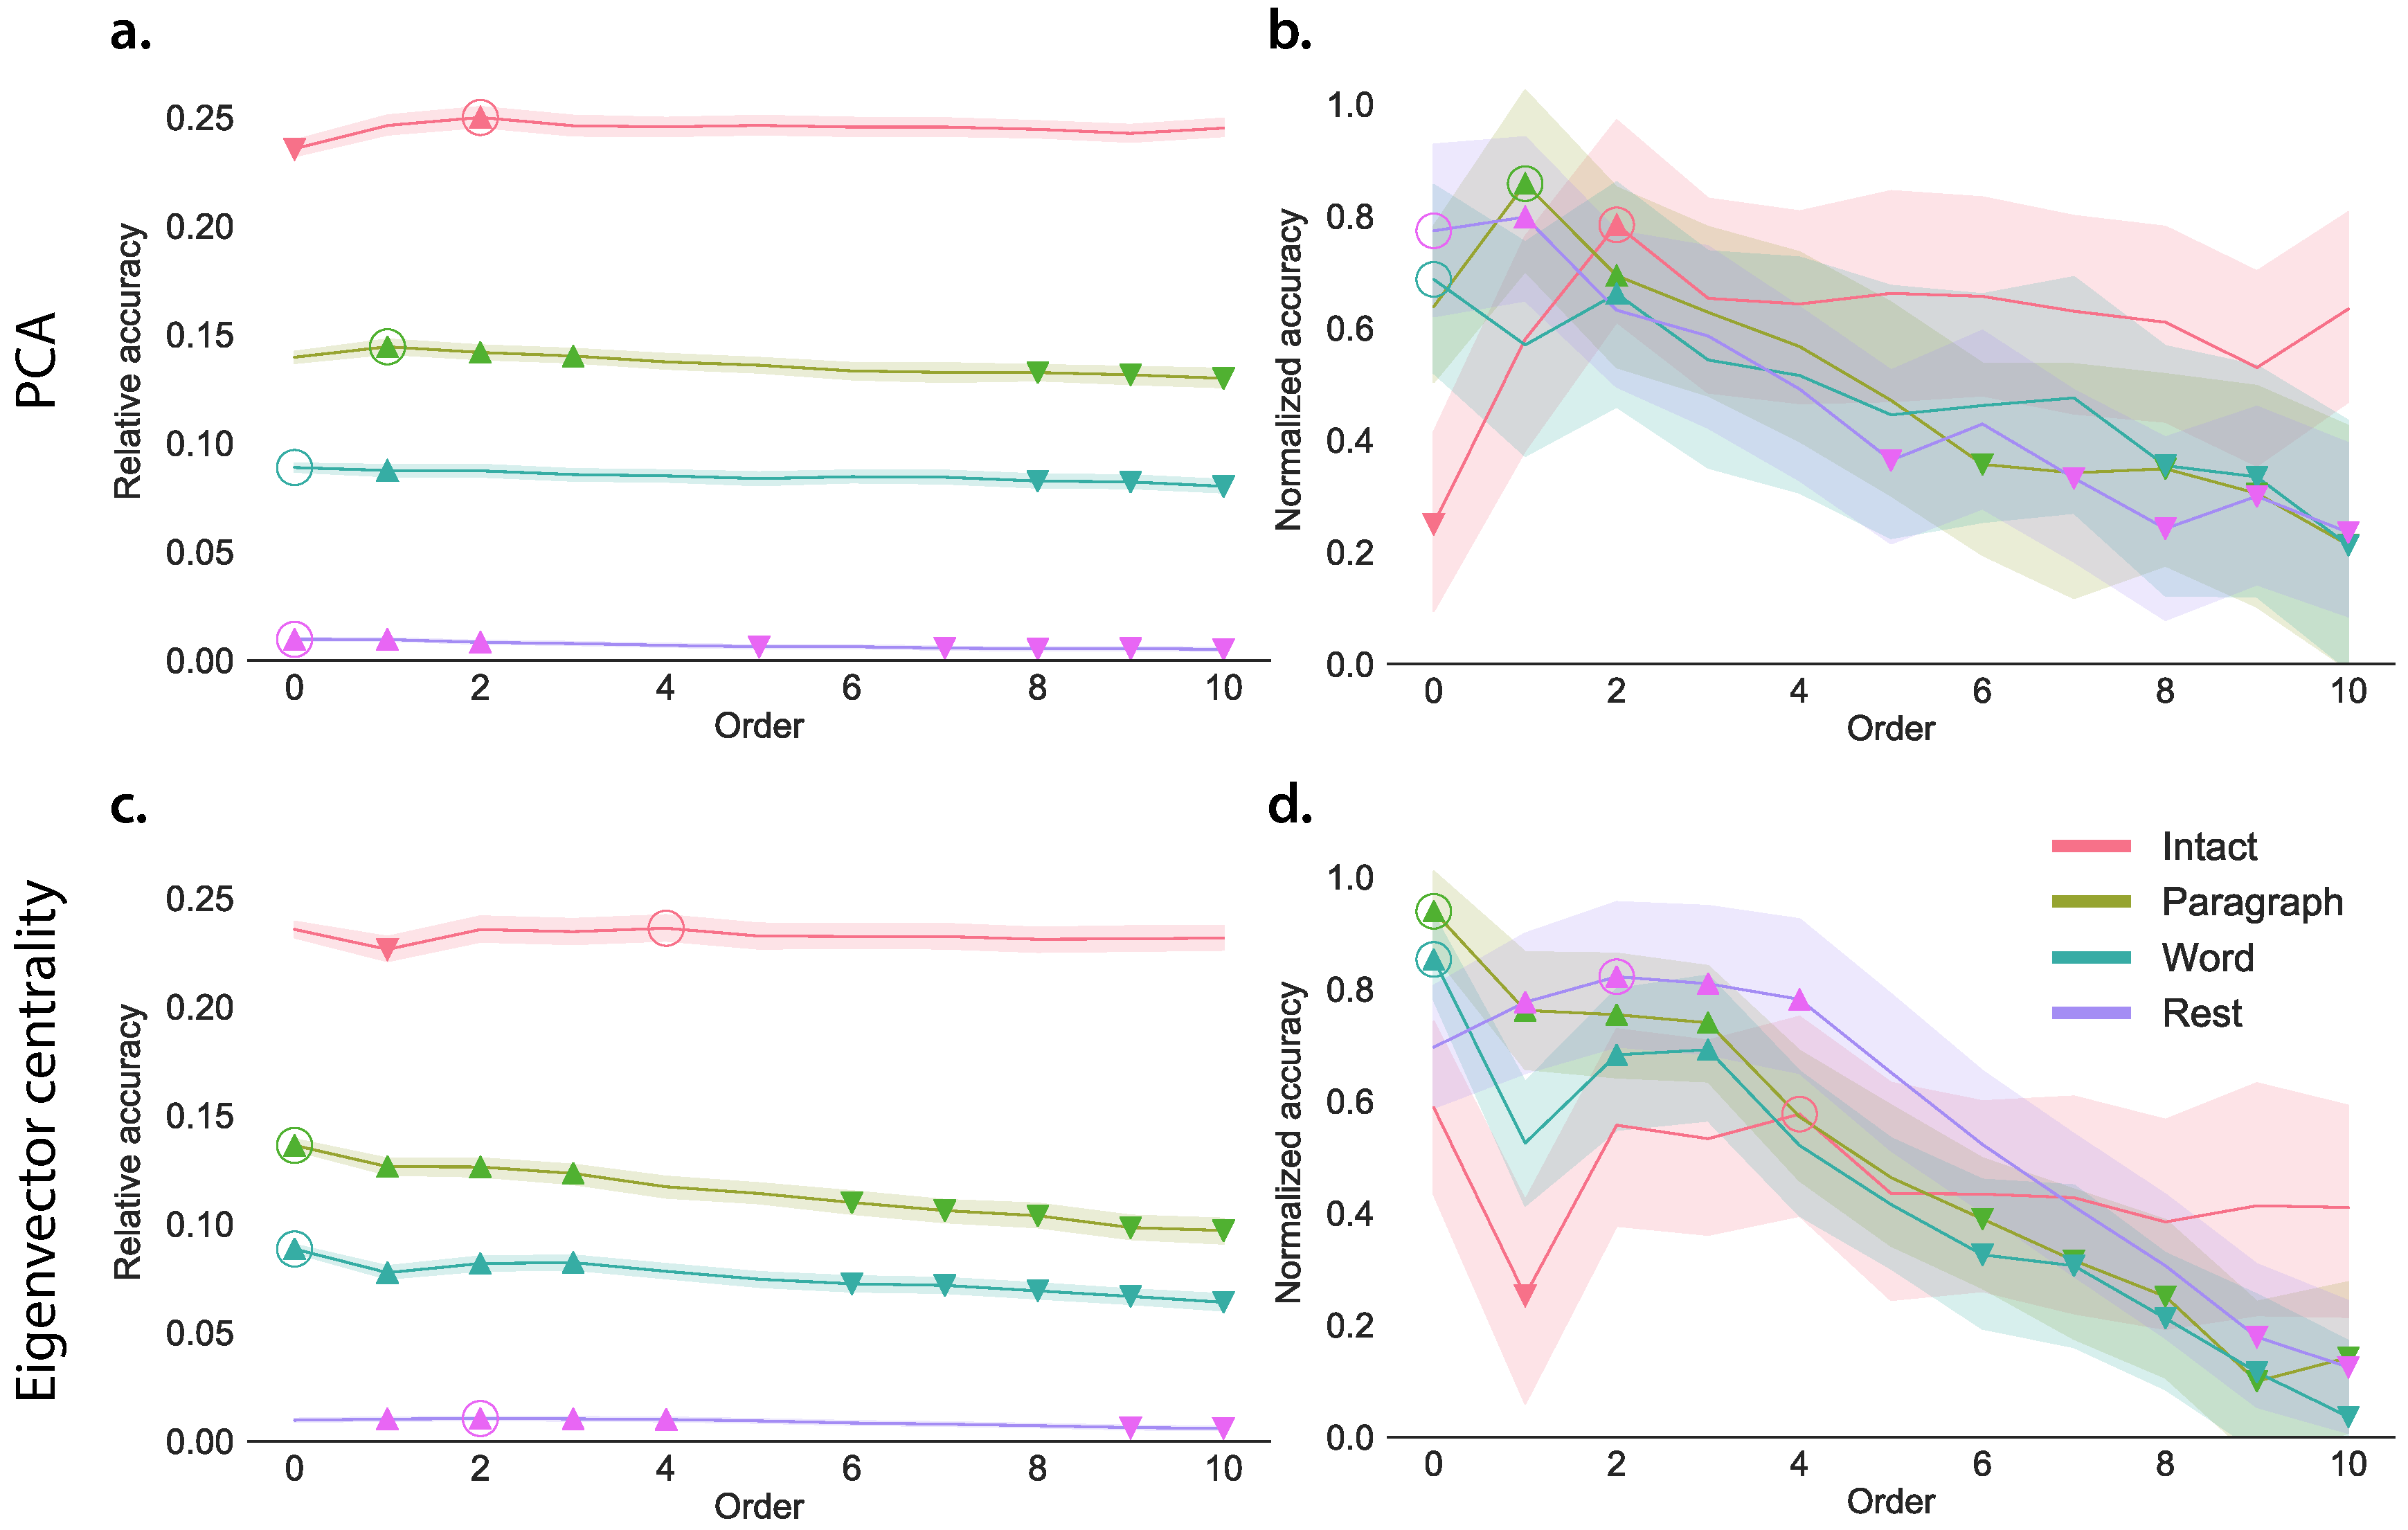
\includegraphics[width=\textwidth]{figs/decode_level}
  \caption{\textbf{Across-participant timepoint decoding accuracy varies with
       correlation order and cognitive engagement.}
     \textbf{a.~Decoding accuracy as a function of order: PCA.}
   \DIFdelbeginFL \textit{\DIFdelFL{Order}} %DIFAUXCMD
\DIFdelendFL \DIFaddbeginFL \DIFaddFL{``Order'' }\DIFaddendFL ($x$-axis) refers to the maximum order of dynamic
    correlations that were available to the classifiers (see
    \DIFdelbeginFL \textit{\DIFdelFL{Feature weighting and testing}}%DIFAUXCMD
\DIFdelendFL \DIFaddbeginFL \DIFaddFL{Feature weighting and testing}\DIFaddendFL ).  The reported
    across-participant decoding accuracies are averaged over all
    kernel shapes and widths (see \DIFdelbeginFL \textit{\DIFdelFL{Identifying robust decoding
      results}}%DIFAUXCMD
\DIFdelendFL \DIFaddbeginFL \DIFaddFL{Identifying robust decoding
      results}\DIFaddendFL ).  The $y$-values are displayed relative to chance
    accuracy (intact: $\frac{1}{300}$; paragraph: $\frac{1}{272}$;
    word: $\frac{1}{300}$; rest: $\frac{1}{400}$; these chance accuracies
    were subtracted from the observed accuracies to obtain the
    relative accuracies reported on the $y$-axis).  The error ribbons
    denote 95\% confidence intervals \DIFaddbeginFL \DIFaddFL{of the means }\DIFaddendFL across cross-validation folds
    (i.e., random assignments of participants to the training and test
    sets).  The colors denote the experimental condition.  Arrows
    denote sets of features that yielded reliably higher (upward
    facing) or lower (downward facing) decoding accuracy than the mean
    of all other features (via a two-tailed $t$-test, thresholded at
    $p < 0.05$).  Figure~\ref{fig:ttests} displays additional
    comparisons between the decoding accuracies achieved using
    different sets of neural features.  The circled values represent
    the maximum decoding accuracy within each experimental condition.
  \textbf{b.~Normalized timepoint decoding accuracy as a function of order:
       PCA.}  This panel displays the same results as Panel a, but here
    each curve has been normalized to \DIFdelbeginFL \DIFdelFL{be bounded between 0 and }\DIFdelendFL \DIFaddbeginFL \DIFaddFL{have a maximum value of }\DIFaddendFL 1 \DIFdelbeginFL \DIFdelFL{(inclusive) by subtracting the }\DIFdelendFL \DIFaddbeginFL \DIFaddFL{and a
    }\DIFaddendFL minimum \DIFdelbeginFL \DIFdelFL{accuracy
    }\DIFdelendFL \DIFaddbeginFL \DIFaddFL{value of 0 }\DIFaddendFL (\DIFdelbeginFL \DIFdelFL{across all folds and orders) and then dividing by }\DIFdelendFL \DIFaddbeginFL \DIFaddFL{including }\DIFaddendFL the \DIFdelbeginFL \DIFdelFL{maximum
    accuracy (again, across all folds }\DIFdelendFL \DIFaddbeginFL \DIFaddFL{upper }\DIFaddendFL and \DIFdelbeginFL \DIFdelFL{orders}\DIFdelendFL \DIFaddbeginFL \DIFaddFL{lower bounds of the
    respective 95\% confidence intervals of the mean}\DIFaddendFL ).  Panels a and b used PCA to
    project each high-dimensional pattern of dynamic correlations onto
    a lower-dimensional space. \textbf{c.~Timepoint decoding accuracy as a
       function of order: eigenvector centrality.} This panel is in the
    same format as Panel a, but here eigenvector centrality has been
    used to project the high-dimensional patterns of dynamic
    correlations onto a lower-dimensional space.
 \textbf{d.~Normalized timepoint decoding accuracy as a function of order:
       eigenvector centrality.}  This panel is in the same format as
    Panel b, but here eigenvector centrality has been used to project
    the high-dimensional patterns of dynamic correlations onto a
    lower-dimensional space. See
    Figures~\kernelshape~and~\kernelwidth~for decoding results broken
    down by kernel shape and width, respectively. \DIFaddbeginFL \DIFaddFL{Source data are provided as a Source Data file.}\DIFaddendFL }
  \label{fig:decoding}

\end{figure}

In brief, we computed timeseries of dynamic high-order correlations
that were similar across participants in each of two randomly assigned
groups: a training group and a test group.  We then trained
classifiers on the training group's data to match each sample from the
test group with a stimulus timepoint.  Each classifier comprised a
weighted blend of neural patterns that reflected up to
$n^\mathrm{th}$-order dynamic correlations (see \DIFdelbegin \textit{\DIFdel{Feature
  weighting and testing}}%DIFAUXCMD
\DIFdel{, Fig.~\ref{fig:pipeline}}\DIFdelend \DIFaddbegin \DIFadd{Feature
  weighting and testing}\DIFaddend ).  We repeated this process for
$n \in \left\{ 0, 1, 2, ..., 10 \right\}$.  Our examinations of
synthetic data suggested that none of the kernels we examined were
``universal'' in the sense of optimally recovering underlying
correlations regardless of the temporal structure of those
correlations.  We found a similar pattern in the (real) fMRI data,
whereby different kernels yielded different decoding accuracies, but
no single kernel emerged as the clear ``best.''  In our analyses of
neural data, we therefore averaged our decoding results over a variety
of kernel shapes and widths in order to identify results that were
robust to specific kernel parameters (see \DIFdelbegin \textit{\DIFdel{Identifying robust
  decoding results}}%DIFAUXCMD
\DIFdelend \DIFaddbegin \DIFadd{Identifying robust
  decoding results}\DIFaddend ).

Our approach to estimating dynamic high-order correlations entails
mapping the high-dimensional feature space of correlations
(represented by a $T$ by
$\mathcal{O}(K^2)$ matrix) onto a lower-dimensional feature space
(represented by a $T$ by $K$ matrix).
We carried out two sets of analyses that differed in how this mapping
was computed.  The first set of analyses used PCA to find a
low-dimensional embedding of the original dynamic correlation matrices
(Fig.~\ref{fig:decoding}a,b).  The second set of analyses
characterized correlations in dynamics of each feature's eigenvector
centrality, but did not preserve the underlying activity dynamics
(Fig.~\ref{fig:decoding}c,d).




\begin{figure}
[tp]
\centering
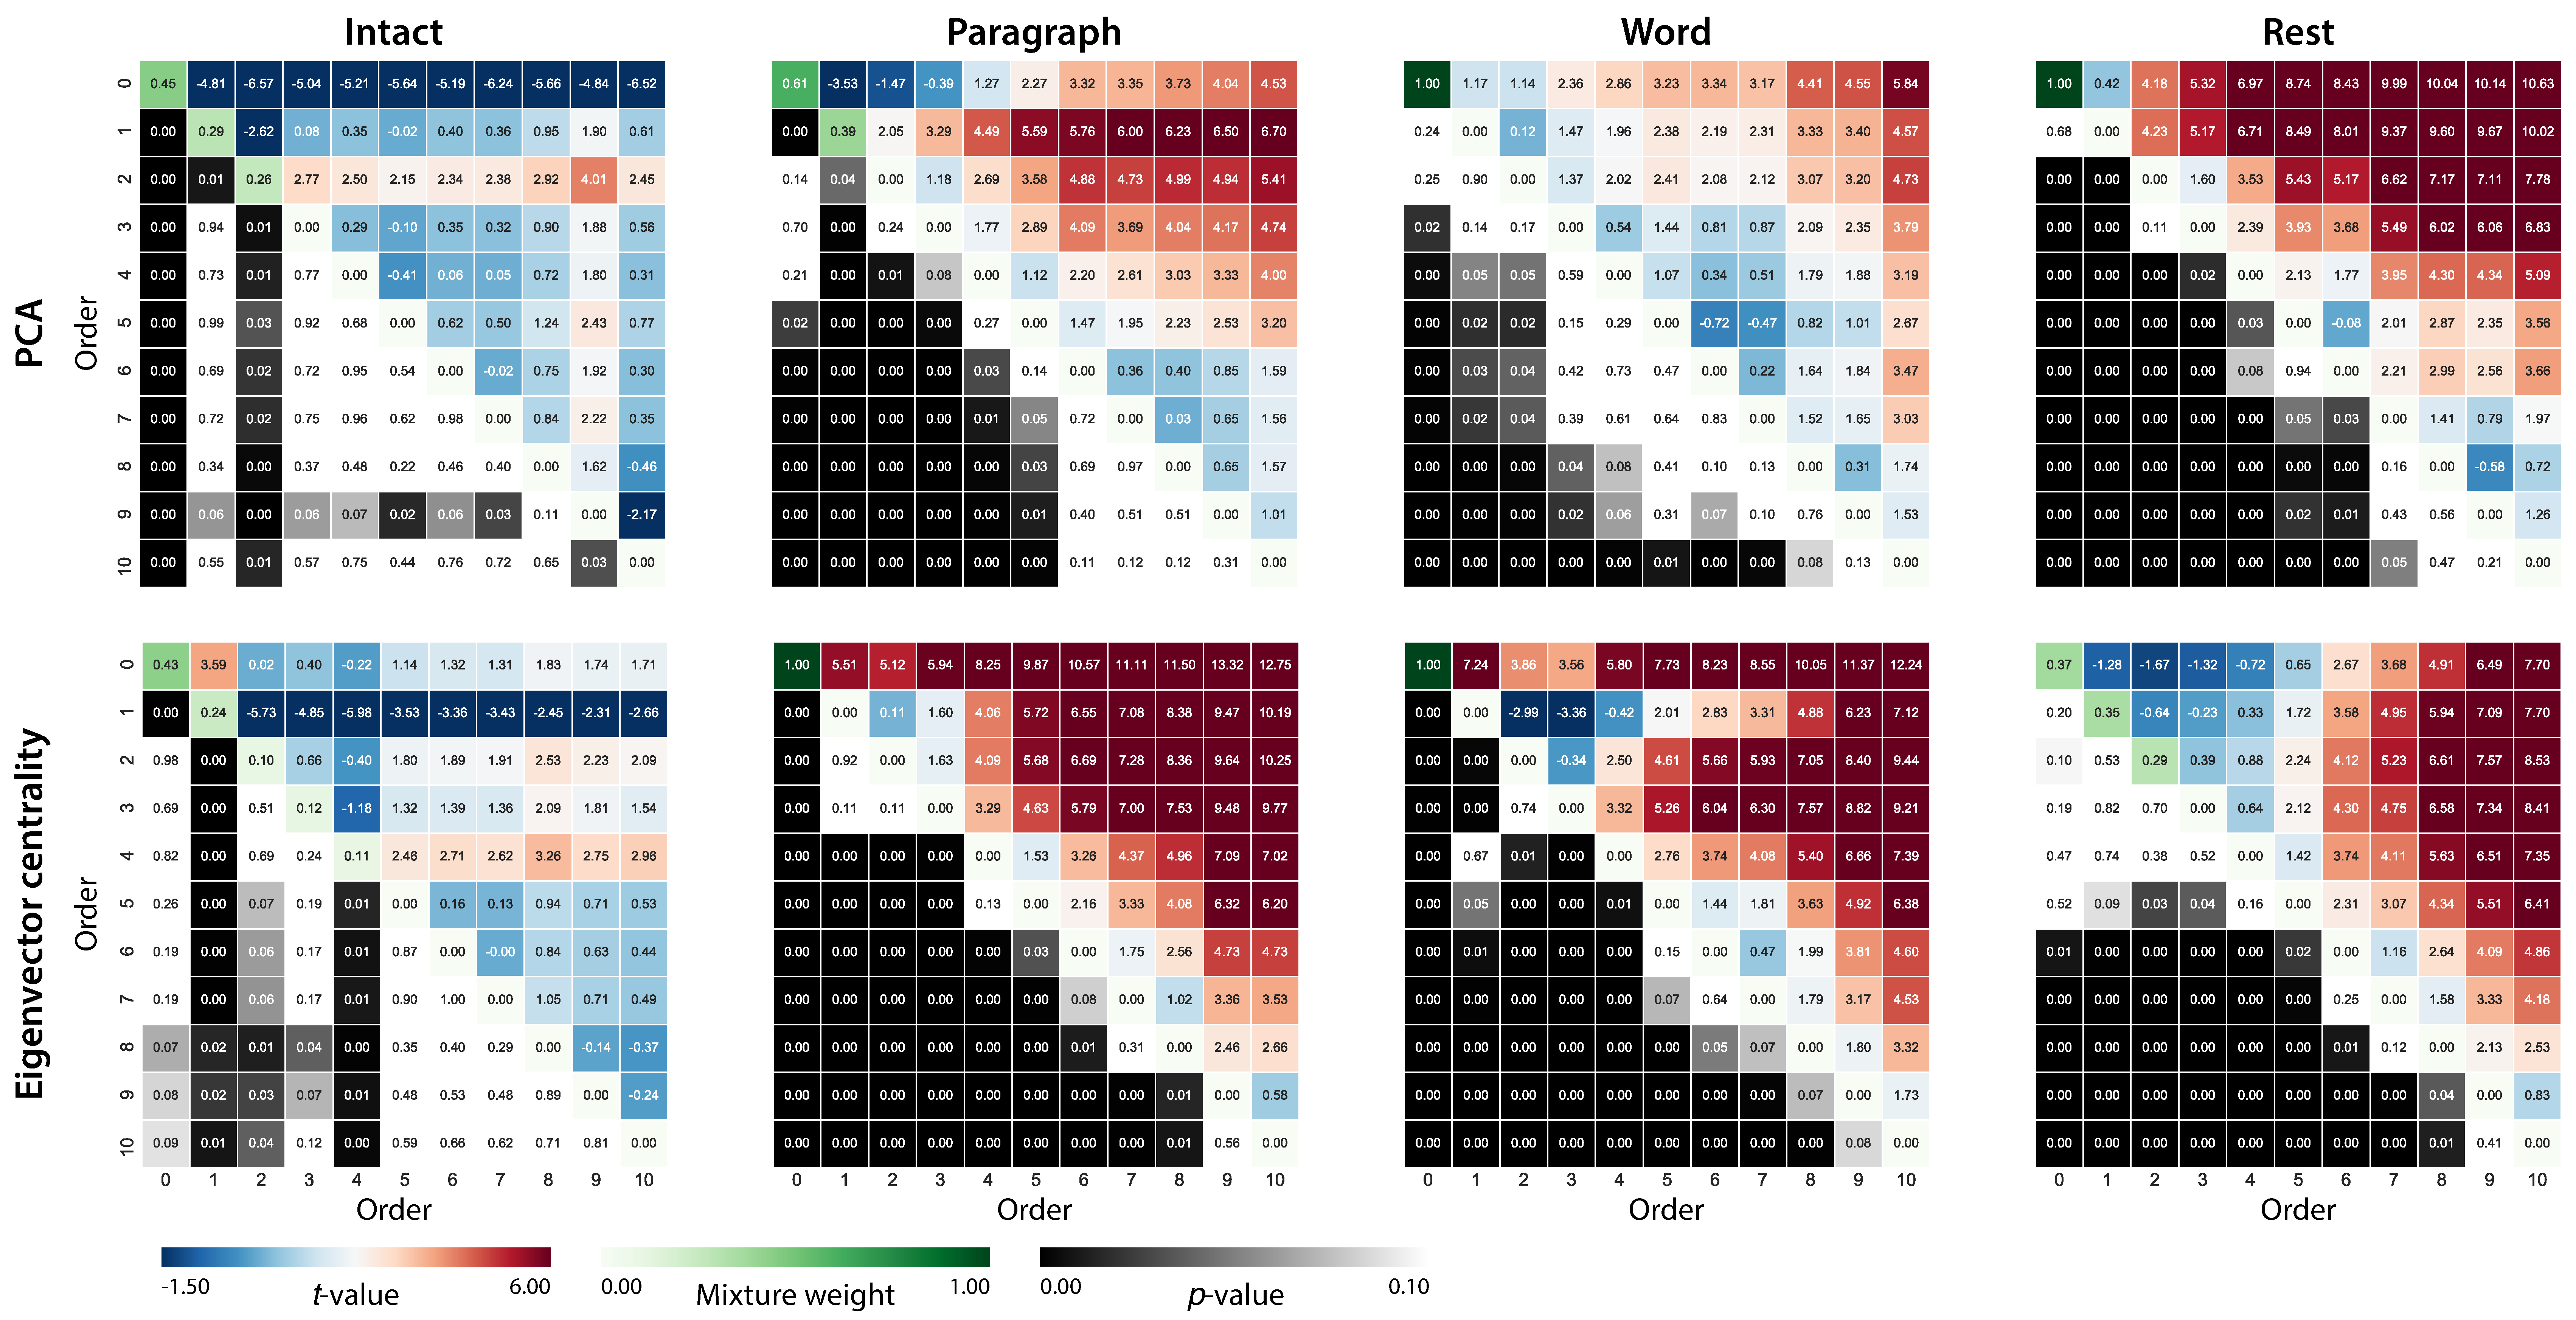
\includegraphics[width=1\textwidth]{figs/stats_heatmaps}
\caption{\textbf{Statistical summary of decoding accuracies for
     different neural features.}  Each column of matrices displays decoding
  results for one experimental condition (intact, paragraph, word, and
  rest).  We considered dynamic activity patterns (order 0) and
  dynamic correlations at different orders (order $> 0$).  We used
  two-tailed $t$-tests to compare the
  distributions of decoding accuracies obtained using each pair of
  features.  The distributions for each feature reflect the set of
  average decoding accuracies (across all kernel parameters), obtained
  for each random assignment of training and test groups.
  In the upper triangles of each matrix, warmer colors (positive $t$-values) indicate that the
  neural feature indicated in the given row yielded higher accuracy than the
  feature indicated in the given column.  Cooler colors (negative
  $t$-values) indicate that
  the feature in the given row yielded lower decoding accuracy than
  the feature in the given column.  The lower triangles of each map
  denote the corresponding $p$-values for the $t$-tests.  The diagonal
  entries display the relative average optimized weight given to each type of feature in
  a decoder that included all feature types (see \DIFdelbeginFL \textit{\DIFdelFL{Feature
    weighting and testing}}%DIFAUXCMD
\DIFdelendFL \DIFaddbeginFL \DIFaddFL{Feature
    weighting and testing}\DIFaddendFL ). \DIFaddbeginFL \DIFaddFL{Source data are provided as a Source Data file.}\DIFaddendFL }
\label{fig:ttests}
\end{figure}

Both sets of temporal decoding analyses yielded qualitatively similar
results for the auditory (non-rest) conditions of the experiment
(Fig.~\ref{fig:decoding}: pink, green, and teal lines;
Fig.~\ref{fig:ttests}: three leftmost columns).  The highest
decoding accuracy for participants who listened to the intact
(unscrambled) story was achieved using high-order dynamic correlations
(PCA: second-order; eigenvector-centrality: fourth-order).  Scrambled
versions of the story were best decoded by lower-order correlations
(PCA/paragraph: first-order; PCA/word: order zero; eigenvector
centrality/paragraph: order zero; eigenvector centrality/word: order
zero).  The two sets of analyses yielded different decoding results on
resting state data (Fig.~\ref{fig:decoding}: purple lines;
Fig.~\ref{fig:ttests}: rightmost column).  We note
that, while the resting state times could be decoded reliably, the
accuracies were only very slightly above chance.  We speculate that
the decoders might have picked up on attentional drift, boredom, or
tiredness; we hypothesize that these all increased throughout the resting
state scan.  The decoders might be picking up on aspects of these
loosely defined cognitive states that are common across individuals.
The PCA-based approach achieved the highest resting state decoding
accuracy using order zero features (non-correlational,
activation-based), whereas the eigenvector centrality-based approach
achieved the highest resting state decoding accuracy using
second-order correlations.  Taken together, these analyses indicate
that high-level cognitive processing (while listening to the intact
story) is reflected in the dynamics of high-order correlations in
brain activity, whereas lower-level cognitive processing (while
listening to scrambled versions of the story that lack rich meaning)
is reflected in the dynamics of lower-order correlations and
non-correlational activity dynamics.  Further, these patterns are
associated both with the underlying activity patterns (characterized
using PCA) and also with the changing relative positions that
different brain areas occupy in their associated networks
(characterized using eigenvector centrality).


\begin{figure}
[tp]
  \centering
  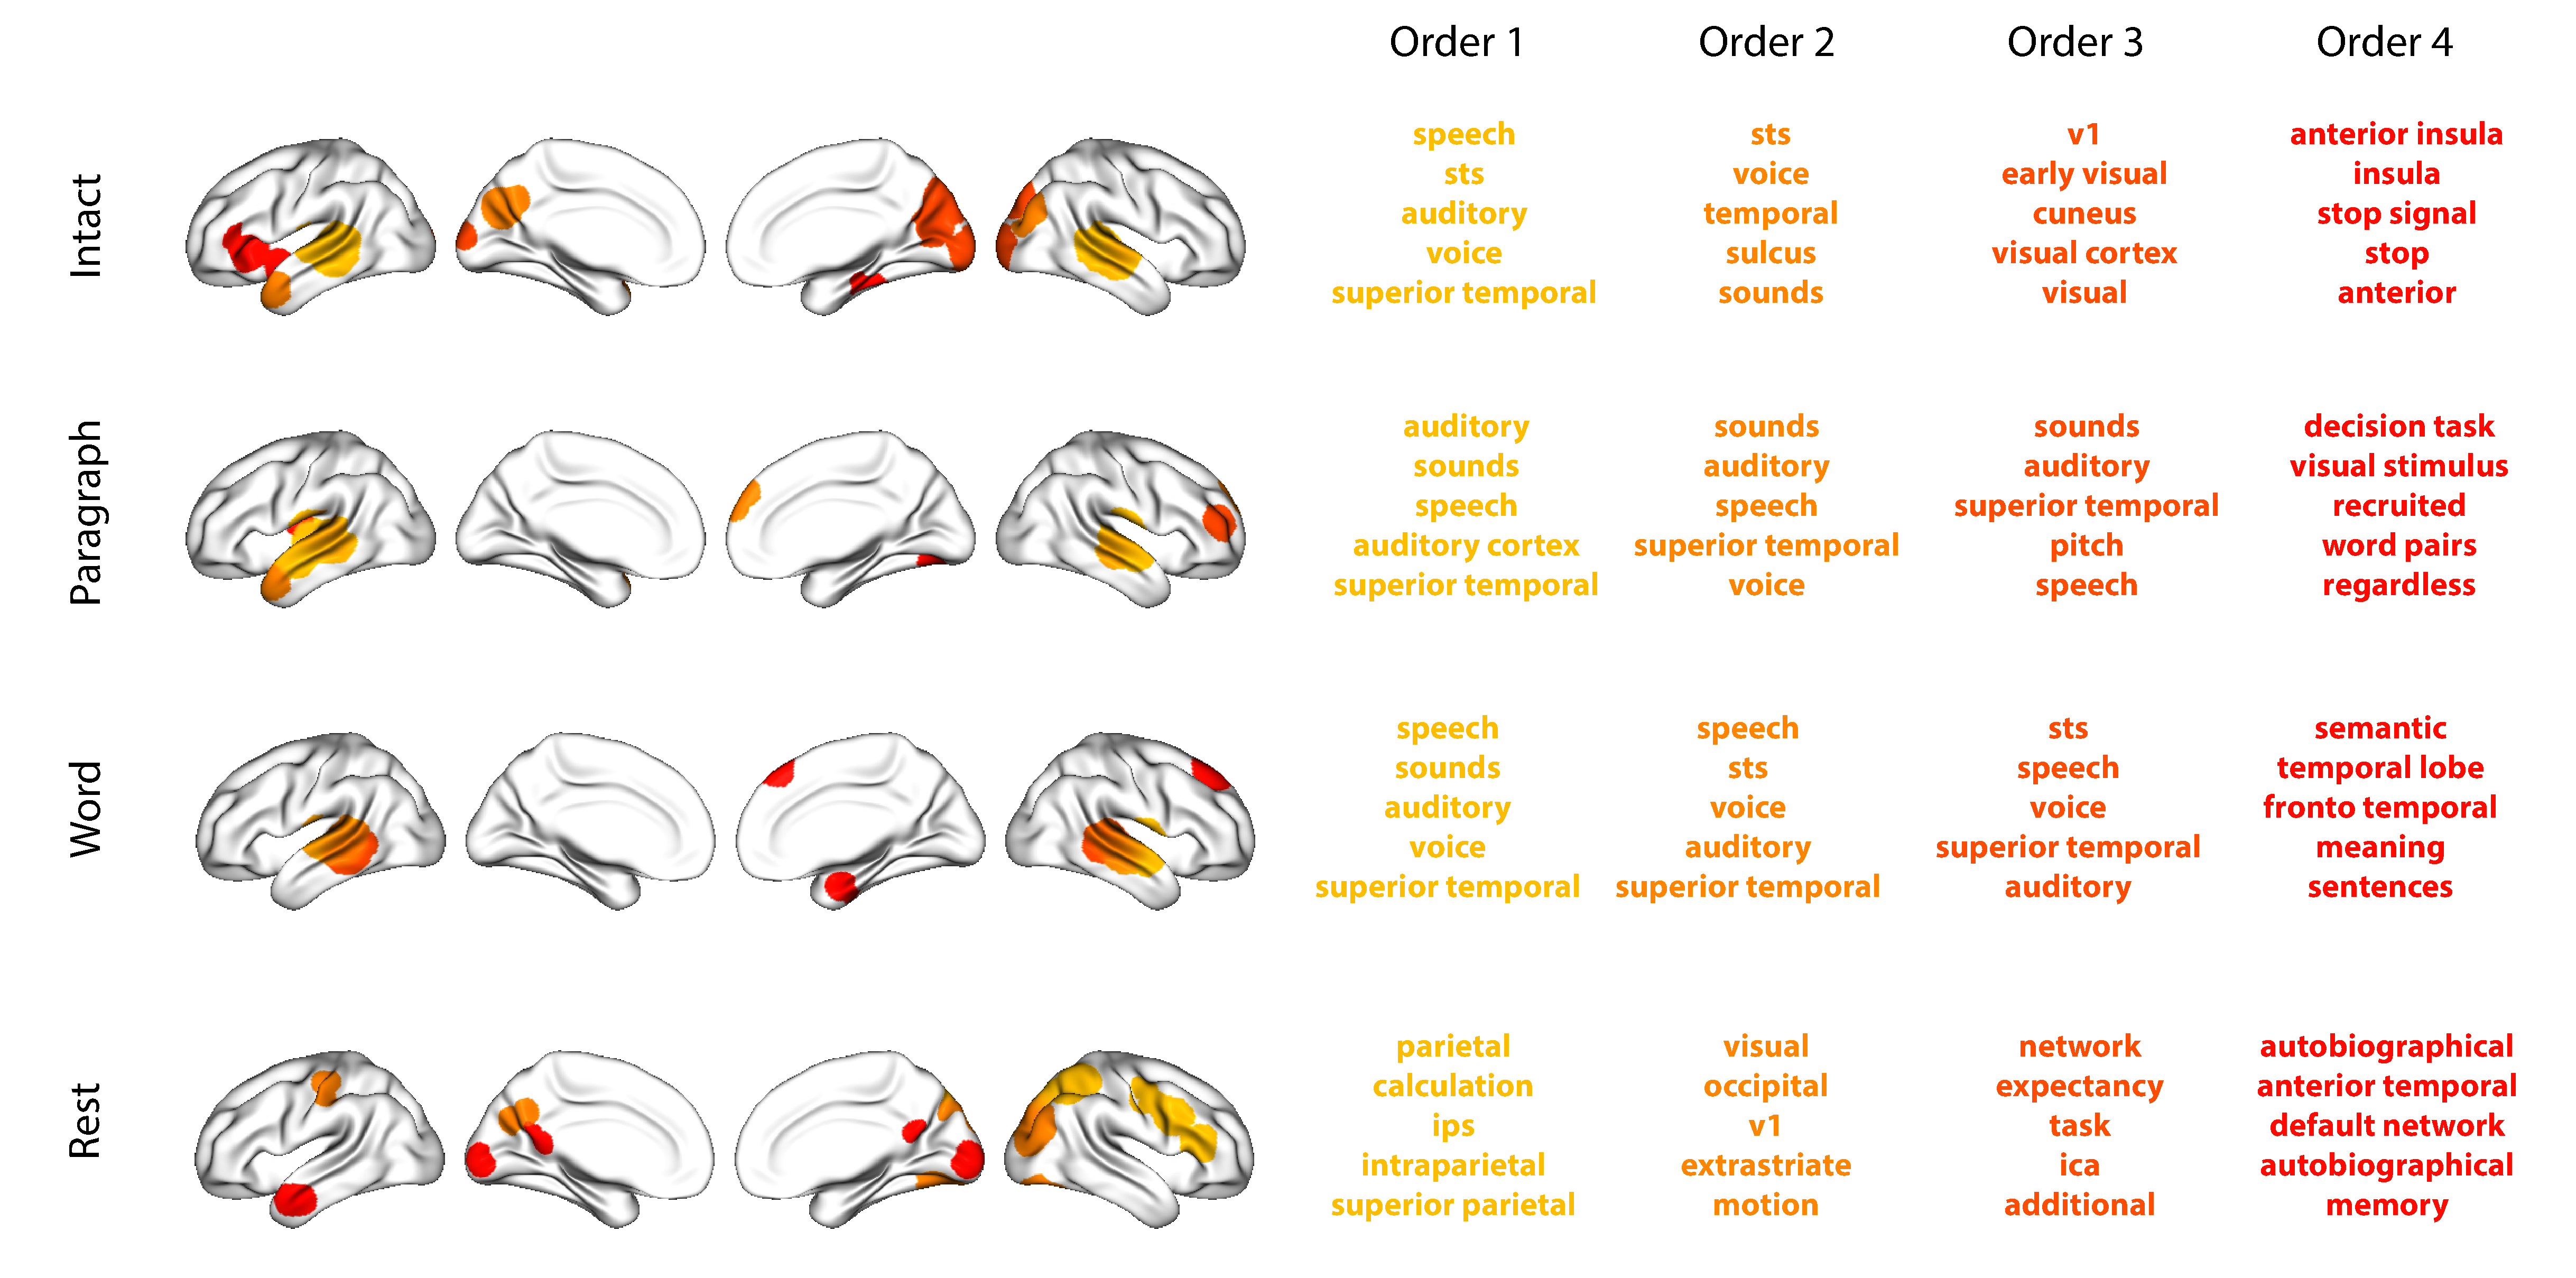
\includegraphics[width=\textwidth]{figs/most_abs}
  \caption{\textbf{Top terms associated with the most strongly
       correlated nodes at each order.}  Each color corresponds to one order of
    inter-subject functional correlations.  To calculate the dynamic
    correlations, eigenvector centrality has been used to project
    the high-dimensional patterns of dynamic correlations onto a
    lower-dimensional space at each previous order, which allows us
    the map the brain regions at each order by retaining the
    features of the original space. The inflated brain plots
    display the locations of the endpoints of the 10 strongest
    (absolute value) correlations at each order, thresholded at 0.999,
    and projected onto the cortical surface~\DIFdelbeginFL \DIFdelFL{\mbox{%DIFAUXCMD
\citep{CombEtal19}}\hspace{0pt}%DIFAUXCMD
}\DIFdelendFL \DIFaddbeginFL \DIFaddFL{\mbox{%DIFAUXCMD
\cite{CombEtal19}}\hspace{0pt}%DIFAUXCMD
}\DIFaddendFL .  The
    lists of terms on the right display the top five Neurosynth
    terms~\DIFdelbeginFL \DIFdelFL{\mbox{%DIFAUXCMD
\citep{RubiEtal17} }\hspace{0pt}%DIFAUXCMD
}\DIFdelendFL \DIFaddbeginFL \DIFaddFL{\mbox{%DIFAUXCMD
\cite{RubiEtal17} }\hspace{0pt}%DIFAUXCMD
}\DIFaddendFL decoded from the corresponding brain maps
    for each order.  Each row displays data from a different
    experimental condition.  Additional maps and their corresponding
    Neurosynth terms may be found in the \DIFdelbeginFL \textit{\DIFdelFL{Supplementary
      materials}} %DIFAUXCMD
\DIFdelendFL \DIFaddbeginFL \DIFaddFL{Supplementary
      materials }\DIFaddendFL (intact: Fig.~\intact; paragraph: Fig.~\para; word:
    Fig.~\word; rest: Fig.~\rest). \DIFaddbeginFL \DIFaddFL{Source data are provided as a Source Data file.}\DIFaddendFL }
  \label{fig:neurosynth}

\end{figure}

Having established that patterns of high-order correlations are
informative to decoders, we next wondered which specific networks of
brain regions contributed most to these patterns.  As a representative
example, we selected the kernel parameters that yielded decoding
accuracies that were the most strongly correlated (across conditions
and orders) with the average accuracies across all of the
kernel parameters we examined.  Using Figure~\ref{fig:decoding}c as a
template, the best-matching kernel was a Laplace kernel with a width
of 50 (Fig.~\ref{fig:kernels}d; also see Fig.~\pca).  We used this kernel to compute a
single $K$ by $K$ $n^\mathrm{th}$-order DISFC matrix for each
experimental condition.  We then used Neurosynth~\DIFdelbegin \DIFdel{\mbox{%DIFAUXCMD
\citep{RubiEtal17} }\hspace{0pt}%DIFAUXCMD
}\DIFdelend \DIFaddbegin \DIFadd{\mbox{%DIFAUXCMD
\cite{RubiEtal17} }\hspace{0pt}%DIFAUXCMD
}\DIFaddend to
compute the terms most highly associated with the most strongly
correlated pairs of regions in each of these matrices
(Fig.~\ref{fig:neurosynth}; see \DIFdelbegin \textit{\DIFdel{Reverse inference}}%DIFAUXCMD
\DIFdelend \DIFaddbegin \DIFadd{Reverse inference}\DIFaddend ).

For all of the story listening conditions (intact, paragraph, and
word; top three rows of Fig.~\ref{fig:neurosynth}), we found that
first- and second-order correlations were most strongly associated
with auditory and speech processing areas.  During intact story
listening, third-order correlations reflected integration with visual
areas, and fourth-order correlations reflected integration with areas
associated with high-level cognition and cognitive control, such as
the ventrolateral prefrontal cortex.  However, when participants
listened to temporally scrambled stories, these higher-order
correlations instead involved interactions with additional regions
associated with speech and semantic processing (second and third rows
of Fig.~\ref{fig:neurosynth}).  By contrast, we found
a much different set of patterns in the resting state data
(Fig.~\ref{fig:neurosynth}, bottom row).
First-order resting state correlations were most strongly associated
with regions involved in counting and numerical understanding.
Second-order resting state correlations were strongest in visual
areas; third-order correlations were strongest in task-positive areas;
and fourth-order correlations were strongest in regions associated
with autobiographical and episodic memory.  We carried out analogous
analyses to create maps (and decode the top associated Neurosynth
terms) for up to fifteenth-order correlations (Figs.~\intact, \para,
\word, and \rest).  Of note, examining fifteenth-order correlations
between 700 nodes using conventional methods would have required
storing roughly
$\frac{700^{2 \times 15}}{2} \approx 1.13 \times 10^{85}$ floating
point numbers-- assuming single-precision (32 bits each), this would
require roughly 32 times as many bits as there are molecules in the
known universe!  Although these fifteenth-order correlations do appear
(visually) to have some well-formed structure, we provide this latter
example primarily as a demonstration of the efficiency and scalability
of our approach.






%%%%%%%%%%%%%%%%%%%%%%%%%%%%%%%%%%%%%%%
\section*{Discussion}
We tested the hypothesis that high-level cognition is reflected in
high-order brain network dynamics~\DIFdelbegin \DIFdel{\mbox{%DIFAUXCMD
\citep[e.g., see][]{SoloEtal19,
  ReimEtal17}}\hspace{0pt}%DIFAUXCMD
}\DIFdelend \DIFaddbegin \DIFadd{\mbox{%DIFAUXCMD
\cite{SoloEtal19,
  ReimEtal17}}\hspace{0pt}%DIFAUXCMD
}\DIFaddend .  We examined high-order network dynamics in functional
neuroimaging data collected during a story listening experiment.  When
participants listened to an auditory recording of the story,
participants exhibited similar high-order brain network dynamics.  By
contrast, when participants instead listened to temporally scrambled
recordings of the story, only lower-order brain network dynamics were
similar across participants.  Our results indicate that higher orders
of network interactions support higher-level aspects of cognitive
processing (Fig.~\ref{fig:discussion}).

\begin{figure}
[tp]
  \centering
  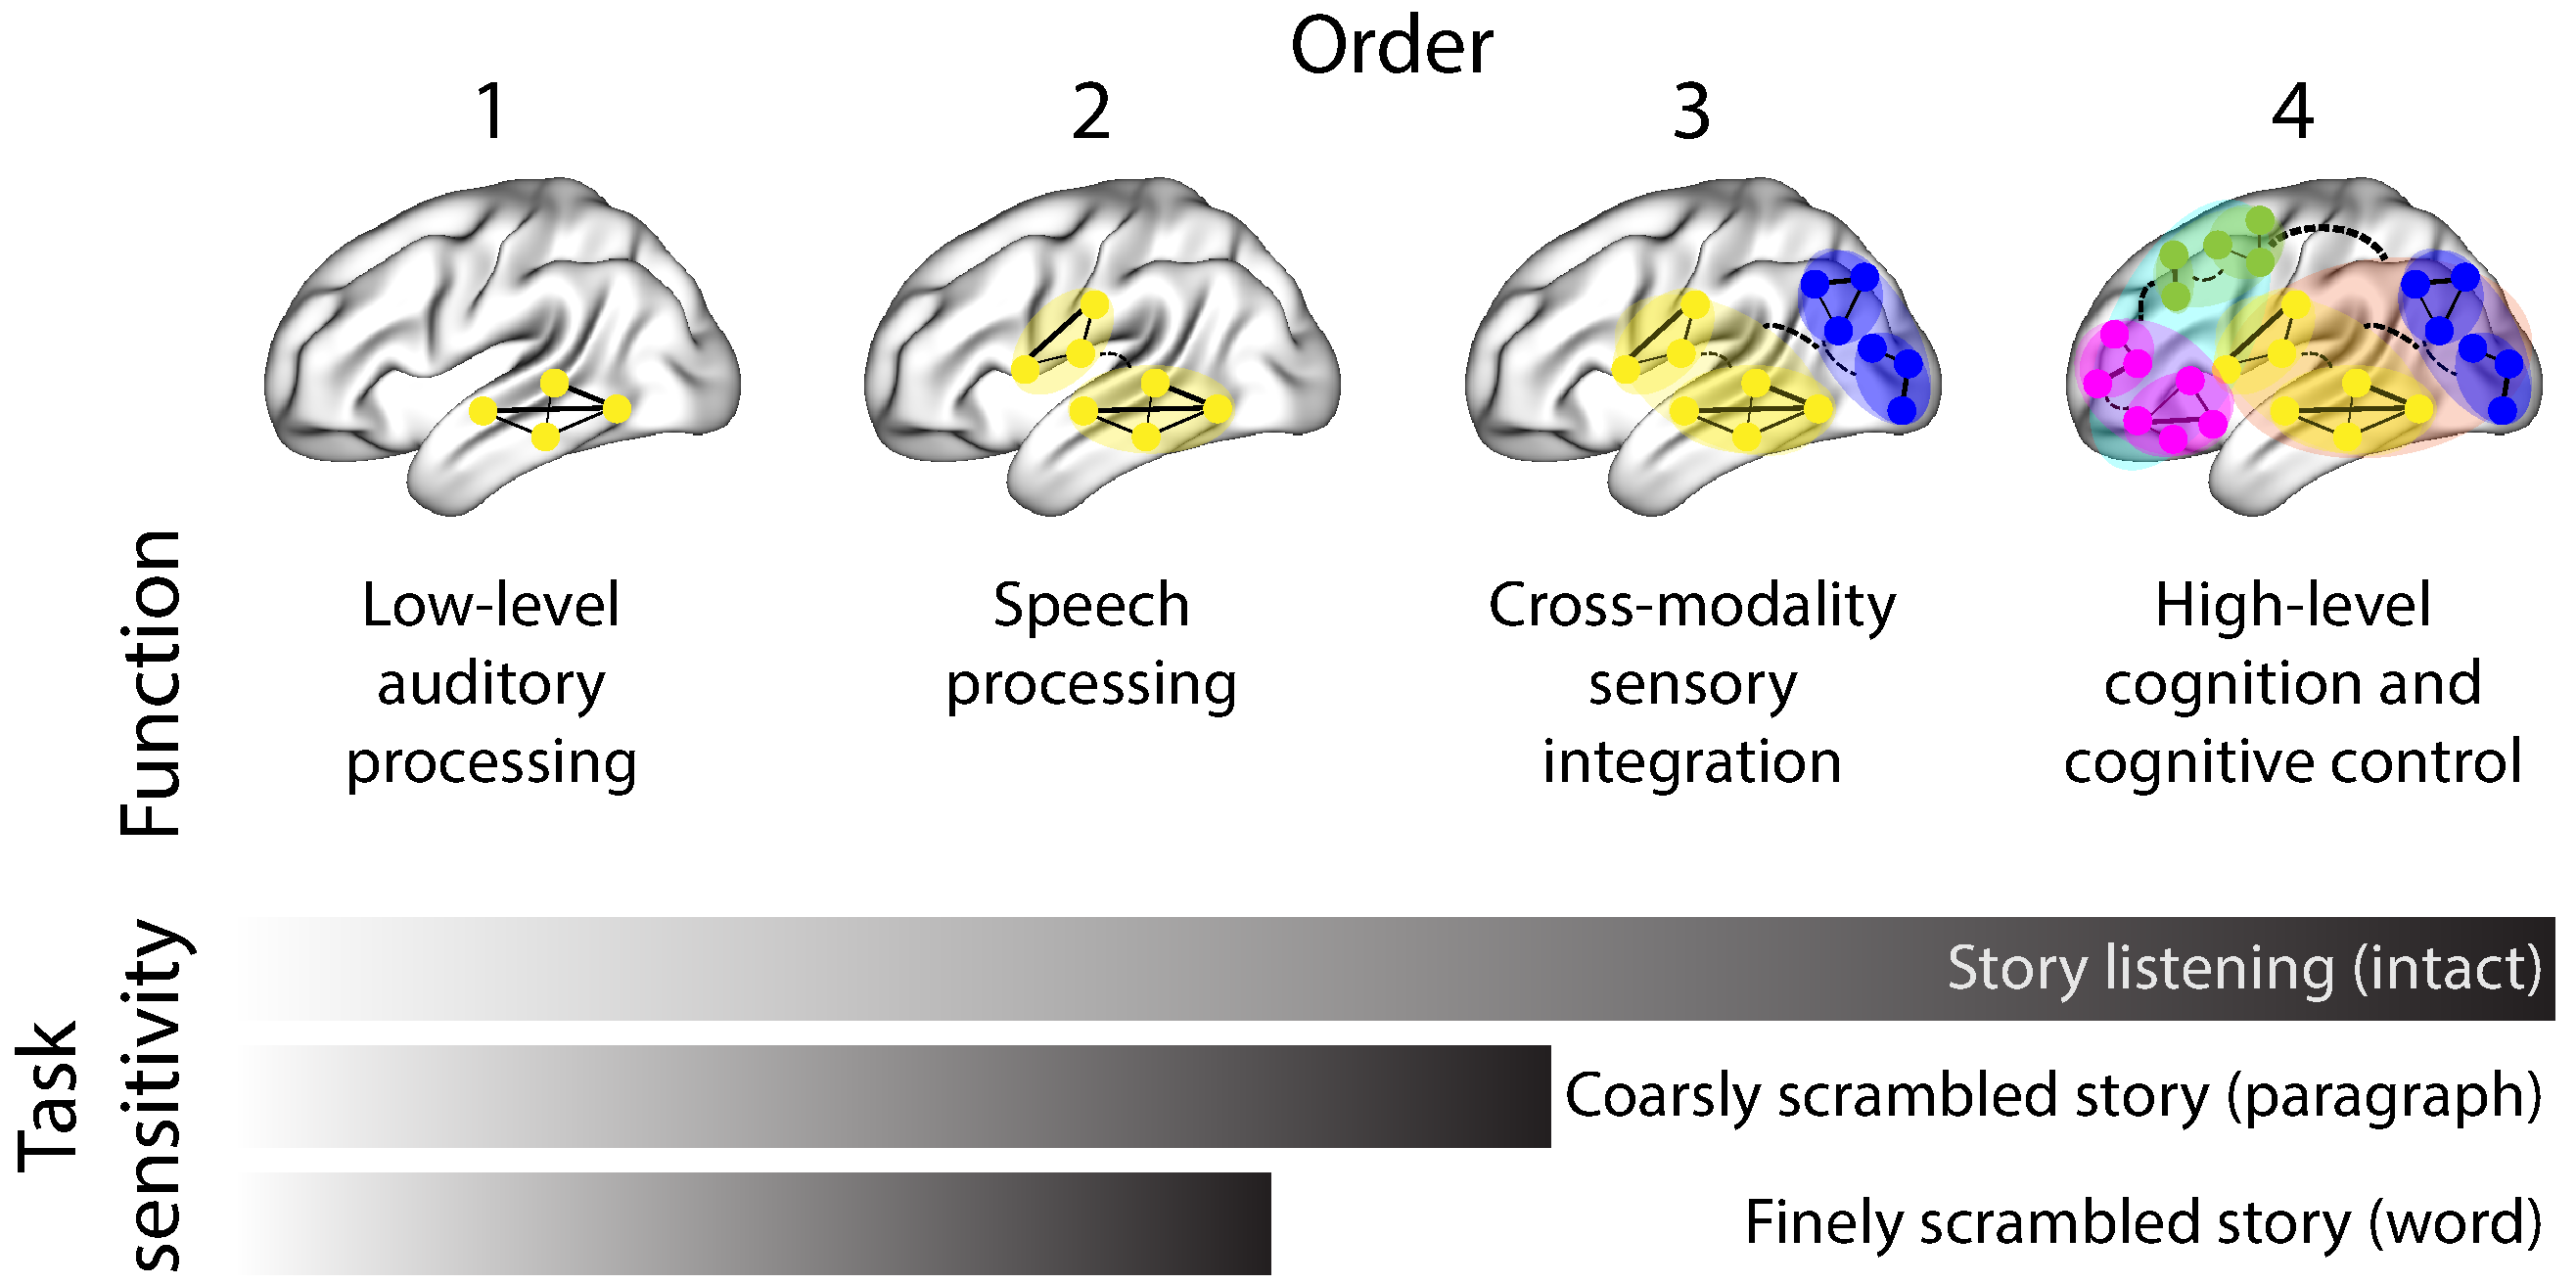
\includegraphics[width=0.6\textwidth]{figs/discussion}
  \caption{\textbf{Proposed high-order network dynamics underlying
       high-level cognition during story listening.}  Schematic depicts
    higher orders of
    network interactions supporting higher-level aspects of cognitive
    processing.  When tasks evoke richer, deeper, and/or higher-level
    processing, this is reflected in higher-order network
    interactions.}
  \label{fig:discussion}

\end{figure}

The notion that cognition is reflected in (and possibly mediated by)
patterns of first-order network dynamics has been suggested by or
proposed in myriad empirical studies and
reviews~\DIFdelbegin \DIFdel{\mbox{%DIFAUXCMD
\citep[e.g.,][]{DemeEtal19, Turk13, LuriEtal18, FongEtal19,
  ParkEtal18b, PretEtal17, MannEtal18, RoyEtal19, LiegEtal19, ZouEtal19,
  ChanGlov10, GonzEtal19, McIn00, BresKels01}}\hspace{0pt}%DIFAUXCMD
}\DIFdelend \DIFaddbegin \DIFadd{\mbox{%DIFAUXCMD
\cite{DemeEtal19, Turk13, LuriEtal18, FongEtal19,
  ParkEtal18b, PretEtal17, MannEtal18, RoyEtal19, LiegEtal19, ZouEtal19,
  ChanGlov10, GonzEtal19, McIn00, BresKels01}}\hspace{0pt}%DIFAUXCMD
}\DIFaddend .  Our study extends this line of work by
finding cognitively relevant \DIFdelbegin \textit{\DIFdel{higher-order}} %DIFAUXCMD
\DIFdelend \DIFaddbegin \DIFadd{higher-order }\DIFaddend network dynamics
that reflect ongoing cognition.  Our findings also complement other work
that uses graph theory and topology to characterize how brain networks
reconfigure during cognition~\DIFdelbegin \DIFdel{\mbox{%DIFAUXCMD
\citep[e.g.,][]{BassEtal06, ZhenEtal19,
  McInJirs19, TokeSomm19, SizeEtal18, ReimEtal17, BetzEtal19}}\hspace{0pt}%DIFAUXCMD
}\DIFdelend \DIFaddbegin \DIFadd{\mbox{%DIFAUXCMD
\cite{BassEtal06, ZhenEtal19,
  McInJirs19, TokeSomm19, SizeEtal18, ReimEtal17, BetzEtal19}}\hspace{0pt}%DIFAUXCMD
}\DIFaddend .

An open question not addressed by our study pertains to how different
structures integrate incoming information with different time
constants.  For example, one line of work suggests that the cortical
surface comprises a structured map such that nearby brain structures
process incoming information at similar timescales.  Low-level sensory
areas integrate information relatively quickly, whereas higher-level
regions integrate information relatively slowly~\DIFdelbegin \DIFdel{\mbox{%DIFAUXCMD
\citep{BaldEtal17,
  HassEtal08, HassEtal15, HoneEtal12a, LernEtal11, LernEtal14,
  ChieHone19}}\hspace{0pt}%DIFAUXCMD
}\DIFdelend \DIFaddbegin \DIFadd{\mbox{%DIFAUXCMD
\cite{BaldEtal17,
  HassEtal08, HassEtal15, HoneEtal12a, LernEtal11, LernEtal14,
  ChieHone19}}\hspace{0pt}%DIFAUXCMD
}\DIFaddend .  A similar hierarchy appears to play a role in
predicting future events~\DIFdelbegin \DIFdel{\mbox{%DIFAUXCMD
\citep{LeeEtal20}}\hspace{0pt}%DIFAUXCMD
}\DIFdelend \DIFaddbegin \DIFadd{\mbox{%DIFAUXCMD
\cite{LeeEtal20}}\hspace{0pt}%DIFAUXCMD
}\DIFaddend .  Other related work in
human and mouse brains indicates that the temporal response profile of
a given brain structure may relate to how strongly connected that
structure is with other brain areas~\DIFdelbegin \DIFdel{\mbox{%DIFAUXCMD
\citep{FallEtal20}}\hspace{0pt}%DIFAUXCMD
}\DIFdelend \DIFaddbegin \DIFadd{\mbox{%DIFAUXCMD
\cite{FallEtal20}}\hspace{0pt}%DIFAUXCMD
}\DIFaddend .  Further study
is needed to understand the role of temporal integration at different
scales of network interaction, and across different anatomical
structures. Importantly, our analyses do not speak to the
physiological basis of higher-order dynamics, and could reflect
nonlinearities, chaotic patterns, non-stationarities, and/or
multistability, etc. However, our decoding analyses do indicate that
higher-order dynamics are consistent across individuals, and therefore
unlikely to reflect non-stimulus-driven dynamics that are unlikely to
be similar across individuals.

One limitation of our approach relates to how noise propagates in our
estimation procedure.  Specifically, our procedure for estimating
high-order dynamic correlations depends on estimates of lower-order
dynamic correlations.  This means that our measures of which
higher-order patterns are reliable and stable across experimental
conditions are partially confounded with the stability of lower-order
patterns.  Prior work suggests that the stability of what we refer to
here as first-order dynamics likely varies across the experimental
conditions we examined~\DIFdelbegin \DIFdel{\mbox{%DIFAUXCMD
\citep{SimoEtal16}}\hspace{0pt}%DIFAUXCMD
}\DIFdelend \DIFaddbegin \DIFadd{\mbox{%DIFAUXCMD
\cite{SimoEtal16}}\hspace{0pt}%DIFAUXCMD
}\DIFaddend .  Therefore a caveat to our
claim that richer stimuli evoke more stable higher-order dynamics is
that our approach assumes that those high-order dynamics reflect
relations or interactions between lower-order features.

Another potential limitation of our approach relates to recent work
suggesting that the brain undergoes rapid state changes, for example
across event boundaries~\DIFdelbegin \DIFdel{\mbox{%DIFAUXCMD
\citep[e.g.,][]{BaldEtal17}}\hspace{0pt}%DIFAUXCMD
}\DIFdelend \DIFaddbegin \DIFadd{\mbox{%DIFAUXCMD
\cite{BaldEtal17}}\hspace{0pt}%DIFAUXCMD
}\DIFaddend .
\cite{ShapEtal19} used hidden semi-Markov models to estimate
state-specific network dynamics~\DIFdelbegin \DIFdel{\mbox{%DIFAUXCMD
\citep[also see][]{VidaEtal18}}\hspace{0pt}%DIFAUXCMD
}\DIFdelend \DIFaddbegin \DIFadd{\mbox{%DIFAUXCMD
\cite{VidaEtal18}}\hspace{0pt}%DIFAUXCMD
}\DIFaddend .  Our
general approach might be extended by considering putative state
transitions. For example, rather than weighting all timepoints using a
similar kernel (Eqn.~\ref{eqn:timecorr}), the kernel function could
adapt on a timepoint-by-timepoint basis such that only timepoints
determined to be in the same ``state'' were given non-zero weight.

Identifying high-order network dynamics associated with high-level
cognition required several important methods advances.  First, we used
kernel-based dynamic correlations to extended the notion of (static)
inter-subject functional connectivity~\DIFdelbegin \DIFdel{\mbox{%DIFAUXCMD
\citep{SimoEtal16} }\hspace{0pt}%DIFAUXCMD
}\DIFdelend \DIFaddbegin \DIFadd{\mbox{%DIFAUXCMD
\cite{SimoEtal16} }\hspace{0pt}%DIFAUXCMD
}\DIFaddend to a dynamic
measure of inter-subject functional connectivity (DISFC) that does not
rely on sliding windows~\DIFdelbegin \DIFdel{\mbox{%DIFAUXCMD
\citep[e.g., as in][]{MannEtal18}}\hspace{0pt}%DIFAUXCMD
}\DIFdelend \DIFaddbegin \DIFadd{\mbox{%DIFAUXCMD
\cite{MannEtal18}}\hspace{0pt}%DIFAUXCMD
}\DIFaddend , and that
may be computed at individual timepoints.  This allowed us to
precisely characterize stimulus-evoked network dynamics that were
similar across individuals.  Second, we developed a computational
framework for efficiently and scalably estimating high-order dynamic
correlations.  Our approach uses dimensionality reduction algorithms
and graph measures to obtain low-dimensional embeddings of patterns of
network dynamics.  Third, we developed an analysis framework for
identifying robust decoding results by carrying out our analyses using
a range of parameter values and identifying which results were robust
to specific parameter choices. By showing that high-level cognition is
reflected in high-order network dynamics, we have elucidated the next
step on the path towards understanding the neural basis of cognition.



\section*{Methods}
Our general approach to efficiently estimating high-order dynamic
correlations comprises four general steps (Fig.~\ref{fig:methods}).
First, we derive a kernel-based approach to computing dynamic pairwise
correlations in a $T$ (timepoints) by $K$ (features) multivariate
timeseries, $\mathbf{X}_0$.  This yields a $T$ by $\mathcal{O}(K^2)$
matrix of dynamic correlations, $\mathbf{Y}_1$, where each row
comprises the upper triangle and diagonal of the correlation matrix at a single
timepoint, reshaped into a row vector (this reshaped vector is
$\left( \frac{K^2 - K}{2} + K \right)$-dimensional).  Second, we apply a dimensionality
reduction step to project the matrix of dynamic correlations back onto
a $K$-dimensional space.  This yields a $T$ by $K$ matrix,
$\mathbf{X}_1$, that reflects an approximation of the dynamic
correlations reflected in the original data.  Third, we use repeated
applications of the kernel-based dynamic correlation step to
$\mathbf{X}_n$ and the dimensionality reduction step to the resulting
$\mathbf{Y}_{n+1}$ to estimate high-order dynamic correlations.  Each
application of these steps to a $T$ by $K$ time series $\mathbf{X}_n$
yields a $T$ by $K$ matrix, $\mathbf{X}_{n+1}$, that reflects the
dynamic correlations between the columns of $\mathbf{X}_n$.  In this
way, we refer to $n$ as the \DIFdelbegin \textit{\DIFdel{order}} %DIFAUXCMD
\DIFdelend \DIFaddbegin \DIFadd{order }\DIFaddend of the timeseries, where
$\mathbf{X}_0$ (order 0) denotes the original data and $\mathbf{X}_n$
denotes (approximated) $n^\mathrm{th}$-order dynamic correlations
between the columns of $\mathbf{X}_0$.  Finally, we use a
cross-validation--based decoding approach to evaluate how well
information contained in a given order (or weighted mixture of orders)
may be used to decode relevant cognitive states.  If including a given
$\mathbf{X}_n$ in the feature set yields higher classification
accuracy on held-out data, we interpret this as evidence that the
given cognitive states are reflected in patterns of
$n^\mathrm{th}$-order correlations.

All of the code used to produce
the figures and results in this manuscript, along with links to the
corresponding datasets, may be found at
\href{https://github.com/ContextLab/timecorr-paper}{github.com/ContextLab/timecorr-paper}.
In addition, we have released a Python toolbox for computing dynamic
high-order correlations in timeseries data; our toolbox may be found
at
\href{https://timecorr.readthedocs.io/}{timecorr.readthedocs.io}.
\begin{figure}
  \centering
  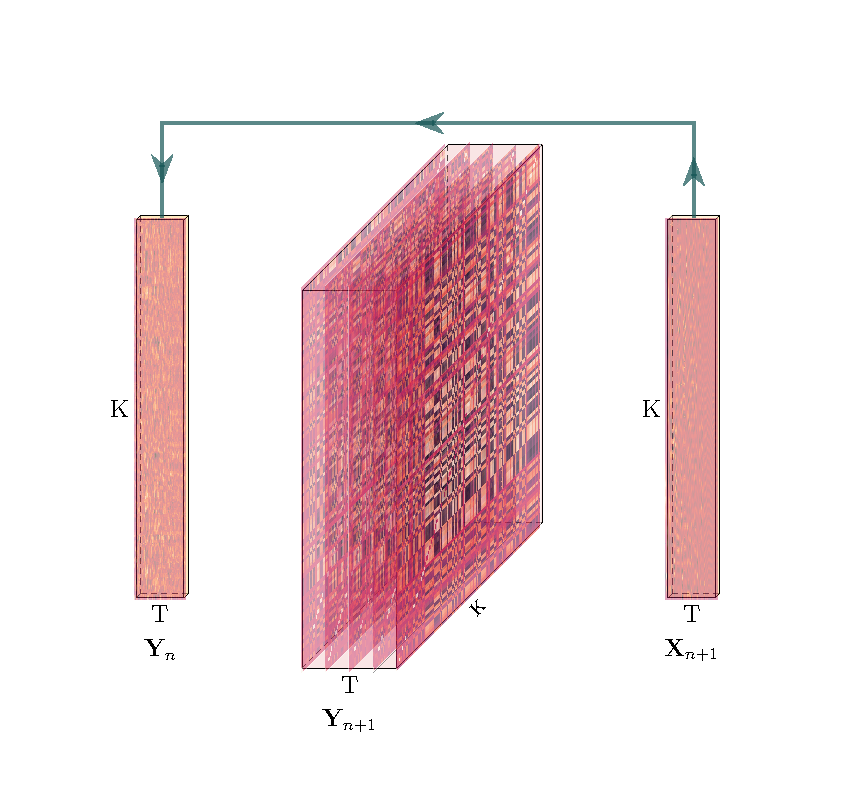
\includegraphics[width=0.5\textwidth]{figs/methods_fig}
  \caption{\textbf{Estimating dynamic high-order correlations.}  Given
    a $T$ by $K$ matrix of multivariate timeseries data,
    $\mathbf{X}_n$ (where $n \in \mathbb{N}, n \geq 0$), we use
    Equation~\ref{eqn:timecorr} to compute a timeseries of
    $K$ by $K$ correlation matrices, $\mathbf{Y}_{n+1}$.  We then
    approximate $\mathbf{Y}_{n+1}$ with the $T$ by $K$ matrix
    $\mathbf{X}_{n+1}$.  This process may be repeated to scalably estimate
    iteratively higher-order correlations in the data.  Note that the
    transposes of $\mathbf{X}_n$ and $\mathbf{X}_{n+1}$ are displayed
    in the figure for compactness.
  \label{fig:methods}}

\end{figure}


\subsection*{Kernel-based approach for computing dynamic correlations}
Given a $T$ by $K$ matrix of observations, $\mathbf{X}$, we can compute the (static)
Pearson's correlation between any pair of columns, $\mathbf{X}(\cdot, i)$ and
$\mathbf{X}(\cdot, j)$ using~\DIFdelbegin \DIFdel{\mbox{%DIFAUXCMD
\citep{Pear01}}\hspace{0pt}%DIFAUXCMD
}\DIFdelend \DIFaddbegin \DIFadd{\mbox{%DIFAUXCMD
\cite{Pear01}}\hspace{0pt}%DIFAUXCMD
}\DIFaddend :
\begin{align}
  \mathrm{corr}(\mathbf{X}(\cdot, i), \mathbf{X}(\cdot, j)) &=
                                                              \frac{\sum_{t=1}^T
                                                              \left(\mathbf{X}(t,
                                                              i)
                                                              -
                                                              \bar{\mathbf{X}}(\cdot,
                                                              i)\right)
                                                              \left(\mathbf{X}(t,
                                                              j)
                                                              -
                                                              \bar{\mathbf{X}}(\cdot, j)\right)}{\sqrt{\sum_{t=1}^T
                                                              \sigma^2_{\mathbf{X}(\cdot, i)} 
                                                              \sigma^2_{\mathbf{X}(\cdot, j)}}},~\mathrm{where}\label{eqn:corr}\\
  \bar{\mathbf{X}}(\cdot, k) &= \frac{1}{T}\sum_{t=1}^T
                               \mathbf{X}(t, k),~\mathrm{and}\\
  \sigma^2_{\mathbf{X}(\cdot, k)} &= \frac{1}{T}\sum_{t=1}^T \left( \mathbf{X}(t, k) -
                                    \bar{\mathbf{X}}(\cdot, k) \right)^2 
\end{align}
We can generalize this formula to compute time-varying correlations by
incorporating a \DIFdelbegin \textit{\DIFdel{kernel function}} %DIFAUXCMD
\DIFdelend \DIFaddbegin \DIFadd{kernel function }\DIFaddend that takes a time $t$ as
input, and returns how much the observed data at each timepoint
$\tau \in \left[ -\infty, \infty \right]$ contributes to the estimated instantaneous
correlation\DIFaddbegin \DIFadd{~\mbox{%DIFAUXCMD
\cite{AlleEtal12b} }\hspace{0pt}%DIFAUXCMD
}\DIFaddend at time $t$ \DIFdelbegin \DIFdel{~\mbox{%DIFAUXCMD
\citep[Fig.~\ref{fig:kernels}; also see][for a
similar approach]{AlleEtal12b}}\hspace{0pt}%DIFAUXCMD
}\DIFdelend \DIFaddbegin \DIFadd{(Fig.~\ref{fig:kernels})}\DIFaddend .

\begin{figure}
  \centering
  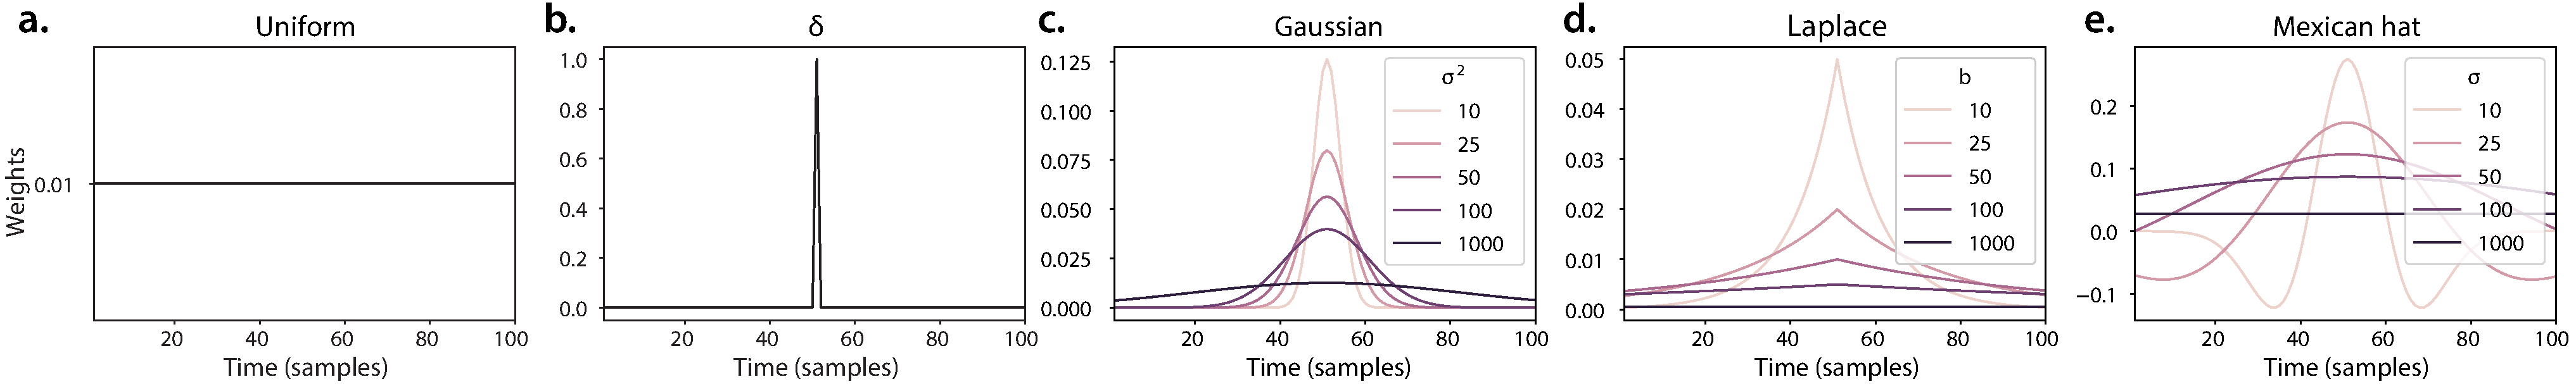
\includegraphics[width=\textwidth]{figs/kernels}
  \caption{\textbf{Examples of kernel functions.} Each panel displays
    per-timepoint weights for a kernel centered at $t = 50$, evaluated
    at 100 timepoints ($\tau \in \left[1, ..., 100\right]$).
   \textbf{a. Uniform kernel.} The weights are timepoint-invariant;
    observations at all timepoints are weighted equally, and do not
    change as a function of $\tau$.  This is a special case kernel
    function that reduces dynamic correlations to static correlations.
   \textbf{b. Dirac $\delta$ kernel.} Only the observation at
    timepoint $t$ is given a non-zero weight (of 1).
   \textbf{c. Gaussian kernels.} Each kernel's weights fall off in
    time according to a Gaussian probability density function centered
    on time $t$.  Weights derived using several different example
    width parameters ($\sigma^2$) are displayed.  \textbf{d. Laplace
       kernels.}  Each kernel's weights fall off in time according to a
    Laplace probability density function centered on time $t$.
    Weights derived using several different example width parameters
    ($b$) are displayed.  \textbf{e. Mexican hat (Ricker wavelet)
       kernels.}  Each kernel's weights fall off in time according to a
    Ricker wavelet centered on time $t$.  This function highlights the
    \DIFdelbeginFL \textit{\DIFdelFL{contrasts}} %DIFAUXCMD
\DIFdelendFL \DIFaddbeginFL \DIFaddFL{contrasts }\DIFaddendFL between local versus surrounding activity
    patterns in estimating dynamic correlations. Weights derived using
    several different example width parameters ($\sigma$) are
    displayed.}
  \label{fig:kernels}

\end{figure}

Given a kernel function $\kappa_t(\cdot)$ for timepoint $t$,
evaluated at timepoints $\tau \in \left[ 1, ..., T \right]$, we
can update the static correlation formula in Equation~\ref{eqn:corr}
to estimate the \DIFdelbegin \textit{\DIFdel{instantaneous correlation}} %DIFAUXCMD
\DIFdelend \DIFaddbegin \DIFadd{instantaneous correlation }\DIFaddend at timepoint $t$:
\begin{align}
  \mathrm{timecorr}_{\kappa_t}\left(\mathbf{X}(\cdot, i), \mathbf{X}(\cdot, j)\right) &= \frac{\sum_{\tau=1}^T \left( \mathbf{X}(\tau, i) -
                                       \widetilde{\mathbf{X}}_{\kappa_t}(\cdot,
                                                                                        i) \right)
                                 \left( \mathbf{X}(\tau, j) -
                                        \widetilde{\mathbf{X}}_{\kappa_t}(\cdot,
                                                                                        j)\right)}{\sqrt{\sum_{\tau=1}^T
                                              \widetilde{\sigma}_{\kappa_t}^2(\mathbf{X}(\cdot,
                                                                                        i))
                                              \widetilde{\sigma}_{\kappa_t}^2(\mathbf{X}(\cdot, j))}},~\mathrm{where}\label{eqn:timecorr}\\
  \widetilde{\mathbf{X}}_{\kappa_t}(\cdot, k) &= \sum_{\tau=1}^T
                       \kappa_t(\tau)\mathbf{X}(\tau, k),\\
  \widetilde{\sigma}_{\kappa_t}^2(\mathbf{X}(\cdot, k)) &= \sum_{\tau=1}^T
                                                  \left(
                                                  \mathbf{X}(\tau, k) -
                            \widetilde{\mathbf{X}}_{\kappa_t}(\cdot, k) \right)^2.
\end{align}
Here
$\mathrm{timecorr}_{\kappa_t}(\mathbf{X}(\cdot, i), \mathbf{X}(\cdot,
j))$ reflects the correlation at time $t$ between columns $i$ and $j$
of $\mathbf{X}$, estimated using the kernel $\kappa_t$.  We evaluate
Equation~\ref{eqn:timecorr} in turn for each pair of columns in
$\mathbf{X}$ and for kernels centered on each timepoint in the
timeseries, respectively, to obtain a $T$ by $K$ by $K$ timeseries of
dynamic correlations, $\mathbf{Y}$.  For convenience, we then reshape
the upper triangles and diagonals of each timepoint's symmetric correlation matrix into a row
vector to obtain an equivalent $T$ by $\left( \frac{K^2 - K}{2} + K \right)$ matrix.

\subsubsection*{Dynamic inter-subject functional connectivity (DISFC)}
Equation~\ref{eqn:timecorr} provides a means of taking a single
observation matrix, $\mathbf{X}_n$ and estimating the dynamic
correlations from moment to moment, $\mathbf{Y}_{n+1}$.  Suppose that
one has access to a set of multiple observation matrices that reflect
the same phenomenon.  For example, one might collect neuroimaging data
from several experimental participants, as each participant performs
the same task (or sequence of tasks).  Let $\mathbf{X}_n^1$,
$\mathbf{X}_n^2$, ..., $\mathbf{X}_n^P$ reflect the $T$ by $K$
observation matrices ($n = 0$) or reduced correlation matrices
($n > 0$) for each of $P$ participants in an experiment.  We can use
\DIFdelbegin \textit{\DIFdel{inter-subject functional connectivity}}%DIFAUXCMD
\DIFdel{~\mbox{%DIFAUXCMD
\citep[ISFC;
][]{SimoEtal16, SimoChan20} }\hspace{0pt}%DIFAUXCMD
}\DIFdelend \DIFaddbegin \DIFadd{inter-subject functional connectivity~\mbox{%DIFAUXCMD
\cite{SimoEtal16, SimoChan20}
}\hspace{0pt}%DIFAUXCMD
(ISFC) }\DIFaddend to compute the stimulus-driven correlations reflected
in the multi-participant dataset at a given timepoint $t$ using:
\begin{align}
\bar{\mathbf{C}}(t) = M\left(R\left(\frac{1}{2P} \sum_{p=1}^P
  Z\left(\mathbf{Y}_{n+1}^p(t)\right)^\top + Z\left(\mathbf{Y}_{n+1}^p(t)\right)\right)\right),\label{eqn:disfc}
\end{align}
where $M$ extracts and vectorizes the upper triangle and diagonal of a symmetric
matrix, $Z$ is the Fisher $z$-transformation~\DIFdelbegin \DIFdel{\mbox{%DIFAUXCMD
\citep{Zar10}}\hspace{0pt}%DIFAUXCMD
}\DIFdelend \DIFaddbegin \DIFadd{\mbox{%DIFAUXCMD
\cite{Zar10}}\hspace{0pt}%DIFAUXCMD
}\DIFaddend :
\begin{align}
Z(r) = \frac{\log(1+r) - \log(1-r)}{2},
\end{align}
$R$ is the inverse of $Z$:
\begin{align}
R(z) = \frac{\exp(2z - 1)}{\exp(2z + 1)},
\end{align}
and $\mathbf{Y}_{n+1}^p(t)$ denotes the correlation matrix at timepoint $t$
(Eqn.~\ref{eqn:timecorr}) between each column of $\mathbf{X}_n^p$ and each
column of the average $\mathbf{X}_n$ from all \DIFdelbegin \textit{\DIFdel{other}}
%DIFAUXCMD
\DIFdelend \DIFaddbegin \DIFadd{other
}\DIFaddend participants, $\bar{\mathbf{X}}_n^{ \backslash p}$:
\begin{align}
  \bar{\mathbf{X}}_n^{ \backslash p} = \frac{1}{P-1}\sum_{q \in
  \backslash p} \mathbf{X}_n^q,
\end{align}
where $\backslash p$ denotes the set of all participants other than
participant $p$. In this way, the $T$ by $\left( \frac{K^2 - K}{2} + K \right)$ DISFC
matrix $\bar{\mathbf{C}}$ provides a time-varying extension of the ISFC
approach developed by \cite{SimoEtal16}.

\subsection*{Low-dimensional representations of dynamic
  correlations}

Given a $T$ by $\left( \frac{K^2 - K}{2} + K \right)$ matrix of
$n^\mathrm{th}$-order dynamic correlations, $\mathbf{Y}_n$, we propose
two general approaches to computing a $T$ by $K$ low-dimensional
representation of those correlations, $\mathbf{X}_n$.  The first
approach uses dimensionality reduction algorithms to project
$\mathbf{Y}_n$ onto a $K$-dimensional space.  The second approach uses
graph measures to characterize the relative positions of each feature
($k \in \left[1, ..., K \right]$) in the network defined by the
correlation matrix at each timepoint.

\subsubsection*{Dimensionality reduction-based approaches to computing
  $\mathbf{X}_n$}

The modern toolkit of dimensionality reduction algorithms include
Principal Components Analysis~\DIFdelbegin \DIFdel{\mbox{%DIFAUXCMD
\citep[PCA;][]{Pear01}}\hspace{0pt}%DIFAUXCMD
}\DIFdelend \DIFaddbegin \DIFadd{\mbox{%DIFAUXCMD
\cite{Pear01} }\hspace{0pt}%DIFAUXCMD
(PCA)}\DIFaddend , Probabilistic
PCA~\DIFdelbegin \DIFdel{\mbox{%DIFAUXCMD
\citep[PPCA;][]{TippBish99}}\hspace{0pt}%DIFAUXCMD
}\DIFdelend \DIFaddbegin \DIFadd{\mbox{%DIFAUXCMD
\cite{TippBish99} }\hspace{0pt}%DIFAUXCMD
(PPCA)}\DIFaddend , Exploratory Factor
Analysis~\DIFdelbegin \DIFdel{\mbox{%DIFAUXCMD
\citep[EFA;][]{Spea04}}\hspace{0pt}%DIFAUXCMD
}\DIFdelend \DIFaddbegin \DIFadd{\mbox{%DIFAUXCMD
\cite{Spea04} }\hspace{0pt}%DIFAUXCMD
(EFA)}\DIFaddend , Independent Components
Analysis~\DIFdelbegin \DIFdel{\mbox{%DIFAUXCMD
\citep[ICA;][]{JuttHera91, ComoEtal91}}\hspace{0pt}%DIFAUXCMD
}\DIFdelend \DIFaddbegin \DIFadd{\mbox{%DIFAUXCMD
\cite{JuttHera91, ComoEtal91} }\hspace{0pt}%DIFAUXCMD
(ICA)}\DIFaddend , $t$-Stochastic
Neighbor Embedding~\DIFdelbegin \DIFdel{\mbox{%DIFAUXCMD
\citep[$t$-SNE;][]{vandHint08}}\hspace{0pt}%DIFAUXCMD
}\DIFdelend \DIFaddbegin \DIFadd{\mbox{%DIFAUXCMD
\cite{vandHint08} }\hspace{0pt}%DIFAUXCMD
($t$-SNE)}\DIFaddend , Uniform Manifold
Approximation and Projection~\DIFdelbegin \DIFdel{\mbox{%DIFAUXCMD
\citep[UMAP;][]{McInEtal18}}\hspace{0pt}%DIFAUXCMD
}\DIFdelend \DIFaddbegin \DIFadd{\mbox{%DIFAUXCMD
\cite{McInEtal18} }\hspace{0pt}%DIFAUXCMD
(UMAP)}\DIFaddend , non-negative
matrix factorization~\DIFdelbegin \DIFdel{\mbox{%DIFAUXCMD
\citep[NMF;][]{LeeSeun99}}\hspace{0pt}%DIFAUXCMD
}\DIFdelend \DIFaddbegin \DIFadd{\mbox{%DIFAUXCMD
\cite{LeeSeun99} }\hspace{0pt}%DIFAUXCMD
(NMF)}\DIFaddend , Topographic Factor
Analysis~\DIFdelbegin \DIFdel{\mbox{%DIFAUXCMD
\cite[TFA;][]{MannEtal14b}}\hspace{0pt}%DIFAUXCMD
}\DIFdelend \DIFaddbegin \DIFadd{\mbox{%DIFAUXCMD
\cite{MannEtal14b} }\hspace{0pt}%DIFAUXCMD
(TFA)}\DIFaddend , Hierarchical Topographic Factor
analysis~\DIFdelbegin \DIFdel{\mbox{%DIFAUXCMD
\cite[HTFA;][]{MannEtal18}}\hspace{0pt}%DIFAUXCMD
}\DIFdelend \DIFaddbegin \DIFadd{\mbox{%DIFAUXCMD
\cite{MannEtal18} }\hspace{0pt}%DIFAUXCMD
(HTFA)}\DIFaddend , Topographic Latent Source
Analysis~\DIFdelbegin \DIFdel{\mbox{%DIFAUXCMD
\cite[TLSA;][]{GersEtal11}}\hspace{0pt}%DIFAUXCMD
}\DIFdelend \DIFaddbegin \DIFadd{\mbox{%DIFAUXCMD
\cite{GersEtal11} }\hspace{0pt}%DIFAUXCMD
(TLSA)}\DIFaddend , dictionary
learning~\DIFdelbegin \DIFdel{\mbox{%DIFAUXCMD
\citep{MairEtal09a, MairEtal09b}}\hspace{0pt}%DIFAUXCMD
}\DIFdelend \DIFaddbegin \DIFadd{\mbox{%DIFAUXCMD
\cite{MairEtal09a, MairEtal09b}}\hspace{0pt}%DIFAUXCMD
}\DIFaddend , and deep
auto-encoders~\DIFdelbegin \DIFdel{\mbox{%DIFAUXCMD
\citep{HintSala06}}\hspace{0pt}%DIFAUXCMD
}\DIFdelend \DIFaddbegin \DIFadd{\mbox{%DIFAUXCMD
\cite{HintSala06}}\hspace{0pt}%DIFAUXCMD
}\DIFaddend , among others.  While complete
characterizations of each of these algorithms is beyond the scope of
the present manuscript, the general intuition driving these approaches
is to compute the $T$ by $K$ matrix, $\mathbf{X}$, that is closest to
the original $T$ by $J$ matrix, $\mathbf{Y}$, where (typically)
$K \ll J$.  The different approaches place different constraints on
what properties $\mathbf{X}$ must satisfy and which aspects of the
data are compared (and how) in order to optimize how well
$\mathbf{X}$ approximates $\mathbf{Y}$.

Applying dimensionality reduction algorithms to $\mathbf{Y}$ yields an
$\mathbf{X}$ whose columns reflect weighted combinations (or nonlinear
transformations) of the original columns of $\mathbf{Y}$.  This has
two main consequences.  First, with each repeated dimensionality
reduction, the resulting $\mathbf{X}_n$ has lower and lower fidelity
(with respect to what the ``true'' $\mathbf{Y}_n$ might have looked
like without using dimensionality reduction to maintain tractability).
In other words, computing $\mathbf{X}_n$ is a lossy operation.
Second, whereas each column of $\mathbf{Y}_n$ may be mapped
directly onto specific pairs of columns of $\mathbf{X}_{n-1}$, the
columns of $\mathbf{X}_n$ reflect weighted combinations and/or
nonlinear transformations of the columns of $\mathbf{Y}_n$.  Many
dimensionality reduction algorithms are invertible (or approximately
invertible).  However, attempting to map a given $\mathbf{X}_n$ back
onto the original feature space of $\mathbf{X}_0$ will usually require
$\mathcal{O}(TK^{2^n})$ space and therefore becomes intractable
as $n$ or $K$ grow large.

\subsubsection*{Graph measure approaches to computing
  $\mathbf{X}_n$}
The above dimensionality reduction approaches to approximating a given
$\mathbf{Y}_n$ with a lower-dimensional $\mathbf{X}_n$ preserve a
(potentially recombined and transformed) mapping back to the original
data in $\mathbf{X}_0$.  We also explore graph measures that instead
characterize each feature's relative \DIFdelbegin \textit{\DIFdel{position}} %DIFAUXCMD
\DIFdelend \DIFaddbegin \DIFadd{position }\DIFaddend in the broader
network of interactions and connections.  To illustrate the
distinction between the two general approaches we explore, suppose a
network comprises nodes $A$ and $B$, along with several other nodes.  If $A$ and $B$ exhibit
uncorrelated activity patterns, then by definition the functional connection
(correlation) between them will be close to 0.
However, if $A$ and $B$ each interact with \DIFdelbegin \textit{\DIFdel{other}} %DIFAUXCMD
\DIFdelend \DIFaddbegin \DIFadd{other }\DIFaddend nodes in similar ways, we
might attempt to capture those similarities between $A$'s and $B$'s
interactions with those other members of the network.

In general, graph measures take as input a matrix of
interactions (e.g., using the above notation, a $K$ by $K$
correlation matrix or binarized correlation matrix reconstituted from
a single timepoint's row of $\mathbf{Y}$), and return as output a set
of $K$ measures describing how each node (feature) sits within that
correlation matrix with respect to the rest of the population.  Widely
used measures include betweenness centrality \DIFdelbegin \DIFdel{~\mbox{%DIFAUXCMD
\citep[the proportion of
shortest paths between each pair of nodes in the population that
involves the given node in question; e.g.,][]{Newm05, OpsaEtal10,
  Bart04, GeisEtal08, Free77}}\hspace{0pt}%DIFAUXCMD
}\DIFdelend \DIFaddbegin \DIFadd{(the proportion of
shortest paths between each pair of nodes in the population that
involves the given node in question~\mbox{%DIFAUXCMD
\cite{Newm05, OpsaEtal10,
  Bart04, GeisEtal08, Free77}}\hspace{0pt}%DIFAUXCMD
)}\DIFaddend ; diversity and
dissimilarity \DIFdelbegin \DIFdel{~\mbox{%DIFAUXCMD
\citep[characterizations of how differently connected a
given node is from others in the population; e.g.,][]{Rao82, Lin09,
  RicoSzei06}}\hspace{0pt}%DIFAUXCMD
}\DIFdelend \DIFaddbegin \DIFadd{(characterizations of how differently connected a
given node is from others in the population~\mbox{%DIFAUXCMD
\cite{Rao82, Lin09,
  RicoSzei06}}\hspace{0pt}%DIFAUXCMD
)}\DIFaddend ; eigenvector centrality and pagerank
centrality \DIFdelbegin \DIFdel{~\mbox{%DIFAUXCMD
\citep[measures of how influential a given node is within
the broader network; e.g.,][]{Newm08, Bona07, LohmEtal10,
  HaluEtal13}}\hspace{0pt}%DIFAUXCMD
}\DIFdelend \DIFaddbegin \DIFadd{(measures of how influential a given node is within
the broader network~\mbox{%DIFAUXCMD
\cite{Newm08, Bona07, LohmEtal10,
  HaluEtal13}}\hspace{0pt}%DIFAUXCMD
)}\DIFaddend ; transfer entropy and flow coefficients \DIFdelbegin \DIFdel{~\mbox{%DIFAUXCMD
\citep[a measure
of how much information is flowing from a given node to other nodes in
the network; e.g.,][]{HoneEtal07, Schr00}}\hspace{0pt}%DIFAUXCMD
}\DIFdelend \DIFaddbegin \DIFadd{(a measure
of how much information is flowing from a given node to other nodes in
the network~\mbox{%DIFAUXCMD
\cite{HoneEtal07, Schr00}}\hspace{0pt}%DIFAUXCMD
)}\DIFaddend ; $k$-coreness
centrality \DIFdelbegin \DIFdel{~\mbox{%DIFAUXCMD
\citep[a measure of the connectivity of a node within its
local subgraph; e.g.,][]{AlvaEtal05, ChriFowl10}}\hspace{0pt}%DIFAUXCMD
}\DIFdelend \DIFaddbegin \DIFadd{(a measure of the connectivity of a node within its
local subgraph~\mbox{%DIFAUXCMD
\cite{AlvaEtal05, ChriFowl10}}\hspace{0pt}%DIFAUXCMD
)}\DIFaddend ; within-module
degree \DIFdelbegin \DIFdel{~\mbox{%DIFAUXCMD
\citep[a measure of how many connections a node has to its
close neighbors in the network; e.g.,][]{RubiSpor10}}\hspace{0pt}%DIFAUXCMD
}\DIFdelend \DIFaddbegin \DIFadd{(a measure of how many connections a node has to its
close neighbors in the network~\mbox{%DIFAUXCMD
\cite{RubiSpor10}}\hspace{0pt}%DIFAUXCMD
)}\DIFaddend ; participation
coefficient \DIFdelbegin \DIFdel{~\mbox{%DIFAUXCMD
\citep[a measure of the diversity of a node's connections
to different subgraphs in the network; e.g.,][]{RubiSpor10}}\hspace{0pt}%DIFAUXCMD
}\DIFdelend \DIFaddbegin \DIFadd{(a measure of the diversity of a node's connections
to different subgraphs in the network~\mbox{%DIFAUXCMD
\cite{RubiSpor10}}\hspace{0pt}%DIFAUXCMD
)}\DIFaddend ; and
subgraph centrality \DIFdelbegin \DIFdel{~\mbox{%DIFAUXCMD
\citep[a measure of a node's participation in all
of the network's subgraphs; e.g.,][]{EstrRodr05}}\hspace{0pt}%DIFAUXCMD
}\DIFdelend \DIFaddbegin \DIFadd{(a measure of a node's participation in all
of the network's subgraphs~\mbox{%DIFAUXCMD
\cite{EstrRodr05}}\hspace{0pt}%DIFAUXCMD
)}\DIFaddend ; among others.

For a given graph measure,
$\eta: \mathbb{R}^{K \times K} \rightarrow \mathbb{R}^K$, we can use
$\eta$ to tranform each row of $\mathbf{Y}_n$ in a way that
characterizes the corresponding graph properties of each
column.  This results in a new $T$ by $K$ matrix, $\mathbf{X}_n$, that
reflects how the features reflected in the columns of $\mathbf{X}_{n-1}$
participate in the network during each timepoint (row).


\subsection*{Dynamic higher-order correlations}

Because $\mathbf{X}_n$ has the same shape as the original data
$\mathbf{X}_0$, approximating $\mathbf{Y}_n$ with a lower-dimensional
$\mathbf{X}_n$ enables us to estimate high-order dynamic correlations
in a scalable way.  Given a $T$ by $K$ input matrix, the output of
Equation~\ref{eqn:timecorr} requires $\mathcal{O}(TK^2)$ space to
store.  Repeated applications of Equation~\ref{eqn:timecorr} (i.e.,
computing dynamic correlations between the columns of the outputted
dynamic correlation matrix) each require exponentially more space; in
general the $n^\mathrm{th}$-order dynamic correlations of a $T$ by $K$
timeseries occupies $\mathcal{O}(TK^{2^n})$ space.  However, when we
approximate or summarize the output of Equation~\ref{eqn:timecorr} with a $T$ by
$K$ matrix (as described above), it becomes feasible to compute even
very high-order correlations in high-dimensional data.  Specifically,
approximating the $n^\mathrm{th}$-order dynamic correlations of a $T$
by $K$ timeseries requires only $\mathcal{O}(TK^2)$ additional space--
the same as would be required to compute first-order dynamic
correlations. In other words, the space required to store $n+1$
multivariate timeseries reflecting up to $n^\mathrm{th}$ order
correlations in the original data scales linearly with $n$ using our
approach (Fig.~\ref{fig:methods}).

\subsection*{Data}
We examined two types of data: synthetic data and human functional
neuroimaging data.  We constructed and leveraged the synthetic data to
evaluate our general approach~\DIFdelbegin \DIFdel{\mbox{%DIFAUXCMD
\citep[for a related validation approach
see][]{ThomEtal18}}\hspace{0pt}%DIFAUXCMD
}\DIFdelend \DIFaddbegin \DIFadd{\mbox{%DIFAUXCMD
\cite{ThomEtal18}}\hspace{0pt}%DIFAUXCMD
}\DIFaddend .  Specifically, we tested how well
Equation~\ref{eqn:timecorr} could be used to recover known dynamic
correlations using different choices of kernel ($\kappa$;
Fig.~\ref{fig:kernels}), for each of several synthetic datasets that
exhibited different temporal properties. We also simulated
higher-order correlations and tested how well
Equation~\ref{eqn:timecorr} could recover these correlations using the
best kernel from the previous synthetic data analyses.  We then applied our
approach to a functional neuroimaging dataset to test the hypothesis
that ongoing cognitive processing is reflected in high-order dynamic
correlations.  We used an across-participant classification test to
estimate whether dynamic correlations of different orders contain
information about which timepoint in a story participants were
listening to.

\subsubsection*{Synthetic data: simulating dynamic first-order correlations}
We constructed a total of 400 different multivariate timeseries,
collectively reflecting a total of 4 qualitatively different patterns
of dynamic first-order correlations (i.e., 100 datasets reflecting each type of
dynamic pattern).  Each timeseries comprised 50 features (dimensions)
that varied over 300 timepoints.  The observations at each timepoint
were drawn from a zero-mean multivariate Gaussian distribution with a
covariance matrix defined for each timepoint as described below.  We
drew the observations at each timepoint independently from the draws
at all other timepoints; in other words, for each observation
$s_t \sim \mathcal{N}\left(\mathbf{0}, \mathbf{\Sigma}_t\right)$ at
timepoint $t$, $p(s_t) = p(s_t | s_{\backslash t})$.

\paragraph*{Constant.}  We generated data with stable underlying
correlations to evaluate how Equation~\ref{eqn:timecorr} characterized
correlation ``dynamics'' when the ground truth correlations were
static.  We constructed 100 multivariate timeseries whose observations
were each drawn from a single (stable) Gaussian distribution.  For
each dataset (indexed by $m$), we constructed a random covariance matrix,
$\mathbf{\Sigma}_m$:
\begin{align}
   \mathbf{\Sigma}_m &= \mathbf{C}
                                          \mathbf{C}^\top\mathrm{,~where}\label{eqn:randcorr}\\
  \mathbf{C}(i, j) &\sim \mathcal{N}(0, 1)\mathrm{,~and~where}
  \end{align}
  $i, j \in \left[1, 2, ..., 50 \right]$.  In other words, all of the
  observations (for each of the 300 timepoints) within each dataset
  were drawn from a multivariate Gaussian distribution with the same
  covariance matrix, and the 100 datasets each used a different
  covariance matrix.

  \paragraph*{Random.}  We generated a second set of 100 synthetic
  datasets whose observations at each timepoint were drawn from a
  Gaussian distribution with a new randomly constructed (using
  Eqn.~\ref{eqn:randcorr}) covariance matrix.  Because each
  timepoint's covariance matrix was drawn independently from the
  covariance matrices for all other timepoints, these datasets
  provided a test of reconstruction accuracy in the absence of any
  meaningful underlying temporal structure in the dynamic correlations
  underlying the data.

  \paragraph*{Ramping.}  We generated a third set of 100 synthetic
  datasets whose underlying correlations changed gradually over time.
  For each dataset, we constructed two \DIFdelbegin \textit{\DIFdel{anchor}} %DIFAUXCMD
\DIFdelend \DIFaddbegin \DIFadd{``anchor'' }\DIFaddend covariance
  matrices using Equation~\ref{eqn:randcorr},
  $\mathbf{\Sigma}_{\mathrm{start}}$ and
  $\mathbf{\Sigma}_{\mathrm{end}}$.  For each of the 300 timepoints in
  each dataset, we drew the observations from a multivariate Gaussian
  distribution whose covariance matrix at each timepoint $t \in
  \left[0, ..., 299\right]$ was given by
  \begin{align}
    \mathbf{\Sigma}_t = \left( 1 - \frac{t}{299} \right)
    \mathbf{\Sigma}_{\mathrm{start}} + \frac{t}{299}\mathbf{\Sigma}_{\mathrm{end}}.
  \end{align}
The gradually changing correlations underlying these datasets allow us
to evaluate the recovery of dynamic correlations when each timepoint's
correlation matrix is unique (as in the random datasets), but where
the correlation dynamics are structured and exhibit first-order
autocorrelations (as in the constant datasets).

\paragraph*{Event.} We generated a fourth set of 100 synthetic datasets
whose underlying correlation matrices exhibited prolonged intervals of
stability, interspersed with abrupt changes.  For each dataset, we
used Equation~\ref{eqn:randcorr} to generate 5 random covariance
matrices.  We constructed a timeseries where each set of 60 consecutive samples
was drawn from a Gaussian with the same covariance matrix.  These
datasets were intended to simulate a system that exhibits periods of
stability punctuated by occasional abrupt state changes.

\subsubsection*{Synthetic data: simulating dynamic high-order
  correlations}

We developed an iterative procedure for constructing timeseries data
that exhibits known dynamic high-order correlations.  The procedure
builds on our approach to generating dynamic first-order correlations.
Essentially, once we generate a timeseries with known first-order
correlations, we can use the known first-order correlations as a
template to generate a new timeseries of second-order correlations.
In turn, we can generate a timeseries of third-order correlations from
the second-order correlations, and so on.  In general, we can generate
order $n$ correlations given a timeseries of order $n - 1$ correlations,
for any $n > 1$.  Finally, given the order $n$ timeseries, we can
reverse the preceding process to generate an order $n - 1$ timeseries, an
order $n - 2$ order timeseries, and so on, until we obtain an order 0
timeseries of simulated data that reflects the chosen high-order
dynamics.

The central mathematical operation in our procedure is the Kronecker
product ($\otimes$).  The Kronecker product of a $K \times K$ matrix,
$m_1$, with itself (i.e., $m_1 \otimes m_1$) produces a new
$K^2 \times K^2$ matrix, $m_2$ whose entries reflect a scaled tiling
of the entries in $m_1$.  If these tilings (scaled copies of $m_1$) are
indexed by row and column, then the tile in the
$i$\textsuperscript{th} row and $j$\textsuperscript{th} column
contains the entries of $m_1$, multiplied by $m_1(i, j)$.  Following
this pattern, the Kronecker product $m_2 \otimes m_2$ yields the
$K^4 \times K^4$ matrix $m_3$ whose tiles are scaled copies of $m_2$.
In general, repeated applications of the Kronecker self-product may be
used to generate $m_{n+1} = m_n \otimes m_n$ for $n > 1$, where
$m_{n+1}$ is a $K^{2^n} \times K^{2^n}$ matrix.  After generating a
first-order timeseries of dynamic correlations (see \DIFdelbegin \textit{\DIFdel{Synthetic
  data: simulating dynamic first-order correlations}}%DIFAUXCMD
\DIFdelend \DIFaddbegin \DIFadd{Synthetic
  data: simulating dynamic first-order correlations}\DIFaddend ), we use this
procedure (applied independently at each timepoint) to transform it
into a timeseries of $n$\textsuperscript{th}-order correlations.  When
$m_{n+1}$ is generated in this way, the temporal structure of the full
timeseries (i.e., constant, random, ramping, event) is preserved,
since changes in the original first-order timeseries are also
reflected in the scaled tilings of itself that comprise the
higher-order matrices.

Given a timeseries of $n$\textsuperscript{th}-order correlations, we
then need to work ``backwards'' in order to generate the order-zero
timeseries.  If the $n$\textsuperscript{th}-order correlation matrix
at a given timepoint is $m_n$, then we can generate an order $n-1$
correlation matrix (for $n > 1$) by taking a draw from
$\mathcal{N}\left(0, m_n\right)$ and reshaping the resulting vector to
have square dimensions.  To force the resulting matrix to be
symmetric, we remove its lower triangle, and replace the lower
triangle with (a reflected version
of) its upper triangle. Intuitively, the \DIFdelbegin \DIFdel{resulting }\DIFdelend re-shaped matrix will look
like a noisy (but symmetric) version of the template matrix, $m_{n-1}$.  (When
$n = 1$, no re-shaping is needed; the resulting $K$-dimensional vector
may be used as the observation at the given timepoint.)  After
independently drawing each timepoint's order $n-1$ correlation matrix
from that timepoint's order $n$ correlation matrix, this process can
be applied repeatedly until $n = 0$.  This results in a
$K$-dimensional timeseries of $T$ observations containing the
specified high-order correlations at orders 1 through $n$.  Following
our approach to generating synthetic data exhibiting known first-order
correlations, we constructed a total of 400 additional multivariate
timeseries, collectively reflecting a total of 4 qualitatively
different patterns of dynamic correlations (i.e., 100 datasets
reflecting each type of dynamic pattern: constant, random, ramping,
and event).   Each timeseries comprised 10 zero-order features (dimensions)
that varied over 300 timepoints.  After applying our dynamic
correlation estimation procedure, this yielded a 100-dimensional
timeseries of first-order
features that could then be used to estimate dynamic second-order
correlations.  (We chose to use $K=10$ zero-order features for our
higher order simulations in order to put the accuracy computations
displayed in Figs.~\ref{fig:synthetic} and~\ref{fig:higher_order_sims}
on a roughly even footing.)

 
\subsubsection*{Functional neuroimaging data collected during story
  listening}
We examined an fMRI dataset collected by \cite{SimoEtal16} that the
authors have made publicly available at
\href{http://arks.princeton.edu/ark:/88435/dsp015d86p269k}{arks.princeton.edu/ark:/88435/dsp015d86p269k}.  The dataset
comprises neuroimaging data collected as participants listened
to an audio recording of a story (intact condition; 36 participants),
listened to temporally scrambled recordings of the same story (17
participants in the paragraph-scrambled condition listened to the
paragraphs in a randomized order and 36 in the word-scrambled
condition listened to the words in a randomized order), or lay resting
with their eyes open in the scanner (rest condition; 36
participants).  Full neuroimaging details may be found in the original
paper for which the data were collected~\DIFdelbegin \DIFdel{\mbox{%DIFAUXCMD
\citep{SimoEtal16}}\hspace{0pt}%DIFAUXCMD
. }\DIFdelend \DIFaddbegin \DIFadd{\mbox{%DIFAUXCMD
\cite{SimoEtal16}}\hspace{0pt}%DIFAUXCMD
. Procedures
were approved by the Princeton University Committee on Activities
Involving Human Subjects, and by the Western Institutional Review Board (Puyallup, WA). All subjects were native English speakers with normal hearing and provided written informed consent.
}\DIFaddend 

\paragraph{Hierarchical topographic factor analysis (HTFA).}
Following our prior related work, we used HTFA~\DIFdelbegin \DIFdel{\mbox{%DIFAUXCMD
\citep{MannEtal18} }\hspace{0pt}%DIFAUXCMD
}\DIFdelend \DIFaddbegin \DIFadd{\mbox{%DIFAUXCMD
\cite{MannEtal18} }\hspace{0pt}%DIFAUXCMD
}\DIFaddend to
derive a compact representation of the neuroimaging data.  In brief,
this approach approximates the timeseries of voxel activations (44,415
voxels) using a much smaller number of radial basis function (RBF)
nodes \DIFdelbegin \DIFdel{~\mbox{%DIFAUXCMD
\citep[in this case, 700 nodes, as determined by an optimization
procedure described by][]{MannEtal18}}\hspace{0pt}%DIFAUXCMD
}\DIFdelend \DIFaddbegin \DIFadd{(in this case, 700 nodes, as determined by an optimization
procedure~\mbox{%DIFAUXCMD
\cite{MannEtal18}}\hspace{0pt}%DIFAUXCMD
)}\DIFaddend .  This provides a convenient
representation for examining full-brain network dynamics.  All of the
analyses we carried out on the neuroimaging dataset were performed in
this lower-dimensional space.  In other words, each participant's data
matrix, $\mathbf{X}_0$, was a number-of-timepoints by 700 matrix of
HTFA-derived factor weights (where the row and column labels were
matched across participants).  Code for carrying out HTFA on fMRI data
may be found as part of the BrainIAK toolbox~\DIFdelbegin \DIFdel{\mbox{%DIFAUXCMD
\citep{CapoEtal17}}\hspace{0pt}%DIFAUXCMD
}\DIFdelend \DIFaddbegin \DIFadd{\mbox{%DIFAUXCMD
\cite{CapoEtal17}}\hspace{0pt}%DIFAUXCMD
}\DIFaddend , which
may be downloaded at \href{https://brainiak.org/}{brainiak.org}.

\subsection*{Temporal decoding}
We sought to identify neural patterns that reflected participants'
ongoing cognitive processing of incoming stimulus information.  As
reviewed by \cite{SimoEtal16}, one way of homing in on these
stimulus-driven neural patterns is to compare activity patterns across
individuals (e.g., using ISFC analyses).  In particular, neural
patterns will be similar across individuals to the extent that the
neural patterns under consideration are stimulus-driven, and to the
extent that the corresponding cognitive representations are reflected
in similar spatial patterns across people~\DIFdelbegin \DIFdel{\mbox{%DIFAUXCMD
\citep[also see][]{SimoChan20}}\hspace{0pt}%DIFAUXCMD
}\DIFdelend \DIFaddbegin \DIFadd{\mbox{%DIFAUXCMD
\cite{SimoChan20}}\hspace{0pt}%DIFAUXCMD
}\DIFaddend .  Following this logic, we
used an across-participant temporal decoding test developed by
\cite{MannEtal18} to assess the degree to which different neural
patterns reflected ongoing stimulus-driven cognitive processing across
people (Fig.~\ref{fig:pipeline}).  The approach entails using a subset of the data to train a
classifier to decode stimulus timepoints (i.e., moments in the story
participants listened to) from neural patterns.  We use decoding
(forward inference) accuracy on held-out data, from held-out
participants, as a proxy for the extent to which the inputted neural
patterns reflected stimulus-driven cognitive processing in a similar
way across individuals.

\subsubsection*{Forward inference and decoding accuracy}
We used an across-participant correlation-based classifier to decode
which stimulus timepoint matched each timepoint's neural pattern(Fig.~\ref{fig:pipeline}.  We
first divided the participants into two groups: a template group,
$\mathcal{G}_{\mathrm{template}}$ (i.e., training data), and a to-be-decoded group,
$\mathcal{G}_{\mathrm{decode}}$ (i.e., test data).  We used Equation~\ref{eqn:disfc} to
compute a DISFC matrix for each group
($\bar{\textbf{C}}_{\mathrm{template}}$ and
$\bar{\textbf{C}}_{\mathrm{decode}}$, respectively).  We then
correlated the rows of $\bar{\textbf{C}}_{\mathrm{template}}$ and
$\bar{\textbf{C}}_{\mathrm{decode}}$ to form a number-of-timepoints by
number-of-timepoints decoding matrix, $\mathbf{\Lambda}$.  In this
way, the rows of $\mathbf{\Lambda}$ reflected timepoints from the
template group, while the columns reflected timepoints from the
to-be-decoded group.  We used $\mathbf{\Lambda}$ to assign temporal
labels to each row $\bar{\textbf{C}}_{\mathrm{decode}}$ using the row
of $\bar{\textbf{C}}_{\mathrm{template}}$ with which it was most
highly correlated.  We then repeated this decoding procedure, but
using $\mathcal{G}_{\mathrm{decode}}$ as the template group and
$\mathcal{G}_{\mathrm{template}}$ as the to-be-decoded group.  Given
the true timepoint labels (for each group), we defined the
\DIFdelbegin \textit{\DIFdel{decoding accuracy}} %DIFAUXCMD
\DIFdelend \DIFaddbegin \DIFadd{decoding accuracy }\DIFaddend as the average proportion of correctly
decoded timepoints, across both groups.  We defined the
\DIFdelbegin \textit{\DIFdel{relative decoding accuracy}} %DIFAUXCMD
\DIFdelend \DIFaddbegin \DIFadd{relative decoding accuracy }\DIFaddend as the difference between the
decoding accuracy and chance accuracy (i.e., $\frac{1}{T}$).

\subsubsection*{Feature weighting and testing}
We sought to examine which types of neural features (i.e.,
activations, first-order dynamic correlations, and higher-order
dynamic correlations) were informative to the temporal decoders.
Using the notation above, these features correspond to $\mathbf{X}_0$,
$\mathbf{X}_1$, $\mathbf{X}_2$, $\mathbf{X}_3$, and so on.

\begin{figure}
[tp]
  \centering
  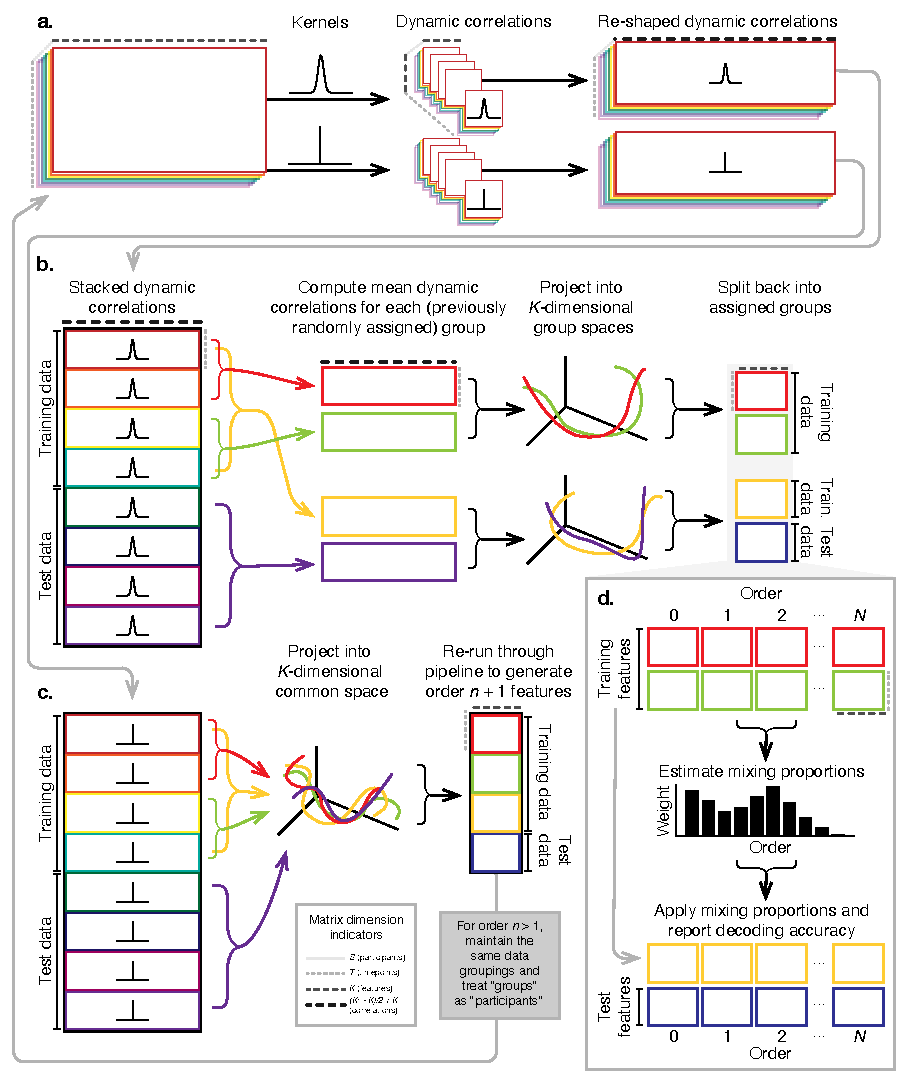
\includegraphics[width=0.85\textwidth]{figs/timecorr_pipeline}
  \caption{\textbf{Decoding analysis pipeline.  a. Computing dynamic
       correlations from timeseries data.}  Given a timeseries of
    observations as a $T \times K$ matrix (or a set of $S$ such
    matrices), we use Equation~\ref{eqn:timecorr} to compute each
    participant's DISFC (relative to other participants in the
    training or test sub-group, as appropriate). We repeat this
    process twice-- once using the analysis kernel (shown here as a
    Gaussian in the upper row of the panel), and once using a $\delta$
    function kernel (lower row of the panel).
    \textbf{b. Projecting
       dynamic correlations into a lower-dimensional space.}  We
    project the training and test data into $K$-dimensional spaces to
    create compact representations of dynamic correlations at the
    given order (estimated using the analysis kernel).
   \textbf{c.  Kernel trick.}  We project the dynamic correlations
    computed using a $\delta$ function kernel into a common
    $K$-dimensional space.  These low-dimensional embeddings are fed
    back through the analysis pipeline in order to compute features at
    the next-highest order. \textbf{d. Decoding analysis.}  We split
    the training data into two equal groups, and optimize the feature
    weights (i.e., dynamic correlations at each order) to maximize
    decoding accuracy.  We then apply the trained classifier to the
    (held-out) test data.
  \label{fig:pipeline}}

\end{figure}


One challenge to fairly evaluating high-order correlations is that if
the kernel used in Equation~\ref{eqn:timecorr} is wider than a single
timepoint, each repeated application of the equation will result in
further temporal blur.  Because our primary assessment metric is
temporal decoding accuracy, this unfairly biases against detecting
meaningful signal in higher-order correlations (relative to
lower-order correlations).  We attempted to mitigate temporal blur in
estimating each $\mathbf{X}_n$ by using a Dirac $\delta$ function
kernel (which places all of its mass over a single timepoint;
Fig.~\ref{fig:kernels}b, \ref{fig:pipeline}a) to compute each lower-order correlation
($\mathbf{X}_1, \mathbf{X}_2, ..., \mathbf{X}_{n-1}$).  We then used a
new (potentially wider, as described below) kernel to compute
$\mathbf{X}_{n}$ from $\mathbf{X}_{n-1}$.  In this way, temporal
blurring was applied only in the last step of computing
$\mathbf{X}_n$.  We note that, because each $\mathbf{X}_n$ is a
low-dimensional representation of the corresponding $\mathbf{Y}_n$,
the higher-order correlations we estimated reflect true correlations
in the data with lower-fidelity than estimates of lower-order
correlations.  Therefore, even after correcting for temporal blurring,
our approach is still biased against finding meaningful signal in
higher-order correlations.

After computing each
$\mathbf{X}_1, \mathbf{X}_2, ..., \mathbf{X}_{n-1}$ for each
participant, we divided participants into two equally sized groups
($\pm 1$ for odd numbers of participants):
$\mathcal{G}_{\mathrm{train}}$ and $\mathcal{G}_{\mathrm{test}}$.  We
then further subdivided $\mathcal{G}_{\mathrm{train}}$ into
$\mathcal{G}_{\mathrm{train}_1}$ and $\mathcal{G}_{\mathrm{train}_2}$.
We then computed $\mathbf{\Lambda}$ (temporal correlation) matrices
for each type of neural feature, using
$\mathcal{G}_{\mathrm{train}_1}$ and $\mathcal{G}_{\mathrm{train}_2}$.
This resulted in $n+1$ $\mathbf{\Lambda}$ matrices (one for the
original timeseries of neural activations, and one for each of $n$
orders of dynamic correlations).  Our objective was to find a set of
weights for each of these $\mathbf{\Lambda}$ matrices such that the
weighted average of the $n+1$ matrices yielded the highest decoding
accuracy.  We used quasi-Newton gradient ascent~\DIFdelbegin \DIFdel{\mbox{%DIFAUXCMD
\citep{NoceWrig06}}\hspace{0pt}%DIFAUXCMD
}\DIFdelend \DIFaddbegin \DIFadd{\mbox{%DIFAUXCMD
\cite{NoceWrig06}}\hspace{0pt}%DIFAUXCMD
}\DIFaddend ,
using decoding accuracy (for $\mathcal{G}_{\mathrm{train}_1}$ and
$\mathcal{G}_{\mathrm{train}_2}$) as the objective function to be
maximized, to find an optimal set of training data-derived weights,
$\phi_{0, 1, ..., n}$, where $\sum_{i=0}^n \phi_i = 1$ and where
$\phi_i \geq 0 \forall i \in \left[0, 1, ..., n\right]$.

After estimating an optimal set of weights, we computed a new set of
$n + 1$ $\mathbf{\Lambda}$ matrices correlating the DISFC patterns
from $\mathcal{G}_{\mathrm{train}}$ and $\mathcal{G}_{\mathrm{test}}$
at each timepoint.  We use the resulting decoding accuracy of
$\mathcal{G}_{\mathrm{test}}$ timepoints (using the weights in
$\phi_{0, 1, ..., n}$ to average the $\Lambda$ matrices) to estimate how informative
the set of neural features containing up to $n^\mathrm{th}$ order
correlations were.

We used a permutation-based procedure to form stable estimates of
decoding accuracy for each set of neural features.  In particular, we
computed the decoding accuracy for each of 10 random group assignments of
$\mathcal{G}_{\mathrm{train}}$ and $\mathcal{G}_{\mathrm{test}}$.  We
report the mean accuracy (along with 95\% confidence intervals) for each set
of neural features.


\subsubsection*{Identifying robust decoding results}
The temporal decoding procedure we use to estimate which neural
features support ongoing cognitive processing is governed by several
parameters. In particular, Equation~\ref{eqn:timecorr} requires
defining a kernel function, which can take on different shapes and
widths.  For a fixed set of neural features, each of these parameters
can yield different decoding accuracies.  Further, the best decoding
accuracy for a given timepoint may be reliably achieved by one set of
parameters, whereas the best decoding accuracy for another timepoint
might be reliably achieved by a different set of parameters, and the
best decoding accuracy across \DIFdelbegin \textit{\DIFdel{all}} %DIFAUXCMD
\DIFdelend \DIFaddbegin \DIFadd{all }\DIFaddend timepoints might be
reliably achieved by still another different set of parameters.
Rather than attempting to maximize decoding accuracy, we sought to
discover the trends in the data that were robust to classifier
parameters choices.  Specifically, we sought to characterize how
decoding accuracy varied (under different experimental conditions) as
a function of which neural features were considered.

To identify decoding results that were robust to specific classifier
parameter choices, we repeated our decoding analyses after
substituting into Equation~\ref{eqn:timecorr} each of a variety of
kernel shapes and widths.  We examined Gaussian
(Fig.~\ref{fig:kernels}c), Laplace (Fig.~\ref{fig:kernels}d), and
Mexican Hat (Fig.~\ref{fig:kernels}e) kernels, each with widths of 5,
10, 20, and 50 samples.  We then report the average decoding
accuracies across all of these parameter choices.  This enabled us to
(partially) factor out performance characteristics that were
parameter-dependent, within the set of parameters we examined.


\subsubsection*{Reverse inference}
The dynamic patterns we examined comprise high-dimensional correlation
patterns at each timepoint.  To help interpret the resulting patterns
in the context of other studies, we created summary maps by computing
the across-timepoint average pairwise correlations at each order of
analysis (first order, second order, etc.).  We selected the 10
strongest (absolute value) correlations at each order.  Each
correlation is between the dynamic activity patterns (or patterns of
dynamic high-order correlations) measured at two RBF nodes (see
\DIFdelbegin \textit{\DIFdel{Hierarchical Topographic Factor Analysis}}%DIFAUXCMD
\DIFdelend \DIFaddbegin \DIFadd{Hierarchical Topographic Factor Analysis}\DIFaddend ).  Therefore, the 10
strongest correlations involved up to 20 RBF nodes.  Each RBF defines
a spatial function whose activations range from 0 to 1.  We
constructed a map of RBF components that denoted the endpoints of the
10 strongest correlations (we set each RBF to have a maximum value of
1).  We then carried out a meta analysis using
Neurosynth~\DIFdelbegin \DIFdel{\mbox{%DIFAUXCMD
\citep{RubiEtal17} }\hspace{0pt}%DIFAUXCMD
}\DIFdelend \DIFaddbegin \DIFadd{\mbox{%DIFAUXCMD
\cite{RubiEtal17} }\hspace{0pt}%DIFAUXCMD
}\DIFaddend to identify the 10 terms most commonly
associated with the given map.  This resulted in a set of 10 terms
associated with the average dynamic correlation patterns at each
order.

\DIFaddbegin \section*{\DIFadd{Data Availability}}

\DIFadd{The authors declare that the data supporting the findings of this
study as well as the source data for this paper are available at
}\href{https://github.com/ContextLab/timecorr-paper/releases/tag/v0.4}{github.com/ContextLab/timecorr-paper/releases/tag/v0.4}
\DIFadd{and has been deposited in the Zenodo database under accession code
}\href{https://doi.org/10.5281/zenodo.5165253}{https://doi.org/10.5281/zenodo.5165253}\DIFadd{.
The source data underlying Figs. 2-6 and Supplementary Figs. S1-S9 are
provided as a Source Data file. Source Data are provided with the
manuscript. The raw fMRI data are protected and are not available due to data
privacy laws. The processed fMRI dataset collected by
\mbox{%DIFAUXCMD
\cite{SimoEtal16} }\hspace{0pt}%DIFAUXCMD
has been made publicly available \mbox{%DIFAUXCMD
\cite{SimoEtal16b} }\hspace{0pt}%DIFAUXCMD
at
}\href{http://arks.princeton.edu/ark:/88435/dsp015d86p269k}{arks.princeton.edu/ark:/88435/dsp015d86p269k}\DIFadd{. 
}

\section*{\DIFadd{Code Availability}}

\DIFadd{All of our analysis code may be downloaded from
}\href{https://github.com/ContextLab/timecorr-paper/releases/tag/v0.3}{github.com/ContextLab/timecorr-paper/releases/tag/v0.4}\DIFadd{. We have also published a companion Python toolbox that may be downloaded from }\href{https://timecorr.readthedocs.io}{timecorr.readthedocs.io}\DIFadd{.
}


\DIFaddend \section*{Acknowledgements}
We acknowledge discussions with Luke Chang, Vassiki Chauhan, Hany
Farid, Paxton Fitzpatrick, Andrew Heusser, Eshin Jolly, Aaron Lee,
Qiang Liu, Matthijs van der Meer, Judith Mildner, Gina Notaro, Stephen
Satterthwaite, Emily Whitaker, Weizhen Xie, and Kirsten Ziman. Our
work was supported in part by NSF EPSCoR Award Number 1632738 to
J.R.M. and by a sub-award of DARPA RAM Cooperative Agreement
N66001-14-2-4-032 to J.R.M.  The content is solely the responsibility
of the authors and does not necessarily represent the official views
of our supporting organizations.

\section*{Author contributions}
Concept: J.R.M.  Implementation: T.H.C., L.L.W.O., and J.R.M.
Analyses: L.L.W.O. and J.R.M.  Writing: L.L.W.O. and J.R.M.

\DIFdelbegin %DIFDELCMD < \bibliographystyle{apacite}
%DIFDELCMD < \bibliography{CDL-bibliography/cdl}
%DIFDELCMD < %%%
\DIFdelend \DIFaddbegin \section*{\DIFadd{Competing interests}}
\DIFadd{The authors declare no competing interests.
}

\bibliographystyle{naturemag}
%DIF > \bibliography{CDL-bibliography/cdl}

\begin{thebibliography}{10}
\expandafter\ifx\csname \DIFadd{url}\endcsname\relax
  \def\url#1{\texttt{#1}}\fi
\expandafter\ifx\csname \DIFadd{urlprefix}\endcsname\relax\def\urlprefix{URL }\fi
\providecommand{\bibinfo}[2]{#2}
\providecommand{\eprint}[2][]{\url{#2}}

\bibitem{HaxbEtal01}
\bibinfo{author}{Haxby, J.~V.} \emph{\DIFadd{et~al.}}
\newblock \bibinfo{title}{Distributed and overlapping representations of faces
  and objects in ventral temporal cortex}\DIFadd{.
}\newblock \emph{\bibinfo{journal}{Science}} \textbf{\bibinfo{volume}{293}}\DIFadd{,
  }\bibinfo{pages}{2425--2430} \DIFadd{(}\bibinfo{year}{2001}\DIFadd{).
}

\bibitem{NormEtal06b}
\bibinfo{author}{Norman, K.~A.}\DIFadd{, }\bibinfo{author}{Polyn, S.~M.}\DIFadd{,
  }\bibinfo{author}{Detre, G.~J.} \DIFadd{\& }\bibinfo{author}{Haxby, J.~V.}
\newblock \bibinfo{title}{Beyond mind-reading: multi-voxel pattern analysis of
  {fMRI} data}\DIFadd{.
}\newblock \emph{\bibinfo{journal}{Trends in Cognitive Sciences}}
  \textbf{\bibinfo{volume}{10}}\DIFadd{, }\bibinfo{pages}{424--430}
  \DIFadd{(}\bibinfo{year}{2006}\DIFadd{).
}

\bibitem{TongPrat12}
\bibinfo{author}{Tong, F.} \DIFadd{\& }\bibinfo{author}{Pratte, M.~S.}
\newblock \bibinfo{title}{Decoding patterns of human brain activity}\DIFadd{.
}\newblock \emph{\bibinfo{journal}{Annual Review of Psychology}}
  \textbf{\bibinfo{volume}{63}}\DIFadd{, }\bibinfo{pages}{483--509}
  \DIFadd{(}\bibinfo{year}{2012}\DIFadd{).
}

\bibitem{MitcEtal08a}
\bibinfo{author}{Mitchell, T.~M.} \emph{\DIFadd{et~al.}}
\newblock \bibinfo{title}{Predicting human brain activity associated with the
  meanings of nouns}\DIFadd{.
}\newblock \emph{\bibinfo{journal}{Science}} \textbf{\bibinfo{volume}{320}}\DIFadd{,
  }\bibinfo{pages}{1191} \DIFadd{(}\bibinfo{year}{2008}\DIFadd{).
}

\bibitem{KamiTong05}
\bibinfo{author}{Kamitani, Y.} \DIFadd{\& }\bibinfo{author}{Tong, F.}
\newblock \bibinfo{title}{Decoding the visual and subjective contents of the
  human brain}\DIFadd{.
}\newblock \emph{\bibinfo{journal}{Nature Neuroscience}}
  \textbf{\bibinfo{volume}{8}}\DIFadd{, }\bibinfo{pages}{679--685}
  \DIFadd{(}\bibinfo{year}{2005}\DIFadd{).
}

\bibitem{NishEtal11}
\bibinfo{author}{Nishimoto, S.} \emph{\DIFadd{et~al.}}
\newblock \bibinfo{title}{Reconstructing visual experience from brain activity
  evoked by natural movies}\DIFadd{.
}\newblock \emph{\bibinfo{journal}{Current Biology}}
  \textbf{\bibinfo{volume}{21}}\DIFadd{, }\bibinfo{pages}{1--6} \DIFadd{(}\bibinfo{year}{2011}\DIFadd{).
}

\bibitem{PereEtal18}
\bibinfo{author}{Pereira, F.} \emph{\DIFadd{et~al.}}
\newblock \bibinfo{title}{Toward a universal decoder of linguistic meaning from
  brain activation}\DIFadd{.
}\newblock \emph{\bibinfo{journal}{Nature Communications}}
  \textbf{\bibinfo{volume}{9}}\DIFadd{, }\bibinfo{pages}{1--13} \DIFadd{(}\bibinfo{year}{2018}\DIFadd{).
}

\bibitem{HuthEtal12}
\bibinfo{author}{Huth, A.~G.}\DIFadd{, }\bibinfo{author}{Nisimoto, S.}\DIFadd{,
  }\bibinfo{author}{Vu, A.~T.} \DIFadd{\& }\bibinfo{author}{Gallant, J.~L.}
\newblock \bibinfo{title}{A continuous semantic space describes the
  representation of thousands of object and action categories across the human
  brain}\DIFadd{.
}\newblock \emph{\bibinfo{journal}{Neuron}} \textbf{\bibinfo{volume}{76}}\DIFadd{,
  }\bibinfo{pages}{1210--1224} \DIFadd{(}\bibinfo{year}{2012}\DIFadd{).
}

\bibitem{HuthEtal16}
\bibinfo{author}{Huth, A.~G.}\DIFadd{, }\bibinfo{author}{de~Heer, W.~A.}\DIFadd{,
  }\bibinfo{author}{Griffiths, T.~L.}\DIFadd{, }\bibinfo{author}{Theunissen, F.~E.} \DIFadd{\&
  }\bibinfo{author}{Gallant, J.~L.}
\newblock \bibinfo{title}{Natural speech reveals the semantic maps that tile
  human cerebral cortex}\DIFadd{.
}\newblock \emph{\bibinfo{journal}{Nature}} \textbf{\bibinfo{volume}{532}}\DIFadd{,
  }\bibinfo{pages}{453--458} \DIFadd{(}\bibinfo{year}{2016}\DIFadd{).
}

\bibitem{EtzeEtal09}
\bibinfo{author}{Etzel, J.~A.}\DIFadd{, }\bibinfo{author}{Gazzola, V.} \DIFadd{\&
  }\bibinfo{author}{Keysers, C.}
\newblock \bibinfo{title}{An introduction to anatomical {ROI}-based {fMRI}
  classification}\DIFadd{.
}\newblock \emph{\bibinfo{journal}{Brain Research}}
  \textbf{\bibinfo{volume}{1281}}\DIFadd{, }\bibinfo{pages}{114--125}
  \DIFadd{(}\bibinfo{year}{2009}\DIFadd{).
}

\bibitem{MannEtal18}
\bibinfo{author}{Manning, J.~R.} \emph{\DIFadd{et~al.}}
\newblock \bibinfo{title}{A probabilistic approach to discovering dynamic
  full-brain functional connectivity patterns}\DIFadd{.
}\newblock \emph{\bibinfo{journal}{{NeuroImage}}}
  \textbf{\bibinfo{volume}{180}}\DIFadd{, }\bibinfo{pages}{243--252}
  \DIFadd{(}\bibinfo{year}{2018}\DIFadd{).
}

\bibitem{FongEtal19}
\bibinfo{author}{Fong, A. H.~C.} \emph{\DIFadd{et~al.}}
\newblock \bibinfo{title}{Dynamic functional connectivity during task
  performance and rest predicts individual differences in attention across
  studies}\DIFadd{.
}\newblock \emph{\bibinfo{journal}{{NeuroImage}}}
  \textbf{\bibinfo{volume}{188}}\DIFadd{, }\bibinfo{pages}{14--25}
  \DIFadd{(}\bibinfo{year}{2019}\DIFadd{).
}

\bibitem{Gros88}
\bibinfo{author}{Grossberg, S.}
\newblock \bibinfo{title}{Nonlinear neural networks: principles, mechanisms,
  and architectures}\DIFadd{.
}\newblock \emph{\bibinfo{journal}{Neural Networks}}
  \textbf{\bibinfo{volume}{1}}\DIFadd{, }\bibinfo{pages}{17--61} \DIFadd{(}\bibinfo{year}{1988}\DIFadd{).
}

\bibitem{Fris00}
\bibinfo{author}{Friston, K.~J.}
\newblock \bibinfo{title}{The labile brain. {I}. neuronal transients and
  nonlinear coupling}\DIFadd{.
}\newblock \emph{\bibinfo{journal}{Philosophical Transactions of the Royal
  Society of London}} \textbf{\bibinfo{volume}{355B}}\DIFadd{,
  }\bibinfo{pages}{215--236} \DIFadd{(}\bibinfo{year}{2000}\DIFadd{).
}

\bibitem{SporHone06}
\bibinfo{author}{Sporns, O.} \DIFadd{\& }\bibinfo{author}{Honey, C.~J.}
\newblock \bibinfo{title}{Small worlds inside big brains}\DIFadd{.
}\newblock \emph{\bibinfo{journal}{Proceedings of the National Academy of
  Sciences, {USA}}} \textbf{\bibinfo{volume}{103}}\DIFadd{,
  }\bibinfo{pages}{19219--19220} \DIFadd{(}\bibinfo{year}{2006}\DIFadd{).
}

\bibitem{BassEtal06}
\bibinfo{author}{Bassett, D.}\DIFadd{, }\bibinfo{author}{Meyer-Lindenberg, A.}\DIFadd{,
  }\bibinfo{author}{Achard, S.}\DIFadd{, }\bibinfo{author}{Duke, T.} \DIFadd{\&
  }\bibinfo{author}{Bullmore, E.}
\newblock \bibinfo{title}{Adaptive reconfiguration of fractal small-world human
  brain functional networks}\DIFadd{.
}\newblock \emph{\bibinfo{journal}{Proceedings of the National Academy of
  Sciences, {USA}}} \textbf{\bibinfo{volume}{103}}\DIFadd{,
  }\bibinfo{pages}{19518--19523} \DIFadd{(}\bibinfo{year}{2006}\DIFadd{).
}

\bibitem{Turk13}
\bibinfo{author}{Turk-Browne, N.~B.}
\newblock \bibinfo{title}{Functional interactions as big data in the human
  brain}\DIFadd{.
}\newblock \emph{\bibinfo{journal}{Science}} \textbf{\bibinfo{volume}{342}}\DIFadd{,
  }\bibinfo{pages}{580--584} \DIFadd{(}\bibinfo{year}{2013}\DIFadd{).
}

\bibitem{DemeEtal19}
\bibinfo{author}{Demertzi, A.} \emph{\DIFadd{et~al.}}
\newblock \bibinfo{title}{Human consciousness is supported by dynamic complex
  patterns of brain signal coordination}\DIFadd{.
}\newblock \emph{\bibinfo{journal}{Science Advances}}
  \textbf{\bibinfo{volume}{5}}\DIFadd{, }\bibinfo{pages}{eaat7603}
  \DIFadd{(}\bibinfo{year}{2019}\DIFadd{).
}

\bibitem{SoloEtal19}
\bibinfo{author}{Solomon, S.~H.}\DIFadd{, }\bibinfo{author}{Medaglia, J.~D.} \DIFadd{\&
  }\bibinfo{author}{Thompson-Schill, S.~L.}
\newblock \bibinfo{title}{Implementing a concept network model}\DIFadd{.
}\newblock \emph{\bibinfo{journal}{Behavior Research Methods}}
  \textbf{\bibinfo{volume}{51}}\DIFadd{, }\bibinfo{pages}{1717--1736}
  \DIFadd{(}\bibinfo{year}{2019}\DIFadd{).
}

\bibitem{LuriEtal18}
\bibinfo{author}{Lurie, D.} \emph{\DIFadd{et~al.}}
\newblock \bibinfo{title}{On the nature of time-varying functional connectivity
  in resting f{MRI}}\DIFadd{.
}\newblock \emph{\bibinfo{journal}{{PsyArXiv}}}
  \textbf{\bibinfo{volume}{doi.org/10.31234/osf.io/xtzre}}
  \DIFadd{(}\bibinfo{year}{2018}\DIFadd{).
}

\bibitem{PretEtal17}
\bibinfo{author}{Preti, M.~G.}\DIFadd{, }\bibinfo{author}{Bolton, T. A.~W.} \DIFadd{\&
  }\bibinfo{author}{{Van De Ville}, D.}
\newblock \bibinfo{title}{The dynamic functional connectome: state-of-the-art
  and perspectives}\DIFadd{.
}\newblock \emph{\bibinfo{journal}{{NeuroImage}}}
  \textbf{\bibinfo{volume}{160}}\DIFadd{, }\bibinfo{pages}{41--54}
  \DIFadd{(}\bibinfo{year}{2017}\DIFadd{).
}

\bibitem{ZouEtal19}
\bibinfo{author}{Zou, Y.}\DIFadd{, }\bibinfo{author}{Donner, R.~V.}\DIFadd{,
  }\bibinfo{author}{Marwan, N.}\DIFadd{, }\bibinfo{author}{Donges, J.~F.} \DIFadd{\&
  }\bibinfo{author}{Kurths, J.}
\newblock \bibinfo{title}{Complex network approaches to nonlinear time series
  analysis}\DIFadd{.
}\newblock \emph{\bibinfo{journal}{Physics Reports}}
  \textbf{\bibinfo{volume}{787}}\DIFadd{, }\bibinfo{pages}{1--97}
  \DIFadd{(}\bibinfo{year}{2019}\DIFadd{).
}

\bibitem{MackEtal17}
\bibinfo{author}{Mack, M.~L.}\DIFadd{, }\bibinfo{author}{Preston, A.~R.} \DIFadd{\&
  }\bibinfo{author}{Love, B.~C.}
\newblock \bibinfo{title}{Medial prefrontal cortex compresses concept
  representations through learning}\DIFadd{.
}\newblock \emph{\bibinfo{journal}{{bioRxiv}}}
  \textbf{\bibinfo{volume}{doi.org/10.1101/178145}} \DIFadd{(}\bibinfo{year}{2017}\DIFadd{).
}

\bibitem{BresKels01}
\bibinfo{author}{Bressler, S.~L.} \DIFadd{\& }\bibinfo{author}{Kelso, J. A.~S.}
\newblock \bibinfo{title}{Cortical coordination dynamics and cognition}\DIFadd{.
}\newblock \emph{\bibinfo{journal}{Trends in Cognitive Sciences}}
  \textbf{\bibinfo{volume}{5}}\DIFadd{, }\bibinfo{pages}{26--36} \DIFadd{(}\bibinfo{year}{2001}\DIFadd{).
}

\bibitem{McIn00}
\bibinfo{author}{McIntosh, A.~R.}
\newblock \bibinfo{title}{Towards a network theory of cognition}\DIFadd{.
}\newblock \emph{\bibinfo{journal}{Neural Networks}}
  \textbf{\bibinfo{volume}{13}}\DIFadd{, }\bibinfo{pages}{861--870}
  \DIFadd{(}\bibinfo{year}{2000}\DIFadd{).
}

\bibitem{ReimEtal17}
\bibinfo{author}{Reimann, M.~W.} \emph{\DIFadd{et~al.}}
\newblock \bibinfo{title}{Cliques of neurons bound into cavities provide a
  missing link between structure and function}\DIFadd{.
}\newblock \emph{\bibinfo{journal}{Frontiers in Computational Neuroscience}}
  \textbf{\bibinfo{volume}{11}}\DIFadd{, }\bibinfo{pages}{1--16} \DIFadd{(}\bibinfo{year}{2017}\DIFadd{).
}

\bibitem{BeatEtal16}
\bibinfo{author}{Beaty, R.~E.}\DIFadd{, }\bibinfo{author}{Benedek, M.}\DIFadd{,
  }\bibinfo{author}{Silvia, P.~J.} \DIFadd{\& }\bibinfo{author}{Schacter, D.~L.}
\newblock \bibinfo{title}{Creative cognition and brain network dynamics}\DIFadd{.
}\newblock \emph{\bibinfo{journal}{Trends in Cognitive Sciences}}
  \textbf{\bibinfo{volume}{20}}\DIFadd{, }\bibinfo{pages}{87--95}
  \DIFadd{(}\bibinfo{year}{2016}\DIFadd{).
}

\bibitem{BullSpor09}
\bibinfo{author}{Bullmore, E.} \DIFadd{\& }\bibinfo{author}{Sporns, O.}
\newblock \bibinfo{title}{Complex brain networks: graph theoretical analysis of
  structural and functional systems}\DIFadd{.
}\newblock \emph{\bibinfo{journal}{Nature Reviews Neuroscience}}
  \textbf{\bibinfo{volume}{10}}\DIFadd{, }\bibinfo{pages}{186--198}
  \DIFadd{(}\bibinfo{year}{2009}\DIFadd{).
}

\bibitem{Pear01}
\bibinfo{author}{Pearson, K.}
\newblock \bibinfo{title}{On lines and planes of closest fit to systems of
  points in space}\DIFadd{.
}\newblock \emph{\bibinfo{journal}{The London, Edinburgh, and Dublin
  Philosophical Magazine and Journal of Science}} \textbf{\bibinfo{volume}{2}}\DIFadd{,
  }\bibinfo{pages}{559--572} \DIFadd{(}\bibinfo{year}{1901}\DIFadd{).
}

\bibitem{McInJirs19}
\bibinfo{author}{Mc{I}ntosh, A.~R.} \DIFadd{\& }\bibinfo{author}{Jirsa, V.~K.}
\newblock \bibinfo{title}{The hidden repertoire of brain dynamics and
  dysfunction}\DIFadd{.
}\newblock \emph{\bibinfo{journal}{Network Neuroscience}}
  \textbf{\bibinfo{volume}{doi.org/10.1162/netn\_a\_00107}}
  \DIFadd{(}\bibinfo{year}{2019}\DIFadd{).
}

\bibitem{TokeSomm19}
\bibinfo{author}{Toker, D.} \DIFadd{\& }\bibinfo{author}{Sommer, F.~T.}
\newblock \bibinfo{title}{Information integration in large brain networks}\DIFadd{.
}\newblock \emph{\bibinfo{journal}{{PLoS} Computational Biology}}
  \textbf{\bibinfo{volume}{15}}\DIFadd{, }\bibinfo{pages}{e1006807}
  \DIFadd{(}\bibinfo{year}{2019}\DIFadd{).
}

\bibitem{GonzEtal19}
\bibinfo{author}{Gonzalez-Castillo, J.} \emph{\DIFadd{et~al.}}
\newblock \bibinfo{title}{Imaging the spontaneous flow of thought: distinct
  periods of cognition contribute to dynamic functional connectivity during
  test}\DIFadd{.
}\newblock \emph{\bibinfo{journal}{{NeuroImage}}} \textbf{\bibinfo{volume}{202}}
  \DIFadd{(}\bibinfo{year}{2019}\DIFadd{).
}

\bibitem{Land95}
\bibinfo{author}{Landau, E.}
\newblock \bibinfo{title}{Zur relativen {Wertbemessung} der
  {Turnierresultate}}\DIFadd{.
}\newblock \emph{\bibinfo{journal}{Deutsches Wochenschach}}
  \textbf{\bibinfo{volume}{11}}\DIFadd{, }\bibinfo{pages}{366--369}
  \DIFadd{(}\bibinfo{year}{1895}\DIFadd{).
}

\bibitem{BetzEtal19}
\bibinfo{author}{Betzel, R.~F.}\DIFadd{, }\bibinfo{author}{Byrge, L.}\DIFadd{,
  }\bibinfo{author}{Esfahlani, F.~Z.} \DIFadd{\& }\bibinfo{author}{Kennedy, D.~P.}
\newblock \bibinfo{title}{Temporal fluctuations in the brain's modular
  architecture during movie-watching}\DIFadd{.
}\newblock \emph{\bibinfo{journal}{{bioRxiv}}}
  \textbf{\bibinfo{volume}{doi.org/10.1101/750919}} \DIFadd{(}\bibinfo{year}{2019}\DIFadd{).
}

\bibitem{SizeEtal18}
\bibinfo{author}{Sizemore, A.~E.} \emph{\DIFadd{et~al.}}
\newblock \bibinfo{title}{Cliques and cavities in the human connectome}\DIFadd{.
}\newblock \emph{\bibinfo{journal}{Journal of Computational Neuroscience}}
  \textbf{\bibinfo{volume}{44}}\DIFadd{, }\bibinfo{pages}{115--145}
  \DIFadd{(}\bibinfo{year}{2018}\DIFadd{).
}

\bibitem{SimoEtal16}
\bibinfo{author}{Simony, E.}\DIFadd{, }\bibinfo{author}{Honey, C.~J.}\DIFadd{,
  }\bibinfo{author}{Chen, J.} \DIFadd{\& }\bibinfo{author}{Hasson, U.}
\newblock \bibinfo{title}{Dynamic reconfiguration of the default mode network
  during narrative comprehension}\DIFadd{.
}\newblock \emph{\bibinfo{journal}{Nature Communications}}
  \textbf{\bibinfo{volume}{7}}\DIFadd{, }\bibinfo{pages}{1--13} \DIFadd{(}\bibinfo{year}{2016}\DIFadd{).
}

\bibitem{HassEtal08}
\bibinfo{author}{Hasson, U.}\DIFadd{, }\bibinfo{author}{Yang, E.}\DIFadd{,
  }\bibinfo{author}{Vallines, I.}\DIFadd{, }\bibinfo{author}{Heeger, D.~J.} \DIFadd{\&
  }\bibinfo{author}{Rubin, N.}
\newblock \bibinfo{title}{A hierarchy of temporal receptive windows in human
  cortex}\DIFadd{.
}\newblock \emph{\bibinfo{journal}{The Journal of Neuroscience}}
  \textbf{\bibinfo{volume}{28}}\DIFadd{, }\bibinfo{pages}{2539--2550}
  \DIFadd{(}\bibinfo{year}{2008}\DIFadd{).
}

\bibitem{RubiEtal17}
\bibinfo{author}{Rubin, T.~N.} \emph{\DIFadd{et~al.}}
\newblock \bibinfo{title}{Decoding brain activity using a large-scale
  probabilistic functional-anatomical atlas of human cognition}\DIFadd{.
}\newblock \emph{\bibinfo{journal}{{PLoS} Computational Biology}}
  \textbf{\bibinfo{volume}{13}}\DIFadd{, }\bibinfo{pages}{e1005649}
  \DIFadd{(}\bibinfo{year}{2017}\DIFadd{).
}

\bibitem{ParkEtal18b}
\bibinfo{author}{Park, H.-J.}\DIFadd{, }\bibinfo{author}{Friston, K.~J.}\DIFadd{,
  }\bibinfo{author}{Pae, C.}\DIFadd{, }\bibinfo{author}{Park, B.} \DIFadd{\&
  }\bibinfo{author}{Razi, A.}
\newblock \bibinfo{title}{Dynamic effective connectivity in resting state
  {fMRI}}\DIFadd{.
}\newblock \emph{\bibinfo{journal}{{NeuroImage}}}
  \textbf{\bibinfo{volume}{180}}\DIFadd{, }\bibinfo{pages}{594--608}
  \DIFadd{(}\bibinfo{year}{2018}\DIFadd{).
}

\bibitem{RoyEtal19}
\bibinfo{author}{Roy, D.~S.} \emph{\DIFadd{et~al.}}
\newblock \bibinfo{title}{Brain-wide mapping of contextual fear memory engram
  ensembles supports the dispersed engram complex hypothesis}\DIFadd{.
}\newblock \emph{\bibinfo{journal}{{bioRxiv}}}
  \textbf{\bibinfo{volume}{doi.org/10.1101/668483}} \DIFadd{(}\bibinfo{year}{2019}\DIFadd{).
}

\bibitem{LiegEtal19}
\bibinfo{author}{Li\'{e}geois, R.} \emph{\DIFadd{et~al.}}
\newblock \bibinfo{title}{Resting brain dynamics at different timescales
  capture distinct aspects of human behavior}\DIFadd{.
}\newblock \emph{\bibinfo{journal}{Nature Communications}}
  \textbf{\bibinfo{volume}{10}}\DIFadd{, }\bibinfo{pages}{1--9} \DIFadd{(}\bibinfo{year}{2019}\DIFadd{).
}

\bibitem{ChanGlov10}
\bibinfo{author}{Chang, C.} \DIFadd{\& }\bibinfo{author}{Glover, G.~H.}
\newblock \bibinfo{title}{Time-frequency dynamics of resting-state brain
  connectivity measured with f{MRI}}\DIFadd{.
}\newblock \emph{\bibinfo{journal}{{NeuroImage}}} \textbf{\bibinfo{volume}{50}}\DIFadd{,
  }\bibinfo{pages}{81--98} \DIFadd{(}\bibinfo{year}{2010}\DIFadd{).
}

\bibitem{ZhenEtal19}
\bibinfo{author}{Zheng, M.}\DIFadd{, }\bibinfo{author}{Allard, A.}\DIFadd{,
  }\bibinfo{author}{Hagmann, P.} \DIFadd{\& }\bibinfo{author}{Serrano, M. . .~A.}
\newblock \bibinfo{title}{Geometric renormalization unravels self-similarity of
  the multiscale human connectome}\DIFadd{.
}\newblock \emph{\bibinfo{journal}{{arXiv}}}
  \textbf{\bibinfo{volume}{1904.11793}} \DIFadd{(}\bibinfo{year}{2019}\DIFadd{).
}

\bibitem{BaldEtal17}
\bibinfo{author}{Baldassano, C.} \emph{\DIFadd{et~al.}}
\newblock \bibinfo{title}{Discovering event structure in continuous narrative
  perception and memory}\DIFadd{.
}\newblock \emph{\bibinfo{journal}{Neuron}} \textbf{\bibinfo{volume}{95}}\DIFadd{,
  }\bibinfo{pages}{709--721} \DIFadd{(}\bibinfo{year}{2017}\DIFadd{).
}

\bibitem{HassEtal15}
\bibinfo{author}{Hasson, U.}\DIFadd{, }\bibinfo{author}{Chen, J.} \DIFadd{\&
  }\bibinfo{author}{Honey, C.~J.}
\newblock \bibinfo{title}{Hierarchical process memory: memory as an integral
  component of information processing}\DIFadd{.
}\newblock \emph{\bibinfo{journal}{Trends in Cognitive Sciences}}
  \textbf{\bibinfo{volume}{19}}\DIFadd{, }\bibinfo{pages}{304--315}
  \DIFadd{(}\bibinfo{year}{2015}\DIFadd{).
}

\bibitem{HoneEtal12a}
\bibinfo{author}{Honey, C.~J.} \emph{\DIFadd{et~al.}}
\newblock \bibinfo{title}{Slow cortical dynamics and the accumulation of
  information over long timescales}\DIFadd{.
}\newblock \emph{\bibinfo{journal}{Neuron}} \textbf{\bibinfo{volume}{76}}\DIFadd{,
  }\bibinfo{pages}{423--434} \DIFadd{(}\bibinfo{year}{2012}\DIFadd{).
}

\bibitem{LernEtal11}
\bibinfo{author}{Lerner, Y.}\DIFadd{, }\bibinfo{author}{Honey, C.~J.}\DIFadd{,
  }\bibinfo{author}{Silbert, L.~J.} \DIFadd{\& }\bibinfo{author}{Hasson, U.}
\newblock \bibinfo{title}{Topographic mapping of a hierarchy of temporal
  receptive windows using a narrated story}\DIFadd{.
}\newblock \emph{\bibinfo{journal}{The Journal of Neuroscience}}
  \textbf{\bibinfo{volume}{31}}\DIFadd{, }\bibinfo{pages}{2906--2915}
  \DIFadd{(}\bibinfo{year}{2011}\DIFadd{).
}

\bibitem{LernEtal14}
\bibinfo{author}{Lerner, Y.}\DIFadd{, }\bibinfo{author}{Honey, C.~J.}\DIFadd{,
  }\bibinfo{author}{Katkov, M.} \DIFadd{\& }\bibinfo{author}{Hasson, U.}
\newblock \bibinfo{title}{Temporal scaling of neural responses to compressed
  and dilated natural speech}\DIFadd{.
}\newblock \emph{\bibinfo{journal}{Journal of Neurophysiology}}
  \textbf{\bibinfo{volume}{111}}\DIFadd{, }\bibinfo{pages}{2433--2444}
  \DIFadd{(}\bibinfo{year}{2014}\DIFadd{).
}

\bibitem{ChieHone19}
\bibinfo{author}{Chien, H.-Y.~S.} \DIFadd{\& }\bibinfo{author}{Honey, C.~J.}
\newblock \bibinfo{title}{Constructing and forgetting temporal context in the
  human cerebral cortex}\DIFadd{.
}\newblock \emph{\bibinfo{journal}{{bioRxiv}}}
  \textbf{\bibinfo{volume}{doi.org/10.1101/761593}} \DIFadd{(}\bibinfo{year}{2019}\DIFadd{).
}

\bibitem{LeeEtal20}
\bibinfo{author}{Lee, C.~S.}\DIFadd{, }\bibinfo{author}{Aly, M.} \DIFadd{\&
  }\bibinfo{author}{Baldassano, C.}
\newblock \bibinfo{title}{Anticipation of temporally structured events in the
  brain}\DIFadd{.
}\newblock \emph{\bibinfo{journal}{{bioRxiv}}}
  \textbf{\bibinfo{volume}{10.1101/2020.10.14.338145}} \DIFadd{(}\bibinfo{year}{2020}\DIFadd{).
}

\bibitem{FallEtal20}
\bibinfo{author}{Fallon, J.}\DIFadd{, }\bibinfo{author}{Ward, P. G.~D.}\DIFadd{,
  }\bibinfo{author}{Parkes, L.} \DIFadd{\& }\bibinfo{author}{Oldham, S.}
\newblock \bibinfo{title}{Timescales of spontaneous {fMRI} fluctuations relate
  to structural connectivity in the brain}\DIFadd{.
}\newblock \emph{\bibinfo{journal}{Network Neuroscience}}
  \textbf{\bibinfo{volume}{4}}\DIFadd{, }\bibinfo{pages}{788--806}
  \DIFadd{(}\bibinfo{year}{2020}\DIFadd{).
}

\bibitem{ShapEtal19}
\bibinfo{author}{Shappell, H.}\DIFadd{, }\bibinfo{author}{Caffo, B.~S.}\DIFadd{,
  }\bibinfo{author}{Pekar, J.~J.} \DIFadd{\& }\bibinfo{author}{Lindquist, M.~A.}
\newblock \bibinfo{title}{Improved state change estimation in dynamic
  functional connectivity using hidden semi-{M}arkov models}\DIFadd{.
}\newblock \emph{\bibinfo{journal}{{NeuroImage}}}
  \textbf{\bibinfo{volume}{191}}\DIFadd{, }\bibinfo{pages}{243--257}
  \DIFadd{(}\bibinfo{year}{2019}\DIFadd{).
}

\bibitem{VidaEtal18}
\bibinfo{author}{Vidaurre, D.} \emph{\DIFadd{et~al.}}
\newblock \bibinfo{title}{Discovering dynamic brain neworks from big data in
  rest and task}\DIFadd{.
}\newblock \emph{\bibinfo{journal}{{NeuroImage}}}
  \textbf{\bibinfo{volume}{180}}\DIFadd{, }\bibinfo{pages}{646--656}
  \DIFadd{(}\bibinfo{year}{2018}\DIFadd{).
}

\bibitem{AlleEtal12b}
\bibinfo{author}{Allen, E.~A.} \emph{\DIFadd{et~al.}}
\newblock \bibinfo{title}{Tracking whole-brain connectivity dynamics in the
  resting state}\DIFadd{.
}\newblock \emph{\bibinfo{journal}{Cerebral Cortex}}
  \textbf{\bibinfo{volume}{24}}\DIFadd{, }\bibinfo{pages}{663--676}
  \DIFadd{(}\bibinfo{year}{2012}\DIFadd{).
}

\bibitem{SimoChan20}
\bibinfo{author}{Simony, E.} \DIFadd{\& }\bibinfo{author}{Chang, C.}
\newblock \bibinfo{title}{Analysis of stimulus-induced brain dynamics during
  naturalistic paradigms}\DIFadd{.
}\newblock \emph{\bibinfo{journal}{{NeuroImage}}}
  \textbf{\bibinfo{volume}{216}}\DIFadd{, }\bibinfo{pages}{116461}
  \DIFadd{(}\bibinfo{year}{2020}\DIFadd{).
}

\bibitem{Zar10}
\bibinfo{author}{Zar, J.~H.}
\newblock \emph{\bibinfo{title}{Biostatistical analysis}}
  \DIFadd{(}\bibinfo{publisher}{Prentice-Hall}\DIFadd{, }\bibinfo{year}{2010}\DIFadd{).
}

\bibitem{TippBish99}
\bibinfo{author}{Tipping, M.~E.} \DIFadd{\& }\bibinfo{author}{Bishop, C.~M.}
\newblock \bibinfo{title}{Probabilistic principal component analysis}\DIFadd{.
}\newblock \emph{\bibinfo{journal}{Journal of Royal Statistical Society, Series
  {B}}} \textbf{\bibinfo{volume}{61}}\DIFadd{, }\bibinfo{pages}{611--622}
  \DIFadd{(}\bibinfo{year}{1999}\DIFadd{).
}

\bibitem{Spea04}
\bibinfo{author}{Spearman, C.}
\newblock \bibinfo{title}{General intelligence, objectively determined and
  measured}\DIFadd{.
}\newblock \emph{\bibinfo{journal}{Americal Journal of Psychology}}
  \textbf{\bibinfo{volume}{15}}\DIFadd{, }\bibinfo{pages}{201--292}
  \DIFadd{(}\bibinfo{year}{1904}\DIFadd{).
}

\bibitem{JuttHera91}
\bibinfo{author}{Jutten, C.} \DIFadd{\& }\bibinfo{author}{Herault, J.}
\newblock \bibinfo{title}{Blind separation of sources, part {I}: an adaptive
  algorithm based on neuromimetic architecture}\DIFadd{.
}\newblock \emph{\bibinfo{journal}{Signal Processing}}
  \textbf{\bibinfo{volume}{24}}\DIFadd{, }\bibinfo{pages}{1--10} \DIFadd{(}\bibinfo{year}{1991}\DIFadd{).
}

\bibitem{ComoEtal91}
\bibinfo{author}{Comon, P.}\DIFadd{, }\bibinfo{author}{Jutten, C.} \DIFadd{\&
  }\bibinfo{author}{Herault, J.}
\newblock \bibinfo{title}{Blind separation of sources, part {II}: problems
  statement}\DIFadd{.
}\newblock \emph{\bibinfo{journal}{Signal Processing}}
  \textbf{\bibinfo{volume}{24}}\DIFadd{, }\bibinfo{pages}{11--20}
  \DIFadd{(}\bibinfo{year}{1991}\DIFadd{).
}

\bibitem{vandHint08}
\bibinfo{author}{van~der Maaten, L. J.~P.} \DIFadd{\& }\bibinfo{author}{Hinton, G.~E.}
\newblock \bibinfo{title}{Visualizing high-dimensional data using {t-SNE}}\DIFadd{.
}\newblock \emph{\bibinfo{journal}{Journal of Machine Learning Research}}
  \textbf{\bibinfo{volume}{9}}\DIFadd{, }\bibinfo{pages}{2579--2605}
  \DIFadd{(}\bibinfo{year}{2008}\DIFadd{).
}

\bibitem{McInEtal18}
\bibinfo{author}{McInnes, L.}\DIFadd{, }\bibinfo{author}{Healy, J.} \DIFadd{\&
  }\bibinfo{author}{Melville, J.}
\newblock \bibinfo{title}{{UMAP}: uniform manifold approximation and projection
  for dimension reduction}\DIFadd{.
}\newblock \emph{\bibinfo{journal}{{arXiv}}} \textbf{\bibinfo{volume}{1802}}
  \DIFadd{(}\bibinfo{year}{2018}\DIFadd{).
}

\bibitem{LeeSeun99}
\bibinfo{author}{Lee, D.~D.} \DIFadd{\& }\bibinfo{author}{Seung, H.~S.}
\newblock \bibinfo{title}{Learning the parts of objects by non-negative matrix
  factorization}\DIFadd{.
}\newblock \emph{\bibinfo{journal}{Nature}} \textbf{\bibinfo{volume}{401}}\DIFadd{,
  }\bibinfo{pages}{788--791} \DIFadd{(}\bibinfo{year}{1999}\DIFadd{).
}

\bibitem{MannEtal14b}
\bibinfo{author}{Manning, J.~R.}\DIFadd{, }\bibinfo{author}{Ranganath, R.}\DIFadd{,
  }\bibinfo{author}{Norman, K.~A.} \DIFadd{\& }\bibinfo{author}{Blei, D.~M.}
\newblock \bibinfo{title}{Topographic factor analysis: a {B}ayesian model for
  inferring brain networks from neural data}\DIFadd{.
}\newblock \emph{\bibinfo{journal}{{PLoS} One}} \textbf{\bibinfo{volume}{9}}\DIFadd{,
  }\bibinfo{pages}{e94914} \DIFadd{(}\bibinfo{year}{2014}\DIFadd{).
}

\bibitem{GersEtal11}
\bibinfo{author}{Gershman, S.~J.}\DIFadd{, }\bibinfo{author}{Blei, D.~M.}\DIFadd{,
  }\bibinfo{author}{Pereira, F.} \DIFadd{\& }\bibinfo{author}{Norman, K.~A.}
\newblock \bibinfo{title}{A topographic latent source model for {fMRI} data}\DIFadd{.
}\newblock \emph{\bibinfo{journal}{{NeuroImage}}} \textbf{\bibinfo{volume}{57}}\DIFadd{,
  }\bibinfo{pages}{89--100} \DIFadd{(}\bibinfo{year}{2011}\DIFadd{).
}

\bibitem{MairEtal09a}
\bibinfo{author}{Mairal, J.~B.}\DIFadd{, }\bibinfo{author}{Bach, F.}\DIFadd{,
  }\bibinfo{author}{Ponce, J.} \DIFadd{\& }\bibinfo{author}{Sapiro, G.}
\newblock \bibinfo{title}{Online dictionary learning for sparse coding}\DIFadd{.
}\newblock \emph{\bibinfo{journal}{Proceedings of the International Conference
  on Machine Learning}} \bibinfo{pages}{689--696} \DIFadd{(}\bibinfo{year}{2009}\DIFadd{).
}

\bibitem{MairEtal09b}
\bibinfo{author}{Mairal, J.}\DIFadd{, }\bibinfo{author}{Ponce, J.}\DIFadd{,
  }\bibinfo{author}{Sapiro, G.}\DIFadd{, }\bibinfo{author}{Zisserman, A.} \DIFadd{\&
  }\bibinfo{author}{Bach, F.~R.}
\newblock \bibinfo{title}{Supervised dictionary learning}\DIFadd{.
}\newblock \emph{\bibinfo{journal}{Advances in Neural Information Processing
  Systems}} \bibinfo{pages}{1033--1040} \DIFadd{(}\bibinfo{year}{2009}\DIFadd{).
}

\bibitem{HintSala06}
\bibinfo{author}{Hinton, G.~E.} \DIFadd{\& }\bibinfo{author}{Salakhutdinov, R.~R.}
\newblock \bibinfo{title}{Reducing the dimensionality of data with neural
  networks}\DIFadd{.
}\newblock \emph{\bibinfo{journal}{Science}} \textbf{\bibinfo{volume}{313}}\DIFadd{,
  }\bibinfo{pages}{504--507} \DIFadd{(}\bibinfo{year}{2006}\DIFadd{).
}

\bibitem{Newm05}
\bibinfo{author}{Newman, M. E.~J.}
\newblock \bibinfo{title}{A measure of betweenness centrality based on random
  walks}\DIFadd{.
}\newblock \emph{\bibinfo{journal}{Social Networks}}
  \textbf{\bibinfo{volume}{27}}\DIFadd{, }\bibinfo{pages}{39--54}
  \DIFadd{(}\bibinfo{year}{2005}\DIFadd{).
}

\bibitem{OpsaEtal10}
\bibinfo{author}{Opsahl, T.}\DIFadd{, }\bibinfo{author}{Agneessens, F.} \DIFadd{\&
  }\bibinfo{author}{Skvoretz, J.}
\newblock \bibinfo{title}{Node centrality in weighted networks: generalizing
  degree and shortest paths}\DIFadd{.
}\newblock \emph{\bibinfo{journal}{Social Networks}}
  \textbf{\bibinfo{volume}{32}}\DIFadd{, }\bibinfo{pages}{245--251}
  \DIFadd{(}\bibinfo{year}{2010}\DIFadd{).
}

\bibitem{Bart04}
\bibinfo{author}{Barth\'{e}lemy, M.}
\newblock \bibinfo{title}{Betweenness centrality in large complex networks}\DIFadd{.
}\newblock \emph{\bibinfo{journal}{{European} Physical Journal {B}}}
  \textbf{\bibinfo{volume}{38}}\DIFadd{, }\bibinfo{pages}{163--168}
  \DIFadd{(}\bibinfo{year}{2004}\DIFadd{).
}

\bibitem{GeisEtal08}
\bibinfo{author}{Geisberger, R.}\DIFadd{, }\bibinfo{author}{Sanders, P.} \DIFadd{\&
  }\bibinfo{author}{Schultes, D.}
\newblock \bibinfo{title}{Better approximation of betweenness centrality}\DIFadd{.
}\newblock \emph{\bibinfo{journal}{Proceedings of the Meeting on Algorithm
  Engineering and Experiments}} \bibinfo{pages}{90--100}
  \DIFadd{(}\bibinfo{year}{2008}\DIFadd{).
}

\bibitem{Free77}
\bibinfo{author}{Freeman, L.~C.}
\newblock \bibinfo{title}{A set of measures of centrality based on
  betweenness}\DIFadd{.
}\newblock \emph{\bibinfo{journal}{Sociometry}} \textbf{\bibinfo{volume}{40}}\DIFadd{,
  }\bibinfo{pages}{35--41} \DIFadd{(}\bibinfo{year}{1977}\DIFadd{).
}

\bibitem{Rao82}
\bibinfo{author}{Rao, C.~R.}
\newblock \bibinfo{title}{Diversity and dissimilarity coeficients: a unified
  approach}\DIFadd{.
}\newblock \emph{\bibinfo{journal}{Theoretical Population Biology}}
  \textbf{\bibinfo{volume}{21}}\DIFadd{, }\bibinfo{pages}{24--43}
  \DIFadd{(}\bibinfo{year}{1982}\DIFadd{).
}

\bibitem{Lin09}
\bibinfo{author}{Lin, J.}
\newblock \bibinfo{title}{Divergence measures based on the {Shannon} entropy}\DIFadd{.
}\newblock \emph{\bibinfo{journal}{{IEEE} Transactions on Information Theory}}
  \textbf{\bibinfo{volume}{37}}\DIFadd{, }\bibinfo{pages}{145--151}
  \DIFadd{(}\bibinfo{year}{2009}\DIFadd{).
}

\bibitem{RicoSzei06}
\bibinfo{author}{Ricotta, C.} \DIFadd{\& }\bibinfo{author}{Szeidl, L.}
\newblock \bibinfo{title}{Towards a unifying approach to diversity measures:
  bridging the gap between the {Shannon} entropy and {Rao's} quadratic index}\DIFadd{.
}\newblock \emph{\bibinfo{journal}{Theoretical Population Biology}}
  \textbf{\bibinfo{volume}{70}}\DIFadd{, }\bibinfo{pages}{237--243}
  \DIFadd{(}\bibinfo{year}{2006}\DIFadd{).
}

\bibitem{Newm08}
\bibinfo{author}{Newman, M. E.~J.}
\newblock \bibinfo{title}{The mathematics of networks}\DIFadd{.
}\newblock \emph{\bibinfo{journal}{The New Palgrave Encyclopedia of Economics}}
  \textbf{\bibinfo{volume}{2}}\DIFadd{, }\bibinfo{pages}{1--12} \DIFadd{(}\bibinfo{year}{2008}\DIFadd{).
}

\bibitem{Bona07}
\bibinfo{author}{Bonacich, P.}
\newblock \bibinfo{title}{Some unique properties of eigenvector centrality}\DIFadd{.
}\newblock \emph{\bibinfo{journal}{Social Networks}}
  \textbf{\bibinfo{volume}{29}}\DIFadd{, }\bibinfo{pages}{555--564}
  \DIFadd{(}\bibinfo{year}{2007}\DIFadd{).
}

\bibitem{LohmEtal10}
\bibinfo{author}{Lohmann, G.} \emph{\DIFadd{et~al.}}
\newblock \bibinfo{title}{Eigenvector centrality mapping for analyzing
  connectivity patterns in {fMRI} data of the human brain}\DIFadd{.
}\newblock \emph{\bibinfo{journal}{{PLoS} One}} \textbf{\bibinfo{volume}{5}}\DIFadd{,
  }\bibinfo{pages}{e10232} \DIFadd{(}\bibinfo{year}{2010}\DIFadd{).
}

\bibitem{HaluEtal13}
\bibinfo{author}{Halu, A.}\DIFadd{, }\bibinfo{author}{Mondrag\'{o}n, R.~J.}\DIFadd{,
  }\bibinfo{author}{Panzarasa, P.} \DIFadd{\& }\bibinfo{author}{Bianconi, G.}
\newblock \bibinfo{title}{Multiplex {PageRank}}\DIFadd{.
}\newblock \emph{\bibinfo{journal}{{PLoS} One}} \textbf{\bibinfo{volume}{8}}\DIFadd{,
  }\bibinfo{pages}{e78293} \DIFadd{(}\bibinfo{year}{2013}\DIFadd{).
}

\bibitem{HoneEtal07}
\bibinfo{author}{Honey, C.~J.}\DIFadd{, }\bibinfo{author}{K\"{o}tter, R.}\DIFadd{,
  }\bibinfo{author}{Breakspear, M.} \DIFadd{\& }\bibinfo{author}{Sporns, O.}
\newblock \bibinfo{title}{Network structure of cerebral cortex shapes
  functional connectivity on multiple time scales}\DIFadd{.
}\newblock \emph{\bibinfo{journal}{Proceedings of the National Academy of
  Sciences, {USA}}} \textbf{\bibinfo{volume}{104}}\DIFadd{,
  }\bibinfo{pages}{10240--10245} \DIFadd{(}\bibinfo{year}{2007}\DIFadd{).
}

\bibitem{Schr00}
\bibinfo{author}{Schreiber, T.}
\newblock \bibinfo{title}{Measuring information transfer}\DIFadd{.
}\newblock \emph{\bibinfo{journal}{Physical Review Letters}}
  \textbf{\bibinfo{volume}{85}}\DIFadd{, }\bibinfo{pages}{461--464}
  \DIFadd{(}\bibinfo{year}{2000}\DIFadd{).
}

\bibitem{AlvaEtal05}
\bibinfo{author}{Alvarez-Hamelin, I.}\DIFadd{, }\bibinfo{author}{Dall'Asta, L.}\DIFadd{,
  }\bibinfo{author}{Barrat, A.} \DIFadd{\& }\bibinfo{author}{Vespignani, A.}
\newblock \bibinfo{title}{$k$-corr decomposition: a tool for the visualiztion
  of large scale networks}\DIFadd{.
}\newblock \emph{\bibinfo{journal}{{arXiv}}} \bibinfo{pages}{cs/0504107v2}
  \DIFadd{(}\bibinfo{year}{2005}\DIFadd{).
}

\bibitem{ChriFowl10}
\bibinfo{author}{Christakis, N.~A.} \DIFadd{\& }\bibinfo{author}{Fowler, J.~H.}
\newblock \bibinfo{title}{Social network sensors for early detection of
  contagious outbreaks}\DIFadd{.
}\newblock \emph{\bibinfo{journal}{{PLoS} One}} \textbf{\bibinfo{volume}{5}}\DIFadd{,
  }\bibinfo{pages}{e12948} \DIFadd{(}\bibinfo{year}{2010}\DIFadd{).
}

\bibitem{RubiSpor10}
\bibinfo{author}{Rubinov, M.} \DIFadd{\& }\bibinfo{author}{Sporns, O.}
\newblock \bibinfo{title}{Complex network measures of brain connectivity: uses
  and interpretations}\DIFadd{.
}\newblock \emph{\bibinfo{journal}{{NeuroImage}}} \textbf{\bibinfo{volume}{52}}\DIFadd{,
  }\bibinfo{pages}{1059--1069} \DIFadd{(}\bibinfo{year}{2010}\DIFadd{).
}

\bibitem{EstrRodr05}
\bibinfo{author}{Estrada, E.} \DIFadd{\& }\bibinfo{author}{Rodr\'{i}guez-Vel\'{a}zquez,
  J.~A.}
\newblock \bibinfo{title}{Subraph centrality in complex networks}\DIFadd{.
}\newblock \emph{\bibinfo{journal}{Physical Review {E}}}
  \textbf{\bibinfo{volume}{71}}\DIFadd{, }\bibinfo{pages}{056103}
  \DIFadd{(}\bibinfo{year}{2005}\DIFadd{).
}

\bibitem{ThomEtal18}
\bibinfo{author}{Thompson, W.~H.}\DIFadd{, }\bibinfo{author}{Richter, C.~G.}\DIFadd{,
  }\bibinfo{author}{Plav\'{e}n-Sigray, P.} \DIFadd{\& }\bibinfo{author}{Fransson, P.}
\newblock \bibinfo{title}{Simulations to benchmark time-varying connectivity
  methods for f{MRI}}\DIFadd{.
}\newblock \emph{\bibinfo{journal}{{PLoS} Computational Biology}}
  \textbf{\bibinfo{volume}{14}}\DIFadd{, }\bibinfo{pages}{e1006196}
  \DIFadd{(}\bibinfo{year}{2018}\DIFadd{).
}

\bibitem{CapoEtal17}
\bibinfo{author}{Capota, M.} \emph{\DIFadd{et~al.}}
\newblock \bibinfo{title}{Brain imaging analysis kit} \DIFadd{(}\bibinfo{year}{2017}\DIFadd{).
}

\bibitem{NoceWrig06}
\bibinfo{author}{Nocedal, J.} \DIFadd{\& }\bibinfo{author}{Wright, S.~J.}
\newblock \emph{\bibinfo{title}{Numerical optimization}}
  \DIFadd{(}\bibinfo{publisher}{Springer}\DIFadd{, }\bibinfo{address}{New York, {NY}}\DIFadd{,
  }\bibinfo{year}{2006}\DIFadd{).
}

\bibitem{CombEtal19}
\bibinfo{author}{Combrisson, E.} \emph{\DIFadd{et~al.}}
\newblock \bibinfo{title}{Visbrain: a multi-purpose {GPU}-accelerated
  open-source suite for multimodal brain data visualization}\DIFadd{.
}\newblock \emph{\bibinfo{journal}{Frontiers in Neuroinformatics}}
  \textbf{\bibinfo{volume}{13}}\DIFadd{, }\bibinfo{pages}{1--14}
  \DIFadd{(}\bibinfo{year}{2019}\DIFadd{).
}

\bibitem{SimoEtal16b}
\bibinfo{author}{Simony, E.}\DIFadd{, }\bibinfo{author}{Honey, C.~J.}\DIFadd{,
  }\bibinfo{author}{Chen, J.} \DIFadd{\& }\bibinfo{author}{Hasson, U.}
\newblock \bibinfo{title}{Dynamic reconfiguration of the default mode network
  during narrative comprehension}\DIFadd{.
}\newblock \emph{\bibinfo{journal}{DataSpace}}
  \textbf{\bibinfo{volume}{http://arks.princeton.edu/ark:/88435/dsp015d86p269k}} \DIFadd{(}\bibinfo{year}{2016}\DIFadd{). 
}

\end{thebibliography}
\DIFaddend 


\end{document}


